% Options for packages loaded elsewhere
\PassOptionsToPackage{unicode}{hyperref}
\PassOptionsToPackage{hyphens}{url}
%
\documentclass[
]{article}
\usepackage{lmodern}
\usepackage{setspace}
\usepackage{amsmath}
\usepackage{ifxetex,ifluatex}
\ifnum 0\ifxetex 1\fi\ifluatex 1\fi=0 % if pdftex
  \usepackage[T1]{fontenc}
  \usepackage[utf8]{inputenc}
  \usepackage{textcomp} % provide euro and other symbols
  \usepackage{amssymb}
\else % if luatex or xetex
  \usepackage{unicode-math}
  \defaultfontfeatures{Scale=MatchLowercase}
  \defaultfontfeatures[\rmfamily]{Ligatures=TeX,Scale=1}
\fi
% Use upquote if available, for straight quotes in verbatim environments
\IfFileExists{upquote.sty}{\usepackage{upquote}}{}
\IfFileExists{microtype.sty}{% use microtype if available
  \usepackage[]{microtype}
  \UseMicrotypeSet[protrusion]{basicmath} % disable protrusion for tt fonts
}{}
\usepackage{xcolor}
\IfFileExists{xurl.sty}{\usepackage{xurl}}{} % add URL line breaks if available
\IfFileExists{bookmark.sty}{\usepackage{bookmark}}{\usepackage{hyperref}}
\hypersetup{
  pdftitle={Manuscript: Detecting differences in Size Spectra},
  pdfauthor={Justin Pomeranz1,; James R. Junker2,3; Vojsava Gjoni4; Jeff S. Wesner4},
  hidelinks,
  pdfcreator={LaTeX via pandoc}}
\urlstyle{same} % disable monospaced font for URLs
\usepackage[margin=1in]{geometry}
\usepackage{longtable,booktabs}
\usepackage{calc} % for calculating minipage widths
% Correct order of tables after \paragraph or \subparagraph
\usepackage{etoolbox}
\makeatletter
\patchcmd\longtable{\par}{\if@noskipsec\mbox{}\fi\par}{}{}
\makeatother
% Allow footnotes in longtable head/foot
\IfFileExists{footnotehyper.sty}{\usepackage{footnotehyper}}{\usepackage{footnote}}
\makesavenoteenv{longtable}
\usepackage{graphicx}
\makeatletter
\def\maxwidth{\ifdim\Gin@nat@width>\linewidth\linewidth\else\Gin@nat@width\fi}
\def\maxheight{\ifdim\Gin@nat@height>\textheight\textheight\else\Gin@nat@height\fi}
\makeatother
% Scale images if necessary, so that they will not overflow the page
% margins by default, and it is still possible to overwrite the defaults
% using explicit options in \includegraphics[width, height, ...]{}
\setkeys{Gin}{width=\maxwidth,height=\maxheight,keepaspectratio}
% Set default figure placement to htbp
\makeatletter
\def\fps@figure{htbp}
\makeatother
\setlength{\emergencystretch}{3em} % prevent overfull lines
\providecommand{\tightlist}{%
  \setlength{\itemsep}{0pt}\setlength{\parskip}{0pt}}
\setcounter{secnumdepth}{-\maxdimen} % remove section numbering
\usepackage{lineno}
\usepackage{amsmath}
\usepackage{indentfirst}
\linenumbers
\newcommand{\beginsupplement}{ \setcounter{table}{0} \renewcommand{\thetable}{S\arabic{table}} \setcounter{figure}{0} \renewcommand{\thefigure}{S\arabic{figure}}}
\ifluatex
  \usepackage{selnolig}  % disable illegal ligatures
\fi
\newlength{\cslhangindent}
\setlength{\cslhangindent}{1.5em}
\newlength{\csllabelwidth}
\setlength{\csllabelwidth}{3em}
\newenvironment{CSLReferences}[2] % #1 hanging-ident, #2 entry spacing
 {% don't indent paragraphs
  \setlength{\parindent}{0pt}
  % turn on hanging indent if param 1 is 1
  \ifodd #1 \everypar{\setlength{\hangindent}{\cslhangindent}}\ignorespaces\fi
  % set entry spacing
  \ifnum #2 > 0
  \setlength{\parskip}{#2\baselineskip}
  \fi
 }%
 {}
\usepackage{calc}
\newcommand{\CSLBlock}[1]{#1\hfill\break}
\newcommand{\CSLLeftMargin}[1]{\parbox[t]{\csllabelwidth}{#1}}
\newcommand{\CSLRightInline}[1]{\parbox[t]{\linewidth - \csllabelwidth}{#1}\break}
\newcommand{\CSLIndent}[1]{\hspace{\cslhangindent}#1}

\title{Manuscript: Detecting differences in Size Spectra}
\author{Justin Pomeranz\textsuperscript{1,*} \and James R.
Junker\textsuperscript{2,3} \and Vojsava
Gjoni\textsuperscript{4} \and Jeff S. Wesner\textsuperscript{4}}
\date{23 February, 2023}

\begin{document}
\maketitle

{
\setcounter{tocdepth}{2}
\tableofcontents
}
\setstretch{1}
\textsuperscript{1} Colorado Mesa University, Grand Junction, CO, USA\\
\textsuperscript{2} Great Lakes Research Center, Michigan Technological
University, Houghton, MI USA\\
\textsuperscript{3} Louisiana Universities Marine Consortium, Chauvin,
LA USA\\
\textsuperscript{4} Dept. of Biology, University of South Dakota,
Vermillion, SD, USA

\textsuperscript{*} Correspondence:
\href{mailto:jfpomeranz@gmail.com}{Justin Pomeranz
\textless{}\href{mailto:jfpomeranz@gmail.com}{\nolinkurl{jfpomeranz@gmail.com}}\textgreater{}}

\hypertarget{abstract}{%
\section{Abstract}\label{abstract}}

\begin{enumerate}
\def\labelenumi{\arabic{enumi}.}
\tightlist
\item
  The distribution of body size in communities is remarkably consistent
  across habitats and taxa and can be represented by size spectra, which
  are described by a power law. The focus of size spectra analysis is to
  estimate the exponent (\(\lambda\)) of the power law.
\item
  Many methods have been proposed for estimating \(\lambda\) most of
  which involve binning the data, summing abundance within bins, and
  then fitting a ordinary least squares (OLS) regression in log-log
  space. However, recent work has shown that binning procedures may
  return biased estimates of size spectra exponents compared to
  procedures that directly estimate \(\lambda\) using maximum likelihood
  estimation (MLE). Despite this variability in estimates, it is unclear
  if the relative change across environmental gradients is consistent
  across methodologies. Here, we used simulation to compare the ability
  of two binning methods (NAS, ELBn) and MLE to 1) recapture known
  values of \(\lambda\), and 2) recapture parameters in a linear
  regression measuring the change in \(\lambda\) across a hypothetical
  environmental gradient. We also compared the methods using two
  previously published body size datasets across a pollution gradient
  and a temperature gradient
\item
  Maximum likelihood methods always performed better than common binning
  methods, which demonstrated consistent bias depending on the simulated
  values of \(\lambda\). This bias carried over to the regressions,
  which were more accurate when \(\lambda\) was estimated using MLE
  compared to the binning procedures. Additionally, the variance in
  estimates using MLE methods is markedly reduced when compared to
  binning methods.
\item
  The uncertainty and variation in estimates when using binning methods
  is often greater than or equal to the variation previously published
  in experimental and observational studies, bringing into question the
  effect size of previously published results. However, while the
  methods produced different slope estimates from previously published
  datasets, they were in qualitative agreement on the sign of those
  slopes (i.e., all negative or all positive). Our results provide
  further support for the direct estimation of \(\lambda\) using MLE (or
  similar procedures) over the more common methods of binning.
\end{enumerate}

\hypertarget{introduction}{%
\section{Introduction}\label{introduction}}

Body size distributions are a fundamental characteristic of communities.
In general, size-abundance relationships are expected to scale with the
value of -0.75 across all biological communities (Damuth 1981, 1991,
Damuth 1998). This is thought to be a consequence of simple
size-dependent metabolic constraints on organisms' energy use predicted
by the metabolic theory of ecology (Nee et al. 1991, Brown et al. 2004).
The remarkable consistency of these relationships across spatiotemporal
scales and ecosystems has led them to be recommended as a ``universal''
indicator of ecological status (Petchey and Belgrano 2010). Variation in
size-abundance relationships have been documented through space
(Pomeranz et al. 2022), time (Evans et al. 2022), seasonality (McGarvey
and Kirk 2018), and in response to human activities (Jennings and
Blanchard 2004). Likewise, variation in size spectra relationships have
been used to explain fundamental differences in how communities are
organized. For example, external resource subsidies ``bend the rules''
and allow higher abundances of large body sizes than would be expected
(Perkins et al. 2018). However, recent research has shown that these
results may be an artifact of how the data were treated. Edwards et
al.~(2020) reanalyzed a time series of marine fisheries data and found
that previously reported changes through time were actually dependent on
the methodology used.

Individual size distributions (ISD \emph{sensu} (White et al. 2007),
also referred to as abundance size spectra) are one of the
size-abundance relationships commonly used. ISDs represent frequency
distributions of individual body sizes within a community, regardless of
taxonomy. Generally, there is a negative relationship between individual
body size (M) on the \emph{x}-axis and abundance (N) on the
\emph{y}-axis. Theoretical and empirical data support this relationship
being described as a simple power law with exponent \(\lambda\) in the
form of \(N \sim M^{\lambda}\), where \(\lambda = 2\) (Sheldon and Kerr
1972, Andersen and Beyer 2006). Commonly, \(N\) is the count of body
sizes grouped into bins, and \(\lambda\) is estimated as the slope from
OLS regressions in log-log space of \(N\) and the mid point of the body
size bin \(M_{bin}\): \(\log(N_{count}) = \lambda \log(M_{bin})\).
Myriad binning methods have been proposed, including linear and
logarithmic bin widths. Likewise, some methods rely on the absolute
counts in the bins and others employ normalization techniques such as
dividing the count by the bin width (especially common with logarithmic
binning). As an alternative to binning methods, \(\lambda\) can be
estimated directly on un-binned data using maximum likelihood
techniques.

Previous work has shown that the estimates of \(\lambda\) differ between
MLE and size-binned OLS techniques. Size-binned OLS methods are
particularly sensitive to decisions made in the binning process.
Simulation studies have shown that MLE offers consistently more accurate
estimates of \(\lambda\) (White et al. 2008, Edwards et al. 2017), and
reanalysis of empirical data also indicates that the conclusions are
dependent on the methodology used (White et al. 2008, Edwards et al.
2020). However, recent empirical analysis of stream macroinvertebrate
communities across the National Ecological Observatory Network (NEON,
USA) showed that while the estimates of \(\lambda\) varied based on
method, the relative change across the environmental gradient was
consistent across methods (Pomeranz et al. 2022). While there is a
growing consensus that MLE methods offer more reliable estimates of
\(\lambda\), and binning methods result in biased estimates, it remains
unclear if these biases are consistent and systematic or stochastic, and
whether or not the relative change in ISD parameters is consistent
across space and time. In other words, if the data within a study are
all treated the same, does a relative change of size-binned OLS slope
parameters of 0.1 coincide with a relative change of MLE \(\lambda\)
estimates of 0.1?

We had Two primary objectives in this study: 1) to compare how well
different methods estimate site-specific \(\lambda\)'s 2) To compare how
different methods of estimating \(\lambda\) impact subsequent
regressions that use \(\lambda\)'s as a response variable. We did this
using both simulated and empirical data sets.

\hypertarget{methods}{%
\section{Methods}\label{methods}}

\hypertarget{data-simulation}{%
\subsection{Data Simulation}\label{data-simulation}}

To investigate the performance of commonly used methods, we simulate
body size observations from a bounded power law distribution using the
inverse method, as described in (Edwards et al. 2017). Let \(M\) be a
random variable of body sizes described by the probability density
function:

\[f(M) = CM^\lambda, M_{min} \le M \le M_{max}\]

\(M_{min} = 0.0026\) and \(M_{max} = 1.2 *10^3\). These values were
based on empirical body sizes of stream benthic communities reported in
(Pomeranz et al. 2022). Our results were not dependent on the range of
body sizes (Supplemental Information).

\hypertarget{site-specific-lambda-estimates}{%
\subsection{\texorpdfstring{Site-specific \(\lambda\)
estimates}{Site-specific \textbackslash lambda estimates}}\label{site-specific-lambda-estimates}}

Using the procedure above, we simulated \(n = 1000\) body sizes from
five different \(\lambda\)'s: (-1.5, -1.75, -2.00, -2.25, -2.5). The
values of \(\lambda\) describe how quickly the abundance of large body
sizes decline within a community. For example, a value of -1.5 means
there would be a relatively high number of large body sizes (shallow)
whereas a value of -2.5 means there would be relatively very few large
body sizes (steep).

\hypertarget{estimation-of-size-spectra-parameter-lambda}{%
\subsection{\texorpdfstring{Estimation of Size spectra parameter
\(\lambda\)}{Estimation of Size spectra parameter \textbackslash lambda}}\label{estimation-of-size-spectra-parameter-lambda}}

After simulating data, we used three different methods (described below)
to estimate the value of \(\lambda\) (maximum likelihood, equal
logarithmic bins, and normalized abundance spectra). We repeated this
process 1000 times (reps) and plotted the distribution of values
obtained for each method.

\hypertarget{maximum-likelihood-estimation-mle}{%
\subsection{Maximum likelihood estimation
(MLE)}\label{maximum-likelihood-estimation-mle}}

We estimated the exponent \(\lambda\) directly using MLE methods
modified from the the \texttt{sizeSpectra} package (Edwards et al.
2017). Throughout the manuscript, these estimates are referred to as
MLE.

\hypertarget{equal-logarithmic-bins-elbn}{%
\subsubsection{Equal Logarithmic Bins:
ELBn}\label{equal-logarithmic-bins-elbn}}

In addition, to estimate the OLS slope parameter in log-log space, we
used two common binning methods. . It is important to note that the
log-log regression is estimating \(\lambda\) as the regressionslope
(\(\beta_{1}\)), and not \(\lambda\) directly. In the interest of
clarity, we will refer to all estimates of lambda as \(\lambda\)
regardless of the method used, and reserve the terms ``parameters,''
``intercept,'' and ``slope'' \(\beta_{env}\) to refer to the parameters
of linear regression that uses the lambdas as a response variable.

For the first binning method, we created 6 equal logarithmic bins
covering the range of body sizes. This method has been used extensively
in previous studies. For example see (Dossena et al. 2012, Martínez et
al. 2016, Perkins et al. 2018). In the present study, the count in each
bin was normalized by dividing by the bin width to account for the
unequal bin sizes. The process of normalizing shifts the estimate by -1.
In other words, an un-normalized estimate of -0.75 would result in an
estimate of -1.75 when normalizing the data (Sprules and Barth 2015,
Edwards et al. 2017, Pomeranz et al. 2022). Throughout the manuscript,
the normalized equal logarithmic binning method will be referred to as
ELBn.

\hypertarget{log2-bins-nas}{%
\subsubsection{\texorpdfstring{Log\textsubscript{2} Bins:
NAS}{Log2 Bins: NAS}}\label{log2-bins-nas}}

The second method was similar to ELBn, but bins of log\textsubscript{2}
widths are used. The number of bins is dependent on the range of body
sizes present in the data. When working with empirical data with
different size ranges this can alter the number of bins per site, and it
is recommended to construct the bins based on the global min and max
body size present. However, since the data here were simulated from a
known size range, the number of bins for each site is identical. The
count in each bin is normalized in the same way as described above. This
method has been used extensively in the literature e.g., (Jennings et
al. 2002, Jennings and Blanchard 2004, Sprules and Barth 2015, McGarvey
and Kirk 2018, Pomeranz et al. 2019a) and is referred to as the
Normalized Abundance Spectrum (NAS).

For the two binning methods, simple OLS regression were conducted in the
form \[Log_{10}(N) = \beta_0 + \beta_1 * Log_{10}(M)\]

Where \(N\) is the count in each bin, \(M\) is the mid-point of each
bin, and \(\beta_{1}\) is considered to be the \(\lambda_{estimate}\).

\hypertarget{variation-in-lambda-across-a-gradient}{%
\subsection{\texorpdfstring{Variation in \(\lambda\) Across a
Gradient}{Variation in \textbackslash lambda Across a Gradient}}\label{variation-in-lambda-across-a-gradient}}

Previous work has investigated the biases in \(\lambda\) estimates when
using different methods White et al. (2007). However, the focus of the
present work is to investigate biases when estimating the relationship
parameters across an environmental gradient.

To do this, we first simulated \(\lambda\)'s from a linear regression
with a known slope \(\beta_{1}\) of -0.5 and intercept of -1.5 across a
generic predictor variable x with values ranging from -1 to 1:

\[\lambda_{ik} = \beta_{0} + \beta_{0}x_{ik}\]

This produced \(k\) = 1000 values from each value of \(x\) (-1, -0.5, 0,
0.5, 1), resulting in 5000 total \(\lambda\)'s. From each \(\lambda\) we
simulated 1000 individual body sizes using the procedure described
above.

Once the body size data were simulated, we then reversed the procedure.
First, we used the three methods (NAS, ELBn, MLE) to estimate
\(\lambda\) for each of the 5000 body size datasets. Then we fit a
linear regression to those data with the predictor variable \(x\) and
compared the resulting intercept (\(\beta_{0}\)) and slope
(\(\beta_{1}\)) parameter estimates to the known value. The main results
presented here were not dependent on the range of x-values or the number
of sites (Supplemental Information).

\hypertarget{empirical-data}{%
\subsection{Empirical Data}\label{empirical-data}}

We re-analyzed two data sets of benthic macroinvertebrate communities
from stream habitats across two different gradients. In the first,
quantitative macroinvertebrate samples were collected from streams
across an acid mine drainage (AMD) stress gradient. Details of the
sample collection and processing can be found in (Pomeranz et al.
2019a). Briefly, all individuals from each sample were identified to the
lowest practical taxonomic unit and body lengths were measured using
image processing software from photos taken with a camera mounted to a
dissecting microscope. Body mass was estimated using taxon-specific
published length weight regressions.

The second data set was from the wadeable stream sites of NEON (National
Ecological Observatory Network (NEON) 2022). NEON stream sites are
located across a wide temperature gradient in the United States, from
Puerto Rico to Alaska. Quantitative macroinvertebrate samples were
collected using the most appropriate method based on the local habitat.
All individuals were identified and had their body lengths measured, and
body mass was estimated using published length weight regressions. This
data has been analyzed previously using size spectra methods as
described in (Pomeranz et al. 2022). Detailed methods of the sampling
collection and data processing methods can be in the macroinvertebrate
DPI pubs found on the NEON website
\url{https://www.neonscience.org/data-collection/macroinvertebrates}.
Coefficient estimates (\(\pm\) 1 standard deviation) are compared across
methods. This allows us to determine whether or not the main results
would differ depending on the method used.

\hypertarget{performance-metrics}{%
\subsection{Performance Metrics}\label{performance-metrics}}

We compared performance of each procedure (NAS, ELBn, MLE) by first
plotting the distribution of lambda or regression parameter estimates
(\(\lambda\), \(\beta_{0}\), \(\beta_{1}\)) against the known values. We
calculated bias for the procedures overall as the median absolute
difference (averaged across all simulations) between the known values
and the modeled estimates. Finally, for each procedure we estimated the
width of the 95\% CI's to compare uncertainty.

\hypertarget{data-availabity}{%
\subsection{Data Availabity}\label{data-availabity}}

The data used in this manuscript is already publicly available (Pomeranz
et al. 2019b) data dryad DOI
\url{https://datadryad.org/stash/dataset/doi:10.5061/dryad.v6g985s},
(National Ecological Observatory Network (NEON) 2022). R Scripts to
reproduce the full simulation and analysis are available at:
({[}\url{https://github.com/Jpomz/detecting-spectra-differences}{]}).
(To be archived upon acceptance.)

\hypertarget{results}{%
\section{Results}\label{results}}

\hypertarget{lambda-estimates}{%
\section{\texorpdfstring{\(\lambda\)
estimates}{\textbackslash lambda estimates}}\label{lambda-estimates}}

There was considerable variation in the \(\lambda\) estimate across
methodologies (Figure 1). The distribution of estimates from the MLE
method was always symmetrical and centered at the known value of
\(\lambda\) (Figure 1). The distribution of estimates from the binning
methods were generally wider and occasionally asymmetrical or bimodal.
On average, the 95\% confidence intervals produced by the NAS and ELBn
methods were \textasciitilde2 times wider than those produced by MLE
(Table 1), indicating greater consistency of estimates from MLE.
Similarly, estimates of \(\lambda\) deviated from the true \(\lambda\)
by an average of 0.04 or 0.05 absolute units for the NAS and ELBn
methods, more than 4 times higher than deviation (0.01) for the MLE
(Table 1).

\begin{figure}
\centering
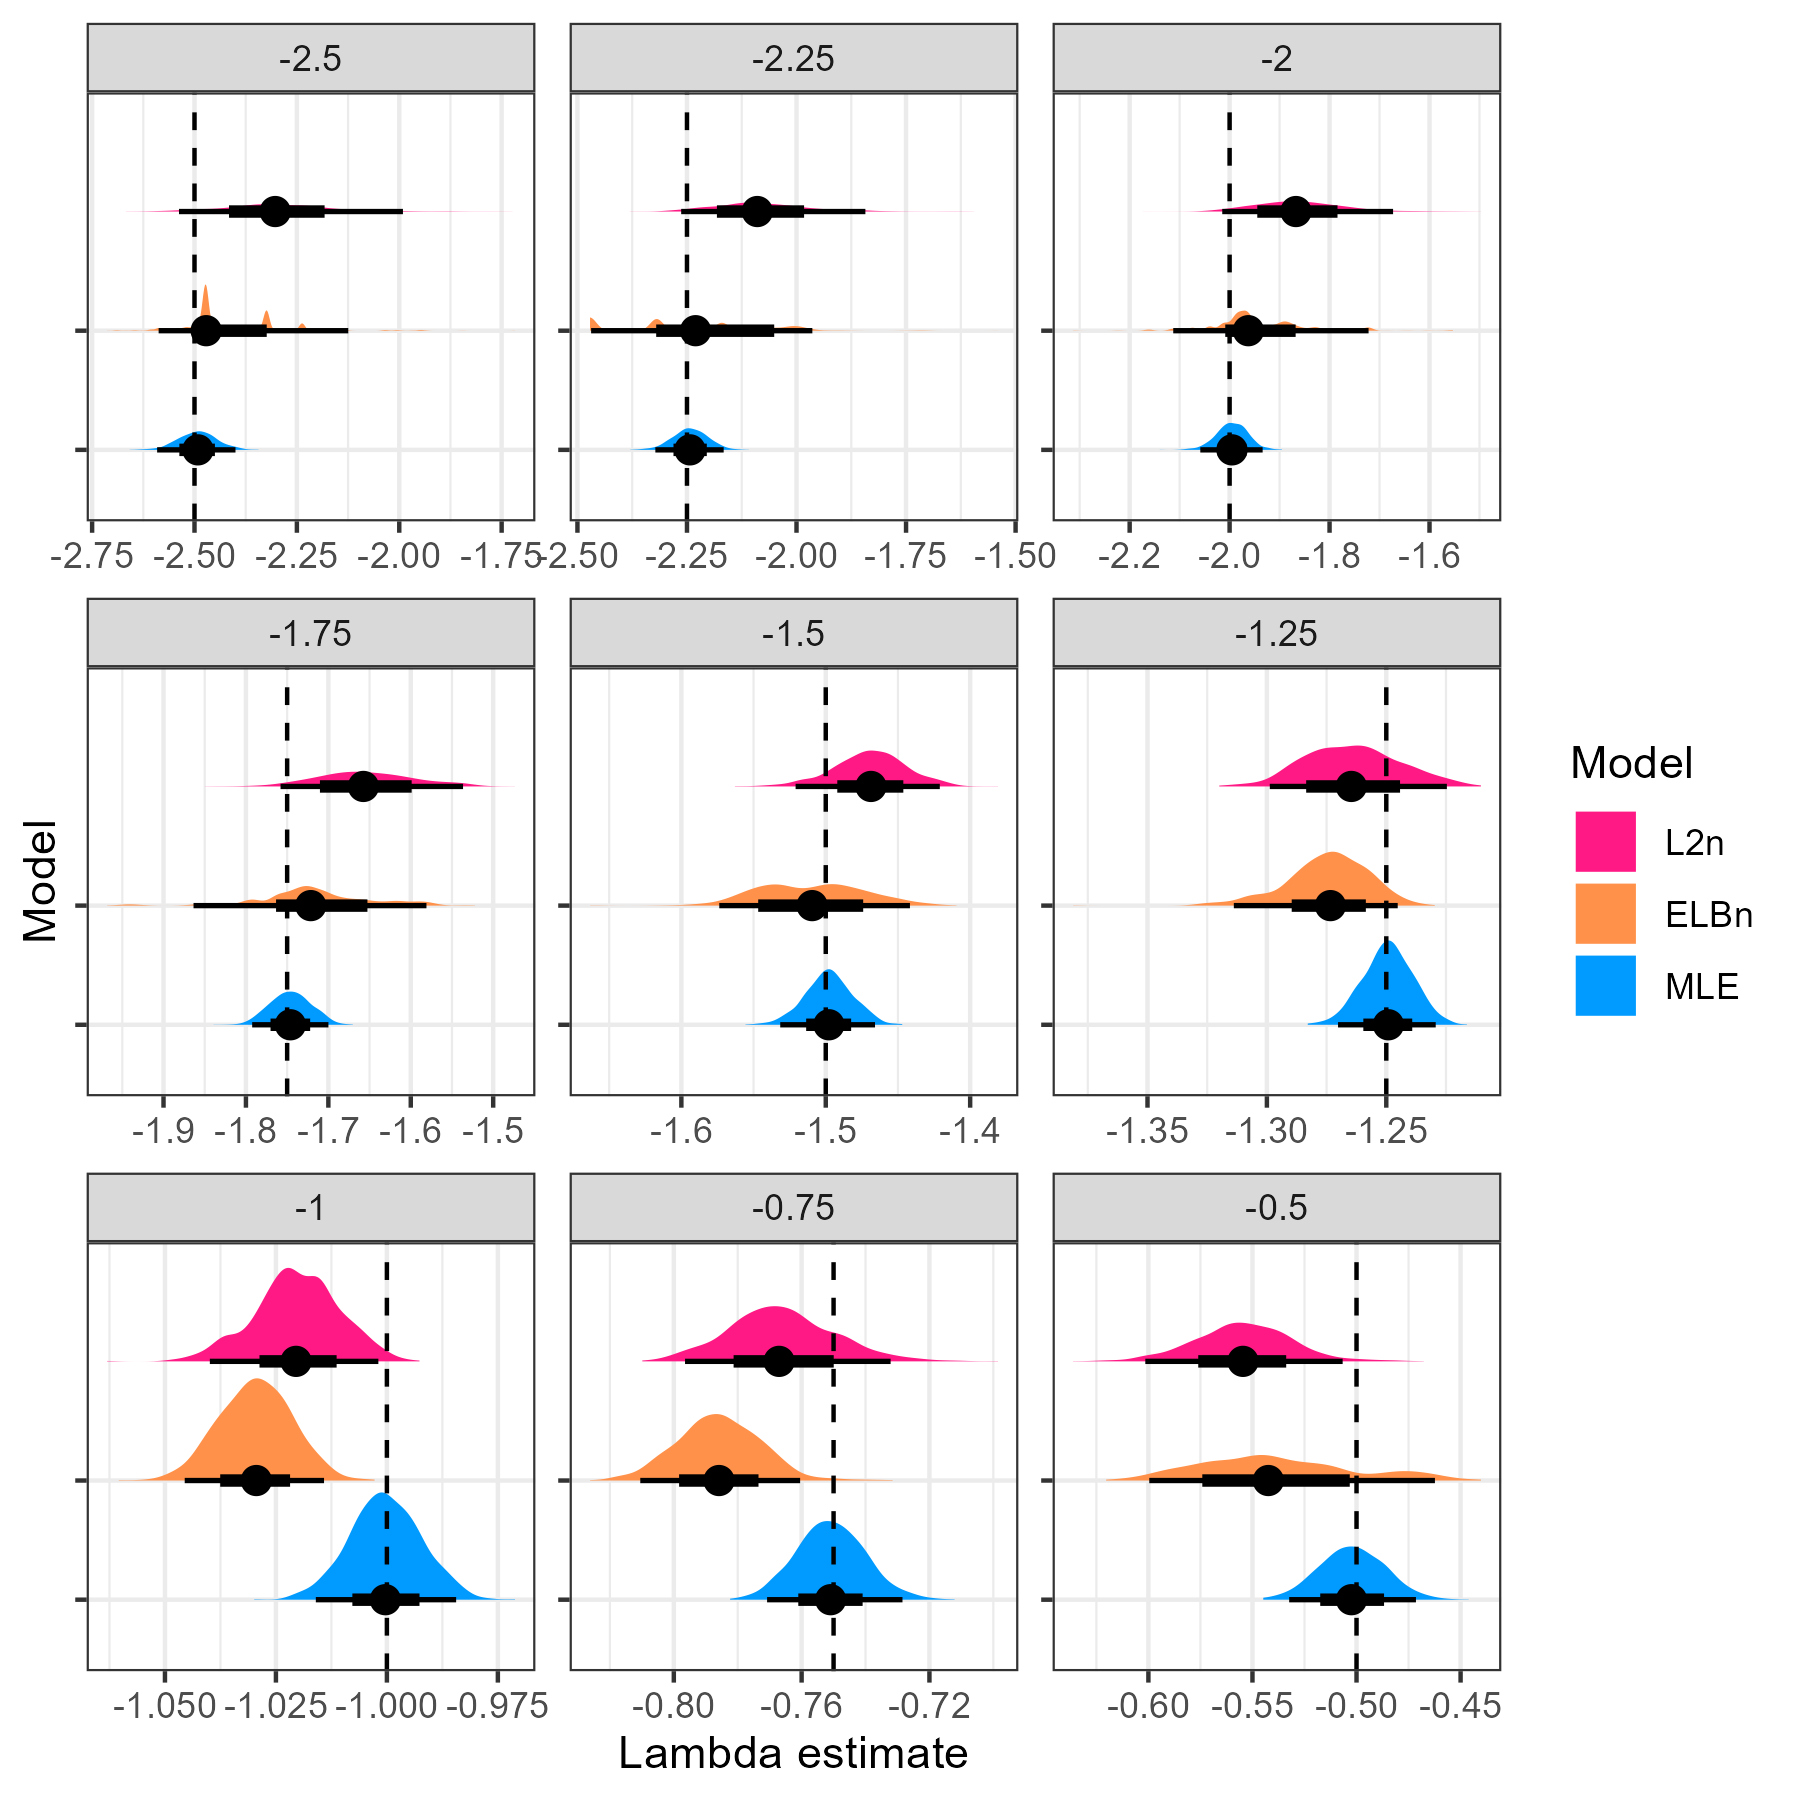
\includegraphics{figures/est_lambda_est_b_density.png}
\caption{Figure 1. Distribution of Lambda estimates by method (color)
from random samples of body sizes from bounded power law distributions
with varying exponents (-2.5, -0.5). The figure is facetted by the known
lambda parameter (facet title) and is also shown as the dashed line in
each facet. Note that the x-axis varies in each facet.}
\end{figure}

\begin{longtable}[]{@{}llrrrr@{}}
\caption{Table 1. Summary of three methods in recapturing the known
values of lambda or the regression slopes simulated in this study.
Performance is determined by comparinged by uncertainty (range of 95\%
CI's) and the absolute distance of the model estimates from the known
estimates (median and sd of the difference). Values are summarized
across all n = 9000 or 6000 simulated datasets. See figures for more
specific comparisons.}\tabularnewline
\toprule
\begin{minipage}[b]{(\columnwidth - 5\tabcolsep) * \real{0.17}}\raggedright
Target\strut
\end{minipage} &
\begin{minipage}[b]{(\columnwidth - 5\tabcolsep) * \real{0.07}}\raggedright
Method\strut
\end{minipage} &
\begin{minipage}[b]{(\columnwidth - 5\tabcolsep) * \real{0.05}}\raggedleft
n\strut
\end{minipage} &
\begin{minipage}[b]{(\columnwidth - 5\tabcolsep) * \real{0.23}}\raggedleft
Median Range of 95\% CI\strut
\end{minipage} &
\begin{minipage}[b]{(\columnwidth - 5\tabcolsep) * \real{0.26}}\raggedleft
Median Absolute Deviation\strut
\end{minipage} &
\begin{minipage}[b]{(\columnwidth - 5\tabcolsep) * \real{0.22}}\raggedleft
SD Absolute Deviation\strut
\end{minipage}\tabularnewline
\midrule
\endfirsthead
\toprule
\begin{minipage}[b]{(\columnwidth - 5\tabcolsep) * \real{0.17}}\raggedright
Target\strut
\end{minipage} &
\begin{minipage}[b]{(\columnwidth - 5\tabcolsep) * \real{0.07}}\raggedright
Method\strut
\end{minipage} &
\begin{minipage}[b]{(\columnwidth - 5\tabcolsep) * \real{0.05}}\raggedleft
n\strut
\end{minipage} &
\begin{minipage}[b]{(\columnwidth - 5\tabcolsep) * \real{0.23}}\raggedleft
Median Range of 95\% CI\strut
\end{minipage} &
\begin{minipage}[b]{(\columnwidth - 5\tabcolsep) * \real{0.26}}\raggedleft
Median Absolute Deviation\strut
\end{minipage} &
\begin{minipage}[b]{(\columnwidth - 5\tabcolsep) * \real{0.22}}\raggedleft
SD Absolute Deviation\strut
\end{minipage}\tabularnewline
\midrule
\endhead
\begin{minipage}[t]{(\columnwidth - 5\tabcolsep) * \real{0.17}}\raggedright
Lambda\strut
\end{minipage} &
\begin{minipage}[t]{(\columnwidth - 5\tabcolsep) * \real{0.07}}\raggedright
MLE\strut
\end{minipage} &
\begin{minipage}[t]{(\columnwidth - 5\tabcolsep) * \real{0.05}}\raggedleft
9000\strut
\end{minipage} &
\begin{minipage}[t]{(\columnwidth - 5\tabcolsep) * \real{0.23}}\raggedleft
0.0661400\strut
\end{minipage} &
\begin{minipage}[t]{(\columnwidth - 5\tabcolsep) * \real{0.26}}\raggedleft
0.0120454\strut
\end{minipage} &
\begin{minipage}[t]{(\columnwidth - 5\tabcolsep) * \real{0.22}}\raggedleft
0.0191500\strut
\end{minipage}\tabularnewline
\begin{minipage}[t]{(\columnwidth - 5\tabcolsep) * \real{0.17}}\raggedright
Lambda\strut
\end{minipage} &
\begin{minipage}[t]{(\columnwidth - 5\tabcolsep) * \real{0.07}}\raggedright
NAS\strut
\end{minipage} &
\begin{minipage}[t]{(\columnwidth - 5\tabcolsep) * \real{0.05}}\raggedleft
9000\strut
\end{minipage} &
\begin{minipage}[t]{(\columnwidth - 5\tabcolsep) * \real{0.23}}\raggedleft
0.1335267\strut
\end{minipage} &
\begin{minipage}[t]{(\columnwidth - 5\tabcolsep) * \real{0.26}}\raggedleft
0.0460093\strut
\end{minipage} &
\begin{minipage}[t]{(\columnwidth - 5\tabcolsep) * \real{0.22}}\raggedleft
0.0929513\strut
\end{minipage}\tabularnewline
\begin{minipage}[t]{(\columnwidth - 5\tabcolsep) * \real{0.17}}\raggedright
Lambda\strut
\end{minipage} &
\begin{minipage}[t]{(\columnwidth - 5\tabcolsep) * \real{0.07}}\raggedright
ELBn\strut
\end{minipage} &
\begin{minipage}[t]{(\columnwidth - 5\tabcolsep) * \real{0.05}}\raggedleft
8579\strut
\end{minipage} &
\begin{minipage}[t]{(\columnwidth - 5\tabcolsep) * \real{0.23}}\raggedleft
0.1672598\strut
\end{minipage} &
\begin{minipage}[t]{(\columnwidth - 5\tabcolsep) * \real{0.26}}\raggedleft
0.0350186\strut
\end{minipage} &
\begin{minipage}[t]{(\columnwidth - 5\tabcolsep) * \real{0.22}}\raggedleft
0.0675122\strut
\end{minipage}\tabularnewline
\begin{minipage}[t]{(\columnwidth - 5\tabcolsep) * \real{0.17}}\raggedright
Regression Slope\strut
\end{minipage} &
\begin{minipage}[t]{(\columnwidth - 5\tabcolsep) * \real{0.07}}\raggedright
MLE\strut
\end{minipage} &
\begin{minipage}[t]{(\columnwidth - 5\tabcolsep) * \real{0.05}}\raggedleft
6000\strut
\end{minipage} &
\begin{minipage}[t]{(\columnwidth - 5\tabcolsep) * \real{0.23}}\raggedleft
0.0382185\strut
\end{minipage} &
\begin{minipage}[t]{(\columnwidth - 5\tabcolsep) * \real{0.26}}\raggedleft
0.0086982\strut
\end{minipage} &
\begin{minipage}[t]{(\columnwidth - 5\tabcolsep) * \real{0.22}}\raggedleft
0.0089766\strut
\end{minipage}\tabularnewline
\begin{minipage}[t]{(\columnwidth - 5\tabcolsep) * \real{0.17}}\raggedright
Regression Slope\strut
\end{minipage} &
\begin{minipage}[t]{(\columnwidth - 5\tabcolsep) * \real{0.07}}\raggedright
NAS\strut
\end{minipage} &
\begin{minipage}[t]{(\columnwidth - 5\tabcolsep) * \real{0.05}}\raggedleft
6000\strut
\end{minipage} &
\begin{minipage}[t]{(\columnwidth - 5\tabcolsep) * \real{0.23}}\raggedleft
0.0799201\strut
\end{minipage} &
\begin{minipage}[t]{(\columnwidth - 5\tabcolsep) * \real{0.26}}\raggedleft
0.0513434\strut
\end{minipage} &
\begin{minipage}[t]{(\columnwidth - 5\tabcolsep) * \real{0.22}}\raggedleft
0.0442020\strut
\end{minipage}\tabularnewline
\begin{minipage}[t]{(\columnwidth - 5\tabcolsep) * \real{0.17}}\raggedright
Regression Slope\strut
\end{minipage} &
\begin{minipage}[t]{(\columnwidth - 5\tabcolsep) * \real{0.07}}\raggedright
ELBn\strut
\end{minipage} &
\begin{minipage}[t]{(\columnwidth - 5\tabcolsep) * \real{0.05}}\raggedleft
6000\strut
\end{minipage} &
\begin{minipage}[t]{(\columnwidth - 5\tabcolsep) * \real{0.23}}\raggedleft
0.0923495\strut
\end{minipage} &
\begin{minipage}[t]{(\columnwidth - 5\tabcolsep) * \real{0.26}}\raggedleft
0.0300186\strut
\end{minipage} &
\begin{minipage}[t]{(\columnwidth - 5\tabcolsep) * \real{0.22}}\raggedleft
0.0353218\strut
\end{minipage}\tabularnewline
\bottomrule
\end{longtable}

Furthermore, the binning methods systematically over estimated steep
size spectra relationships (\(\lambda = ~\sim-2.5~to-1.5\), Figure 2),
and slightly underestimated shallow size spectra relationships
(\(\lambda = ~\sim-0.5\)). This finding was more pronounced in the NAS
method compared with the ELBn method.

\begin{figure}
\centering
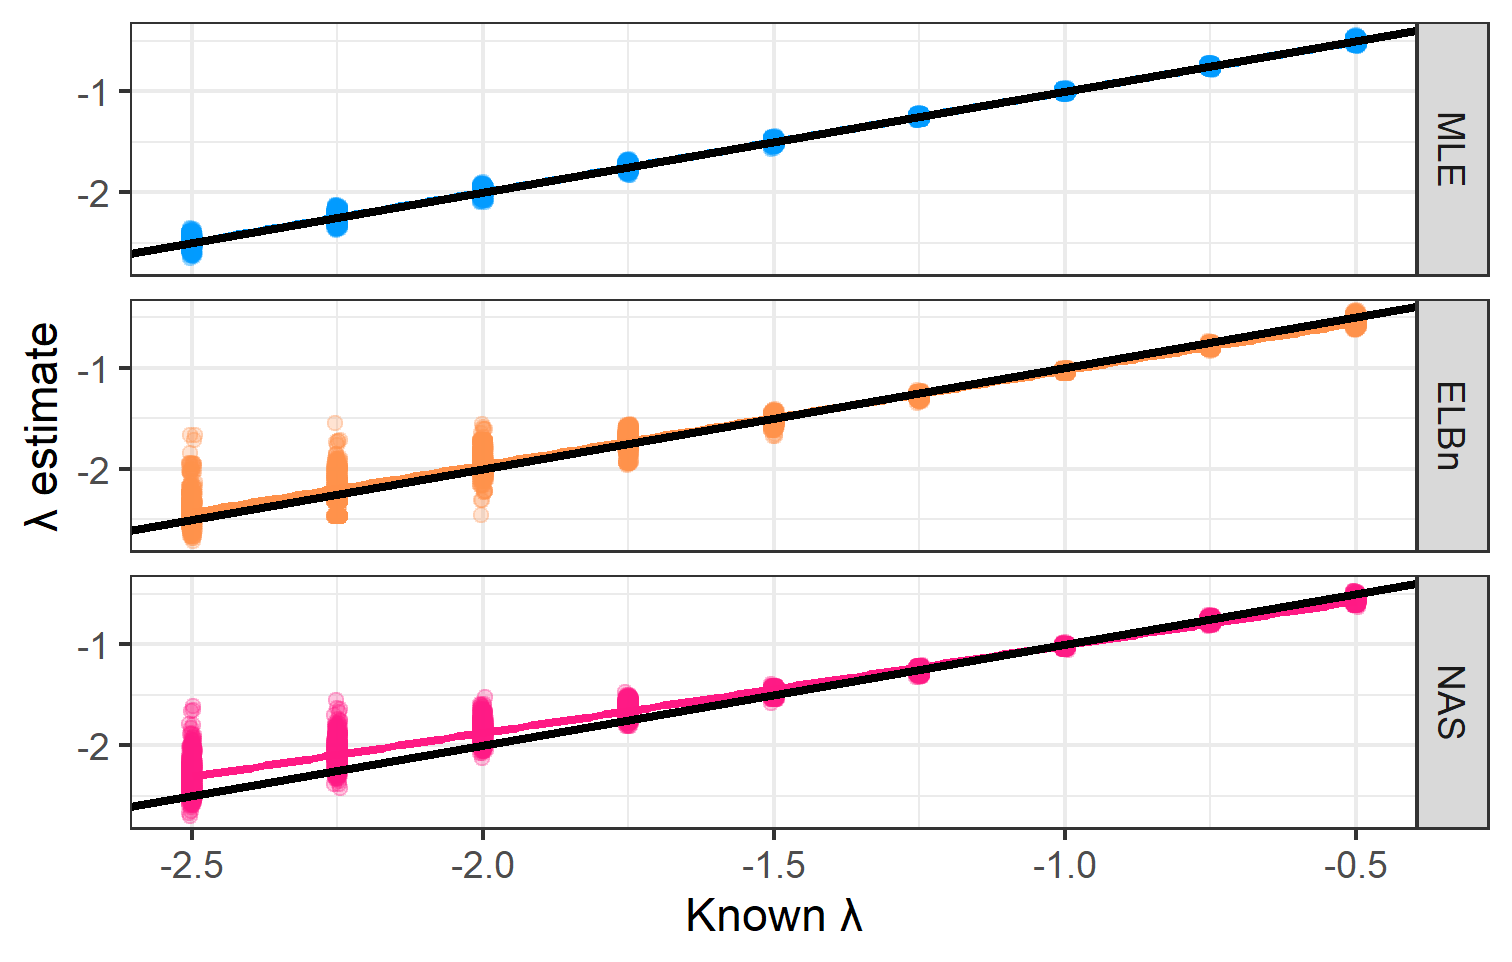
\includegraphics{figures/known_est_b_line.png}
\caption{Figure 2. Plot of the known and estimated lambda from different
methods (color). The dashed line is the 1:1 line, and almost perfectly
matches the MLE (Blue) estimate. The two binning method cross the 1:1
line, meaning they systematically underestimate shallow lambdas, and
over estimate steeper lambdas.}
\end{figure}

\hypertarget{relationship-across-the-hypothetical-environmental-gradient}{%
\subsection{Relationship across the hypothetical environmental
gradient}\label{relationship-across-the-hypothetical-environmental-gradient}}

\hypertarget{lambda-windows}{%
\subsubsection{\texorpdfstring{\(\lambda\)
``windows''}{\textbackslash lambda ``windows''}}\label{lambda-windows}}

Because of the different performance of the two binning methods at steep
and shallow values of lambdas, we first investigated how well the
methods capture a known relationship of \(\beta_{env} = -0.5\) across a
hypothetical environmental gradient. The lambda ``windows'' are steep
(-2.5, -1.5), medium (-2, -1) and shallow (-1.5, -0.5).

\begin{figure}
\centering
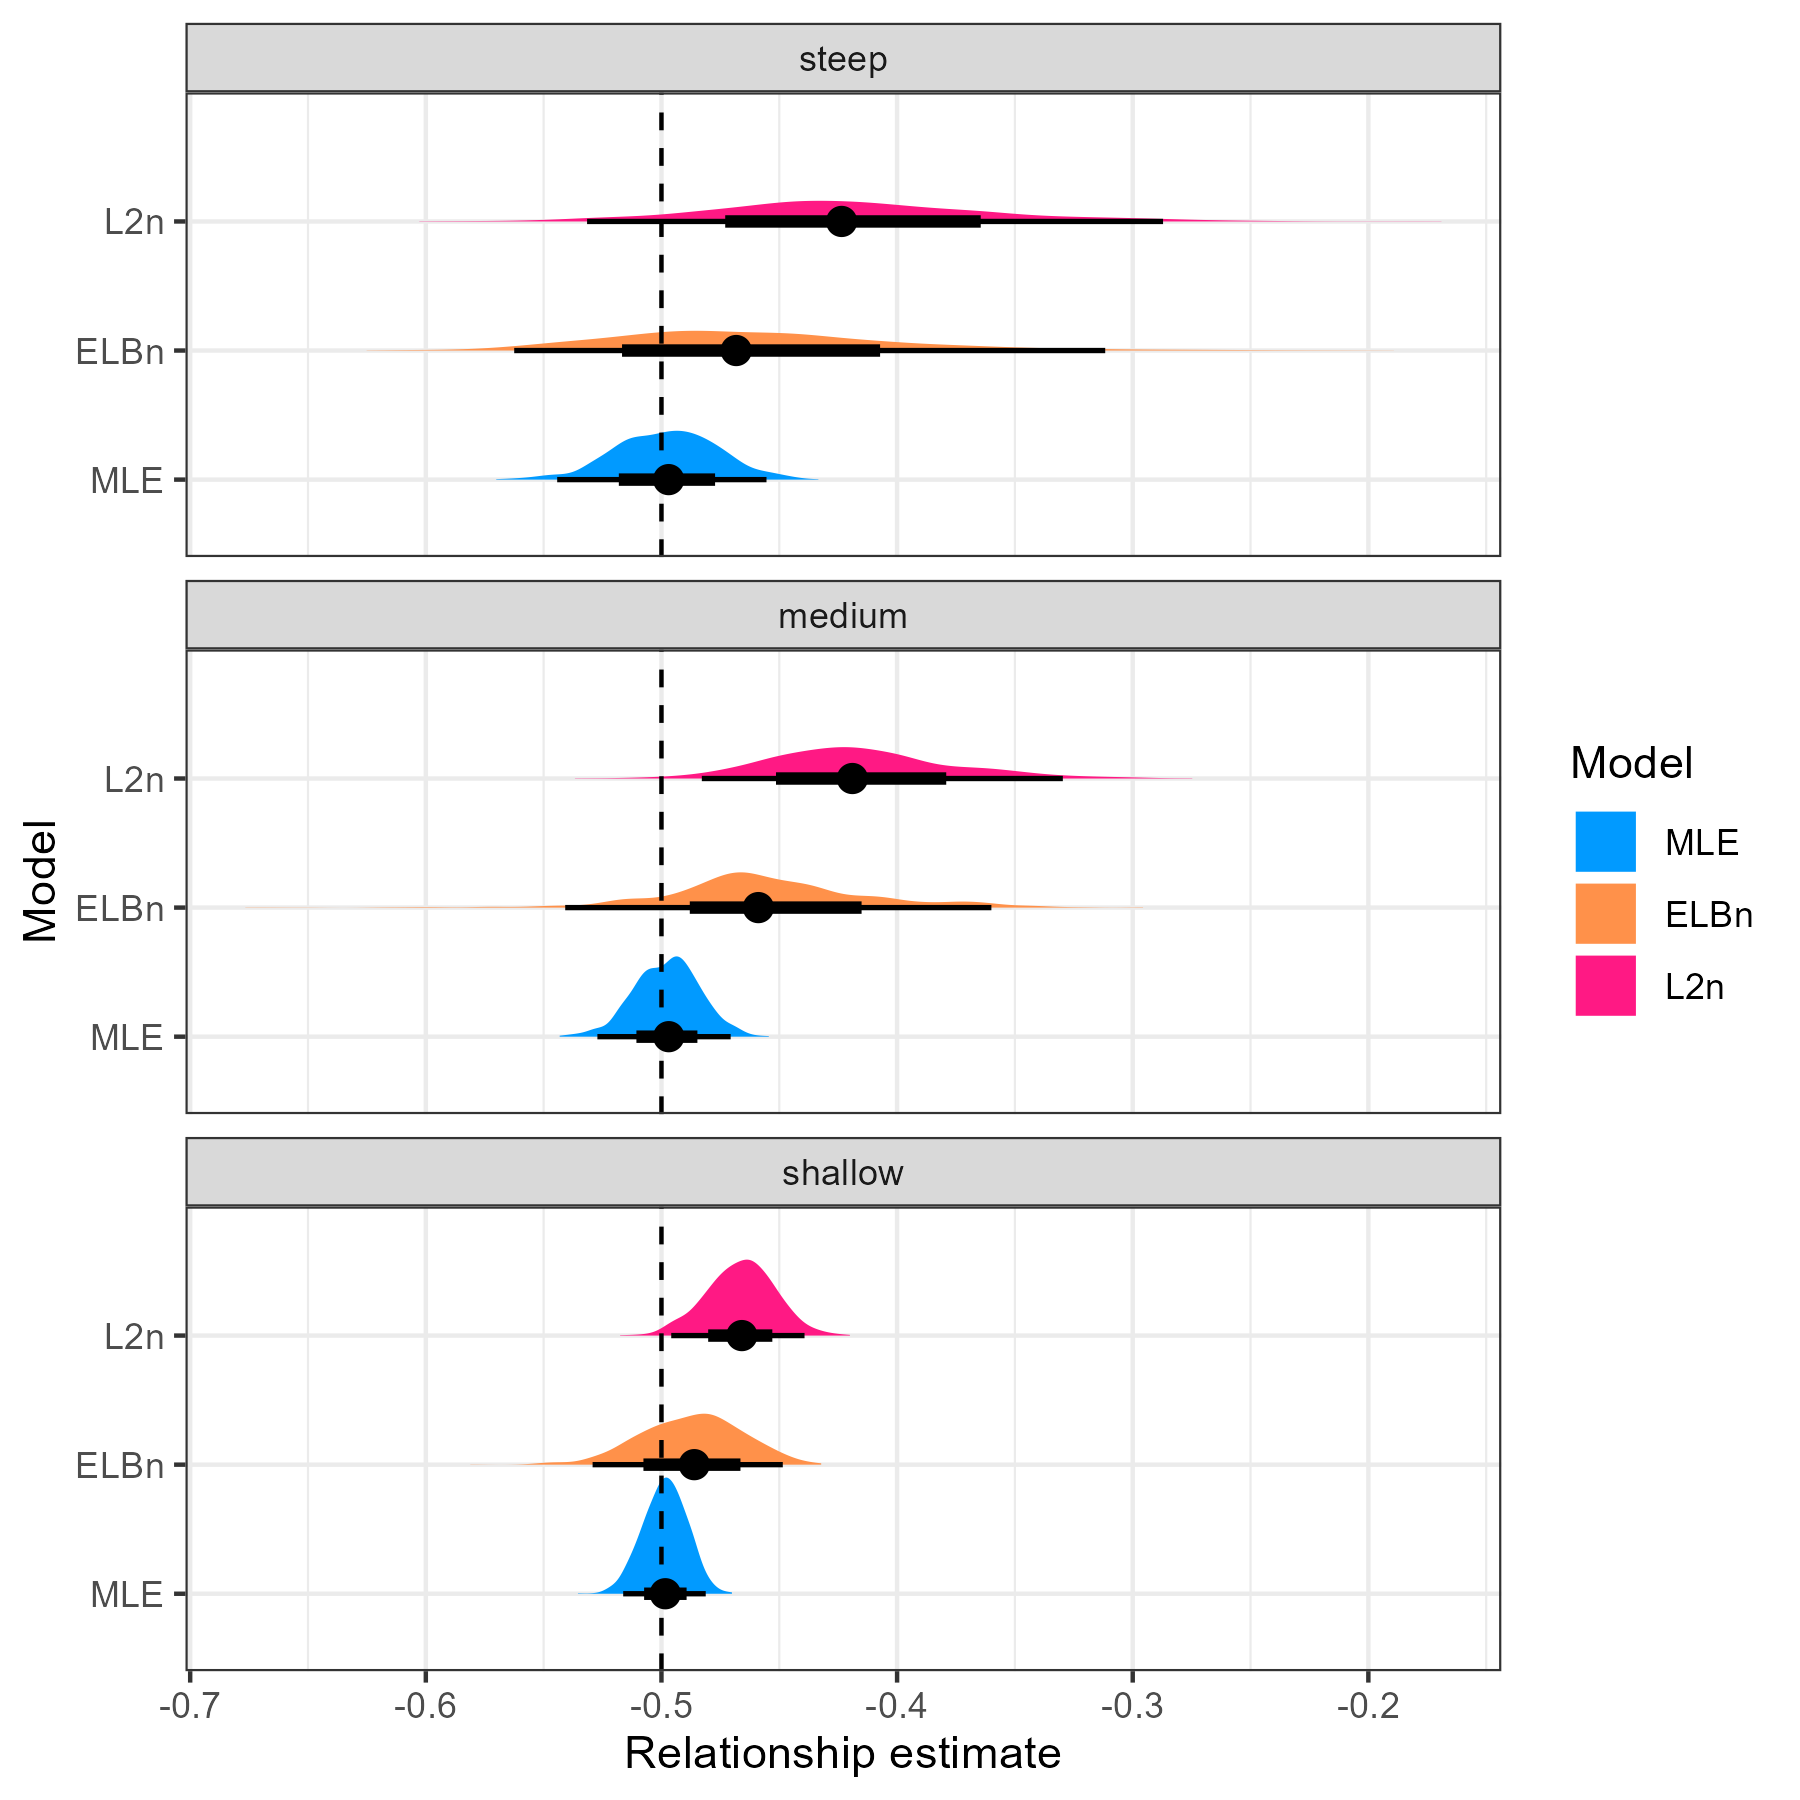
\includegraphics{figures/lambda_angle_plot.png}
\caption{Figure 3. Distribution of relationship estimates
(\(beta_{env}\)) in three different ``windows'' of lambda values. The
dashed vertical line is the known relationship value of -0.5.}
\end{figure}

The MLE method (Figure 3, blue) recaptured the known slope value in each
of the ``windows.'' with median absolute deviation of
\textasciitilde0.01 units (Table 1). By contrast, the binning methods
systematically overestimated the known slope (Figure 3), with median
absolute deviations \textgreater4 times higher than the MLE. Similarly,
uncertainty in the slope estimates derived from binning methods was
twice that of the uncertainty in the MLE method (Table 1).

\hypertarget{varying-the-known-relationship}{%
\subsubsection{Varying the Known
Relationship}\label{varying-the-known-relationship}}

All methods recaptured the correct sign of the slopes, yielding
qualitative consistency (Figure 4). However, the binning methods again
systematically underestimated the true value of the slope by
\textasciitilde0.05 units (Figure 5). Likewise, uncertainty in the slope
estimates was always greater in the binning methods, with the width of
the distributions increases with stronger relationships across a
hypothetical gradient. By comparison, the MLE showed no evidence of bias
and was always centered at the known value with relatively narrow
variation.

\begin{figure}
\centering
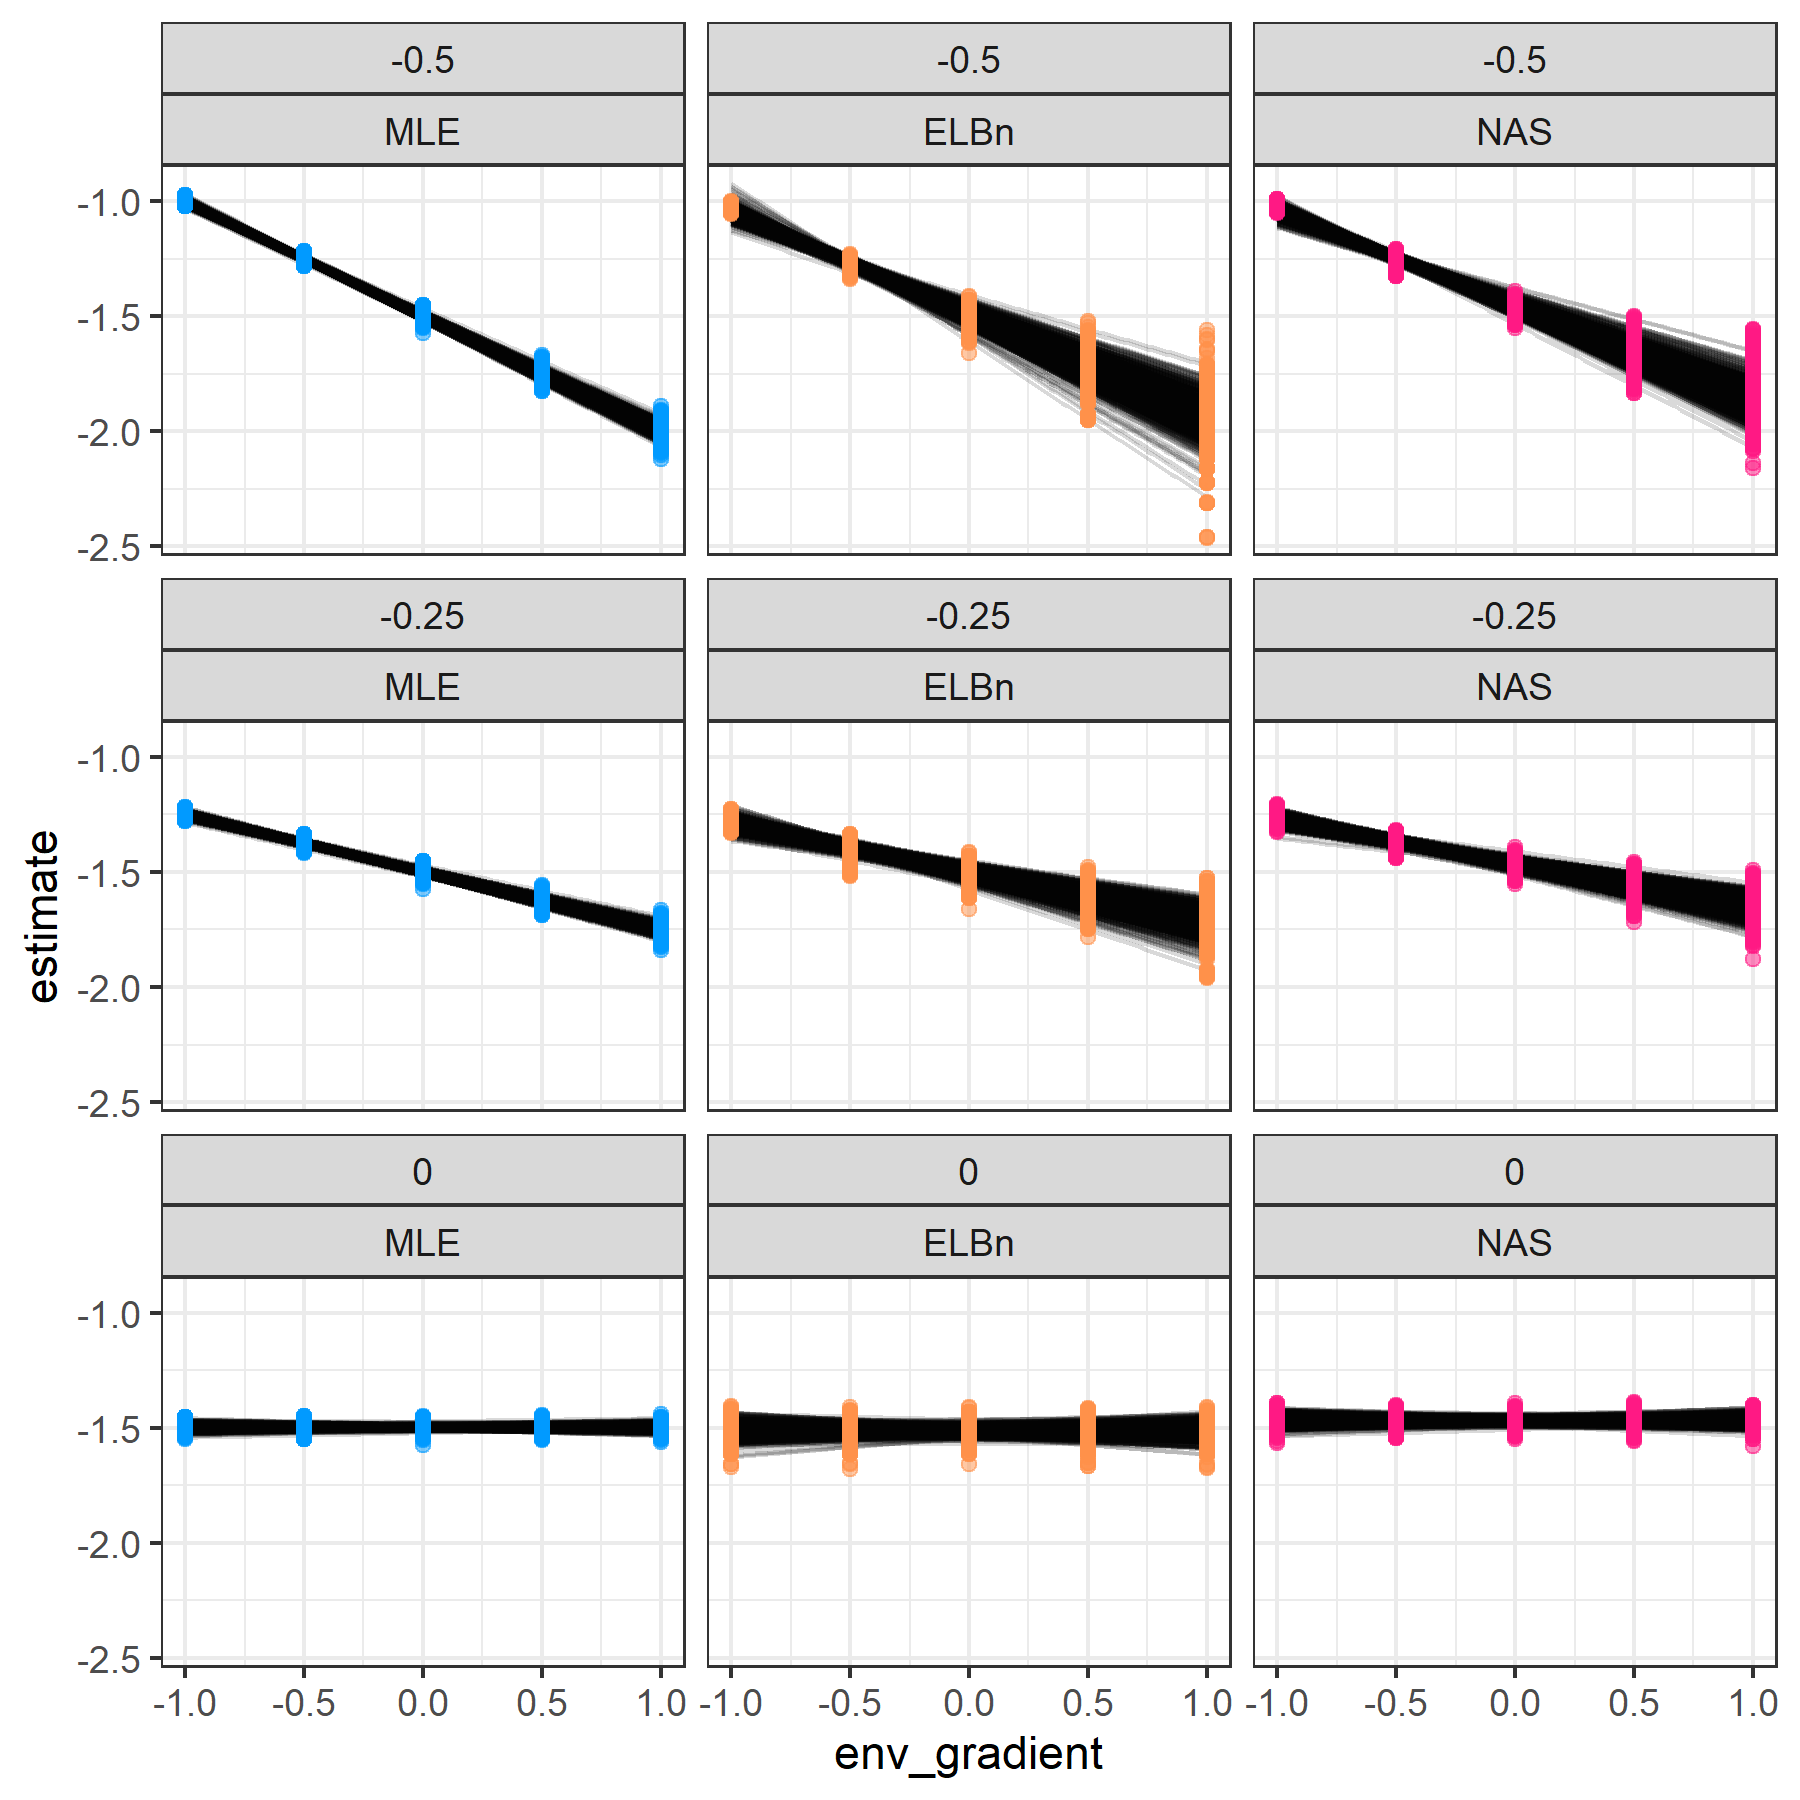
\includegraphics{figures/vary_beta_plot.png}
\caption{Figure 4. Individual regressions for each rep (N = 1000) and
method (columns) for three different known relationship values (rows
from bottom to top): 0, 0.25, and 0.5}
\end{figure}

\begin{figure}
\centering
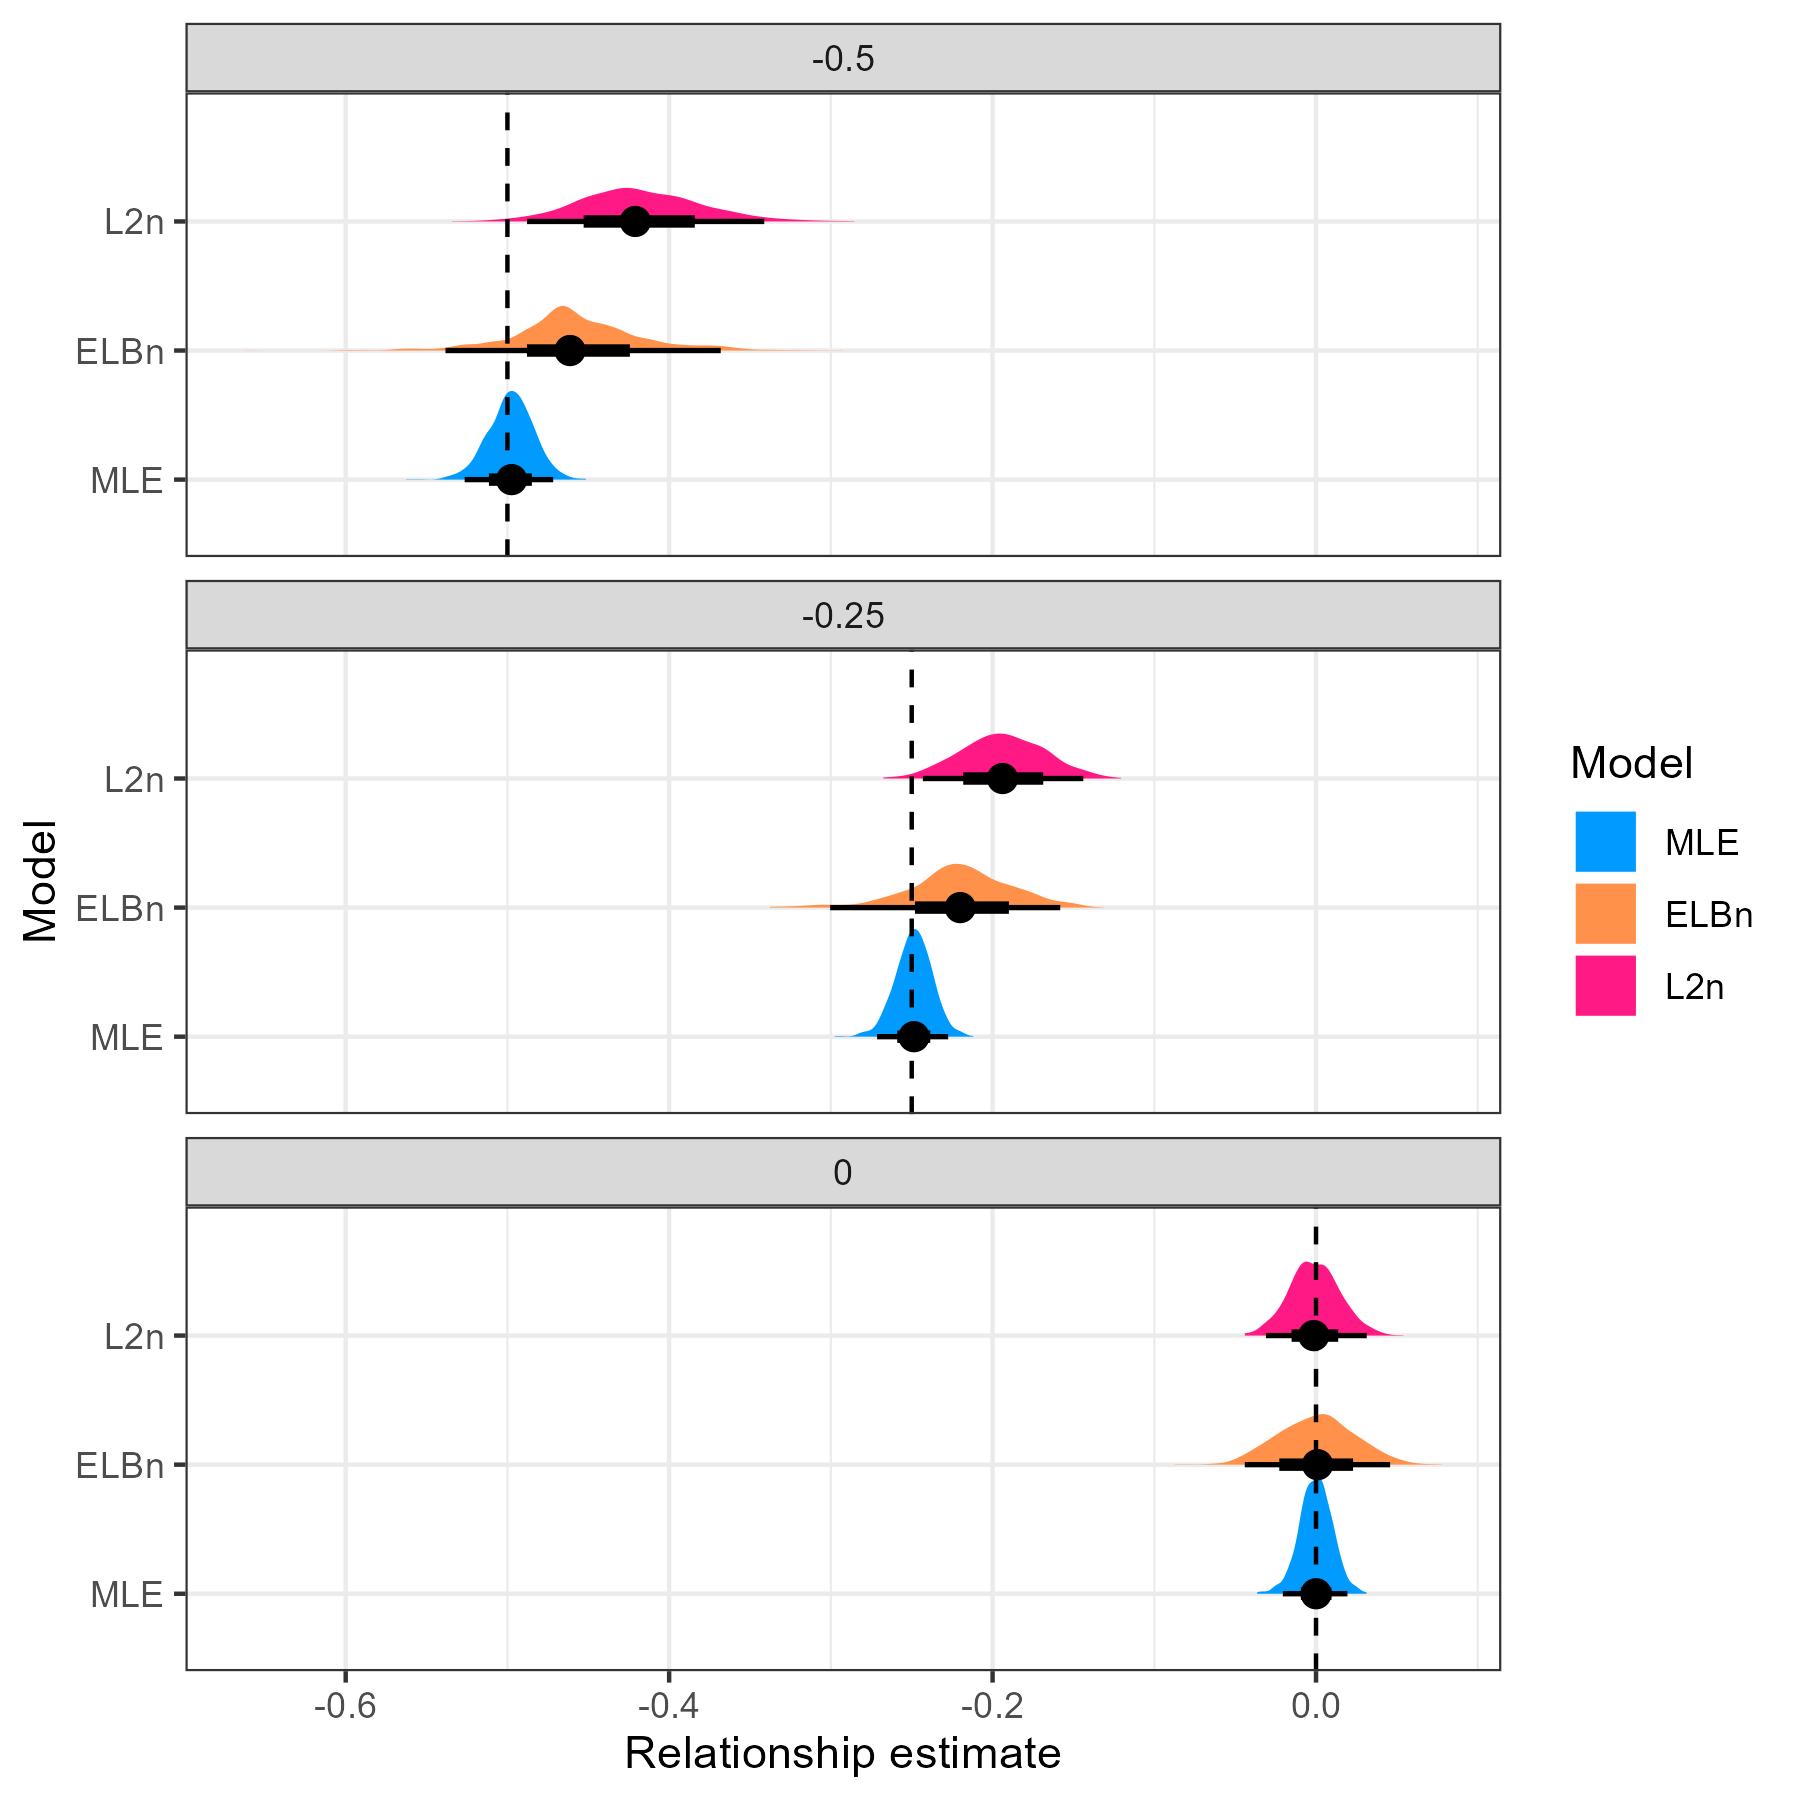
\includegraphics{figures/vary_beta_density_plot.png}
\caption{Figure 5. Distribution of relationship estimates (beta\_1) when
estimating from different known relationships}
\end{figure}

\hypertarget{empirical-data-1}{%
\subsection{Empirical data}\label{empirical-data-1}}

Both empirical data sets yielded similar results to the simulated data;
the direction of the coefficients (i.e., \(\beta_1\) coefficients) were
the same among methods, with positive slopes across the AMD gradient
(Fig. 6A) and negative slopes across the temperature gradient. However,
the magnitude of change differed between methods. The AMD slopes ranged
from \textasciitilde0.62 with MLE to \textasciitilde0.78 with NAS
(Figure 6b), while temperature slopes ranged from -0.0058 with MLE to
-0.0019 with ELBn (Figure 6d). As with simulated data, slope uncertainty
(\(\pm\) 1 SD) was larger in the binning methods, particularly the ELBn
method (Fig. 6B). Likewise, the size spectra parameters consistently
increase (become steeper) with increasing temperature across the NEON
sites (Fig. 6C).

\newpage

\begin{figure}
\centering
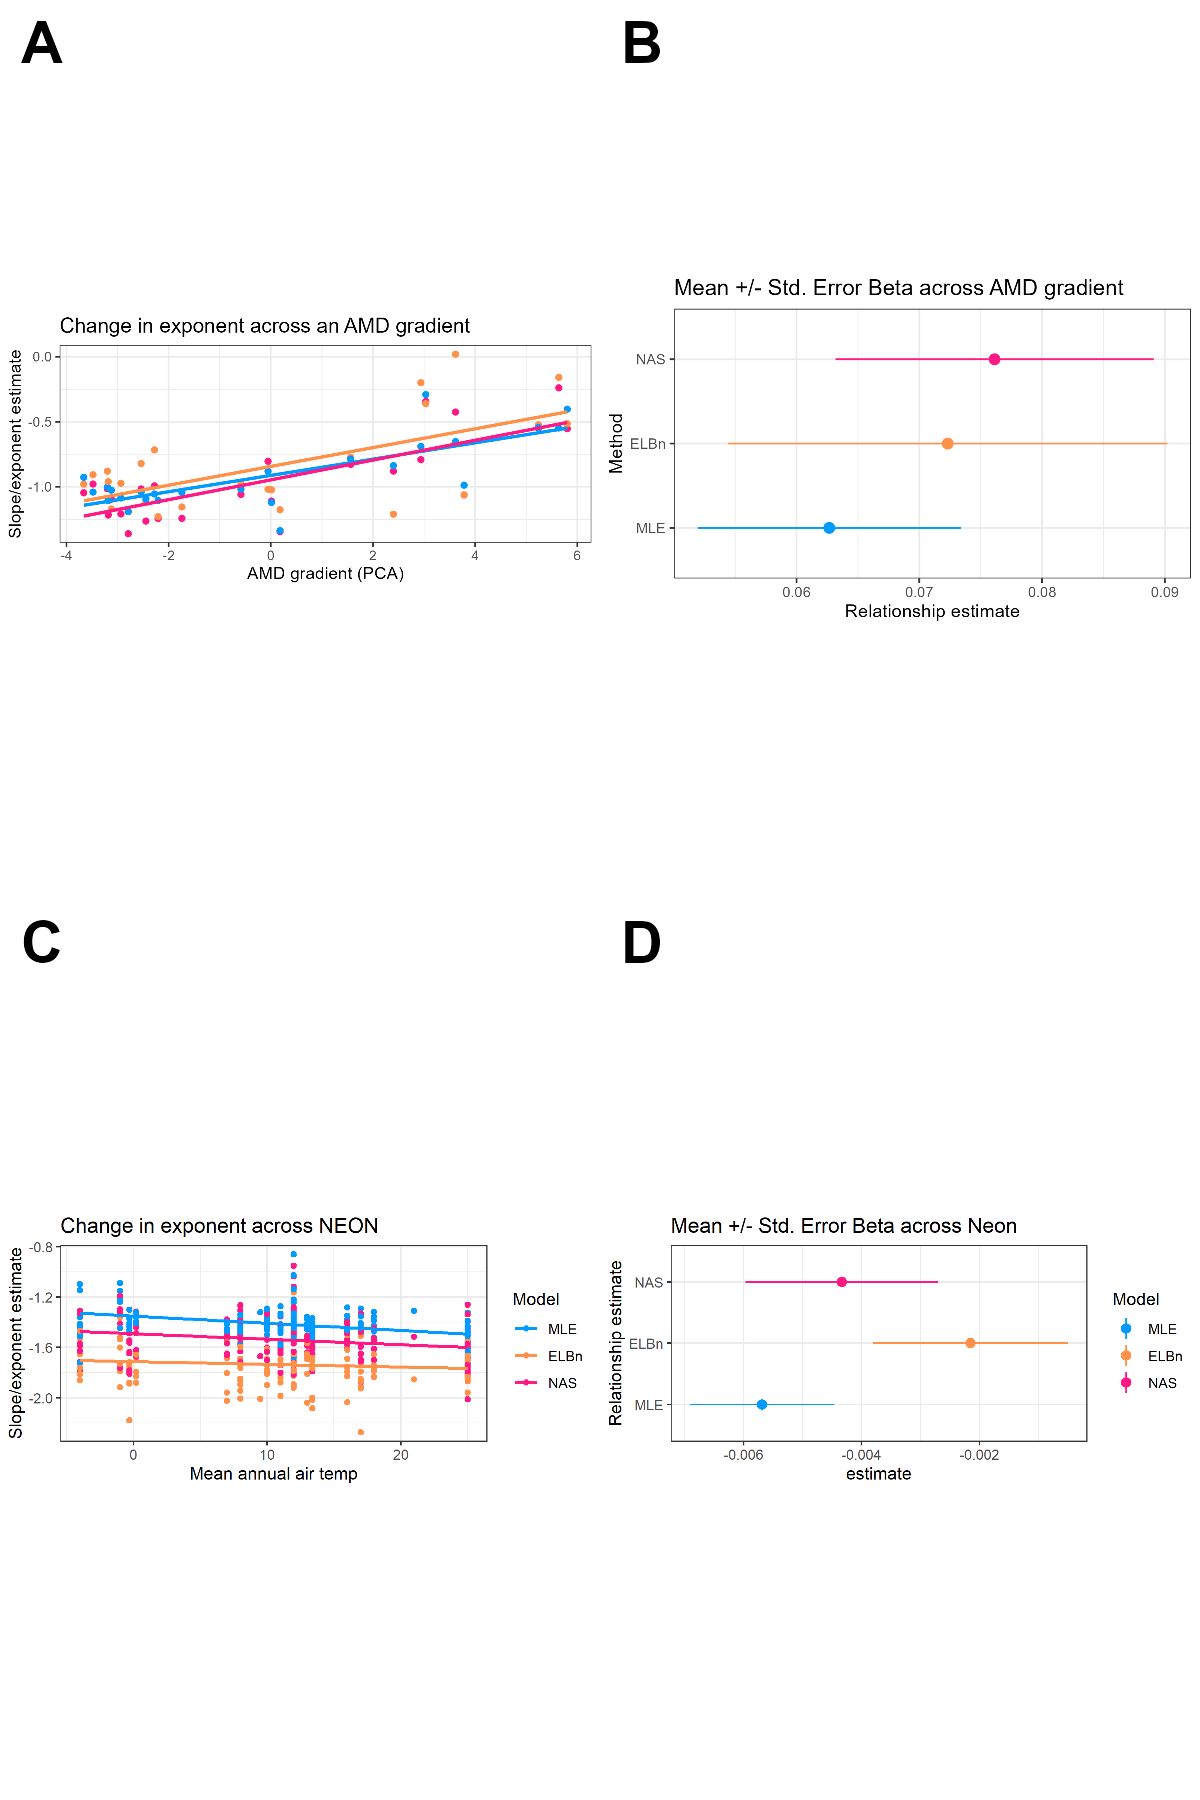
\includegraphics{figures/empirical_combined.png}
\caption{Figure 6. of empirical data estimates. All of the methods
estimate the same sign of the relationship, but the estimates from the
binning methods are generally greater than the MLE estimates.}
\end{figure}

\newpage

\hypertarget{discussion}{%
\section{Discussion}\label{discussion}}

The relationship between body size and abundance has been extensively
studied in a wide range of taxa inhabiting both terrestrial and aquatic
ecosystems (reviewed by {[}Brown (1995); GastonBlackburn2000; White et
al. (2007){]}). Empirical data shows generally consistent patterns and
can be explained by the metabolic theory of ecology (Brown et al. 2004).
Measuring parameters describing the decline in abundance with increasing
body size in communities is being done with increasing frequency across
ecology. Previous work has investigated the accuracy and inherent biases
associated with different estimation methods (White et al. 2007, Edwards
et al. 2017, Edwards et al. 2020). However, how these inaccuracies and
biases compound across environmental gradients remains uncertain, making
it difficult to detect variation in size spectra parameters across
environmental gradients with confidence. The most important outcome of
our work is that binning methods not only generate biased \(\lambda\)
values for individual data sets, but that bias carries over to affect
the parameters of subsequent regressions that use those \(\lambda\)'s as
response variables. This makes it challenging to understand how
\(\lambda\) varies in response to environmental gradients if binning is
used to estimate size spectra exponents.

Binning methods are easy to use and interpret, which most likely
accounts for their wide use in ecological studies. However, aggregating
individuals into logarithmic bins removes a large source of the
variation within the data by collapsing body size variation into a
single value within each bin. For example, all individuals placed into a
bin that ranges from 2-4 grams of mass are all treated as having a mass
of 3 grams, the midpoint of that bin. Likewise, a single abundance value
is taken for each bin, despite that fact that there is almost certainly
variation in the abundance of individuals that weigh \textasciitilde2,
\textasciitilde3, or \textasciitilde4 grams. Moreover, the number of
bins that can be produced by any dataset is limited most often to less
than six. That means a subsequent log-log regression used to estimate
\(\lambda\) would contains n = 6 data points, even though there likely
100's or 1000's of individual body sizes available in a typical body
size data set. By homogenizing the data in this way, binning methods
produce noisier results than MLE, since binning is akin to deleting
information that the model could otherwise use. By contrast, the MLE
uses all the individual body size data to directly estimate \(\lambda\),
meaning that it not only produces more accurate estimates, but does so
with less certainty than binning, even when the underlying data sets are
identical.

The error in estimating individual \(\lambda\)'s was compounded when
estimating linear models with those \(\lambda\)'s as response variables.
The MLE method also resulted in the most accurate \(\beta_{env}\)
estimates. Furthermore, variation around the estimate was always
smallest with the MLE method.

Although there were differences in magnitude of the empirical
relationship coefficients, they were generally in the correct direction
and of a similar magnitude. This suggests that previously reported
significant changes in size spectra parameters across environmental
gradients and in experimental manipulations are plausible. Given that
all of the data within a study is treated identically, the over all
change in size spectra parameters is likely reasonable. However, the
biases and inconsistencies in relationship estimates presented here
suggest that it would be difficult if not impossible to directly compare
the relative changes across different published studies which use
different methods.

The publication of individual body size data with future studies of size
spectra would greatly aid in our ability to generalize changes to this
fundamental aspect of community organization across spatiotemporal
scales and in response to environmental conditions.

\hypertarget{concluding-remarks}{%
\subsection{Concluding Remarks}\label{concluding-remarks}}

The MLE method outperformed both of the binning methods under nearly any
measure. With the publication of the \emph{sizespectra} package (2017),
producing MLE estimates of size spectra parameters is a relatively easy
task. Therefore, we recommend using it in all future studies of size
spectra relationships rather than binning.

We reiterate the recommendations of (2017) to estimate size spectra
relationships using MLE methods due to their superior performance in
nearly every context. Furthermore, we strongly encourage authors to
publish individual size data whenever possible. This will allow for the
consistent re-analysis of existing data sets as methodologies develop
and improve. This will aid in the ability for size spectra work to be
synthesized between research groups and across scales.

\newpage

\hypertarget{references}{%
\section{References}\label{references}}

\hypertarget{refs}{}
\begin{CSLReferences}{1}{0}
\leavevmode\hypertarget{ref-Andersen2006a}{}%
Andersen, K. H., and J. E. Beyer. 2006. Asymptotic {Size Determines
Species Abundance} in the {Marine Size Spectrum}. The American
Naturalist 168:54--61.

\leavevmode\hypertarget{ref-brown1995}{}%
Brown, J. H. 1995. Macroecology. {University of Chicago Press},
{Chicago, IL}.

\leavevmode\hypertarget{ref-Brown2004}{}%
Brown, J. H., J. F. Gillooly, A. P. Allen, V. M. Savage, and G. B. West.
2004. Toward a metabolic theory of ecology. Ecology 85:1771--1789.

\leavevmode\hypertarget{ref-Damuth1981}{}%
Damuth, J. 1981. Population density and body size in mammals. Nature
290:699--700.

\leavevmode\hypertarget{ref-Damuth1991}{}%
Damuth, J. 1991. Of size and abundance. Nature 351:268--269.

\leavevmode\hypertarget{ref-Damuth1998}{}%
Damuth, J. D. 1998. Common rules for animals and plants. Nature
395:115--116.

\leavevmode\hypertarget{ref-dossena2012}{}%
Dossena, M., G. Yvon-Durocher, J. Grey, J. M. Montoya, D. M. Perkins, M.
Trimmer, and G. Woodward. 2012. Warming alters community size structure
and ecosystem functioning. Proceedings of the Royal Society B
279:3011--3019.

\leavevmode\hypertarget{ref-edwards2020}{}%
Edwards, A. M., J. Robinson, J. Blanchard, J. Baum, and M. Plank. 2020.
Accounting for the bin structure of data removes bias when fitting size
spectra. Marine Ecology Progress Series 636:19--33.

\leavevmode\hypertarget{ref-edwards2017}{}%
Edwards, A. M., J. Robinson, M. Plank, J. Baum, and J. Blanchard. 2017.
Testing and recommending methods for fitting size spectra to data.
Methods in Ecology and Evolution 8:57--67.

\leavevmode\hypertarget{ref-evans2022}{}%
Evans, T. M., Z. S. Feiner, L. G. Rudstam, D. M. Mason, J. M. Watkins,
E. D. Reavie, A. E. Scofield, L. E. Burlakova, A. Y. Karatayev, and W.
G. Sprules. 2022. Size spectra analysis of a decade of {Laurentian Great
Lakes} data. Canadian Journal of Fisheries and Aquatic Sciences
79:183--194.

\leavevmode\hypertarget{ref-jennings2004}{}%
Jennings, S., and J. L. Blanchard. 2004. Fish abundance with no fishing:
Predictions based on macroecological theory. Journal of Animal Ecology
73:632--642.

\leavevmode\hypertarget{ref-Jennings2002}{}%
Jennings, S., K. J. Warr, and S. Mackinson. 2002. Use of size-based
production and stable isotope analyses to predict trophic transfer
efficiencies and predator-prey body mass ratios in food webs. Marine
Ecology Progress Series 240:11--20.

\leavevmode\hypertarget{ref-martinez2016}{}%
Martínez, A., A. Larrañaga, A. Miguélez, G. Yvon-Durocher, and J. Pozo.
2016. Land use change affects macroinvertebrate community size spectrum
in streams: The case of {Pinus} radiata plantations. Freshwater Biology
61:69--79.

\leavevmode\hypertarget{ref-mcgarvey2018}{}%
McGarvey, D. J., and A. J. Kirk. 2018. Seasonal comparison of
community-level size-spectra in southern coalfield streams of {West
Virginia} ({USA}). Hydrobiologia 809:65--77.

\leavevmode\hypertarget{ref-NEON_Inverts2022}{}%
National Ecological Observatory Network (NEON). 2022. Macroinvertebrate
collection ({DP1}.20120.001). {National Ecological Observatory Network
(NEON)}.

\leavevmode\hypertarget{ref-Nee1991}{}%
Nee, S., A. F. Read, J. J. D. Greenwood, and P. H. Harvey. 1991. The
relationship between abundance and body size in {British} birds. Nature
351:312--313.

\leavevmode\hypertarget{ref-perkins2018}{}%
Perkins, D. M., I. Durance, F. K. Edwards, J. Grey, A. G. Hildrew, M.
Jackson, J. I. Jones, R. B. Lauridsen, K. Layer-Dobra, M. S. A.
Thompson, and G. Woodward. 2018. Bending the rules: Exploitation of
allochthonous resources by a top-predator modifies size-abundance
scaling in stream food webs. Ecology Letters.

\leavevmode\hypertarget{ref-Petchey2010}{}%
Petchey, O. L., and A. Belgrano. 2010. Body-size distributions and
size-spectra: Universal indicators of ecological status? Biology Letters
6:434--437.

\leavevmode\hypertarget{ref-pomeranz2022}{}%
Pomeranz, J. P. F., J. R. Junker, and J. S. Wesner. 2022. Individual
size distributions across {North American} streams vary with local
temperature. Global Change Biology 28:848--858.

\leavevmode\hypertarget{ref-pomeranz2019}{}%
Pomeranz, J. P. F., H. J. Warburton, and J. S. Harding. 2019a.
Anthropogenic mining alters macroinvertebrate size spectra in streams.
Freshwater Biology 64:81--92.

\leavevmode\hypertarget{ref-Pomeranz2019}{}%
Pomeranz, J. P. F., H. J. Warburton, and J. S. Harding. 2019b. Data
from: {Anthropogenic} mining alters macroinvertebrate size spectra in
streams. {Dryad}.

\leavevmode\hypertarget{ref-Sheldon1972}{}%
Sheldon, R. W., and S. R. Kerr. 1972. The {Population Density} of
{Monsters} in {Loch Ness1}. Limnology and Oceanography 17:796--798.

\leavevmode\hypertarget{ref-sprules2015}{}%
Sprules, and Barth. 2015. Surfing the biomass size spectrum: Some
remarks on history, theory, and application. Canadian Journal of
Fisheries and Aquatic Sciences 73:477--495.

\leavevmode\hypertarget{ref-white2008}{}%
White, E. P., B. J. Enquist, and J. L. Green. 2008. On estimating the
exponent of power-law frequency distributions. Ecology 89:905--912.

\leavevmode\hypertarget{ref-White2007}{}%
White, E. P., S. K. M. Ernest, A. J. Kerkhoff, and B. J. Enquist. 2007.
Relationships between body size and abundance in ecology. Trends in
Ecology \& Evolution 22:323--330.

\end{CSLReferences}

\newpage

\hypertarget{supplementary-material}{%
\section*{Supplementary material}\label{supplementary-material}}
\addcontentsline{toc}{section}{Supplementary material}

\beginsupplement

\hypertarget{lambda-and-relationship-estimates}{%
\section{\texorpdfstring{\(\lambda\) and relationship
estimates}{\textbackslash lambda and relationship estimates}}\label{lambda-and-relationship-estimates}}

In the main analysis, we simulate body size data from bounded power law
distributions while varying the \(\lambda\) exponent which describes the
distribution. For the results presented in the main text, we held the
number of sites at 5, scaled the environmental gradient from -1 to 1,
and set the minimum and maximum body sizes to \(0.0026\) and
\(1.2 *10^3\) respectively. Here, we plot the results of varying the
number of sites (3, 10), increasing the scale of the environmental
gradient (-100 to 100) and decreasing the range of body sizes (min = 1,
max = 100). Generally, the results reported in the main manuscript are
robust to changing these parameters: the MLE estimate is nearly always
closer to the known parameters, and the variation in these estimates is
usually smaller than the binning methods.

\hypertarget{varying-number-of-sites}{%
\subsection{Varying number of sites}\label{varying-number-of-sites}}

\hypertarget{sites}{%
\subsubsection{10 sites}\label{sites}}

\begin{figure}
\centering
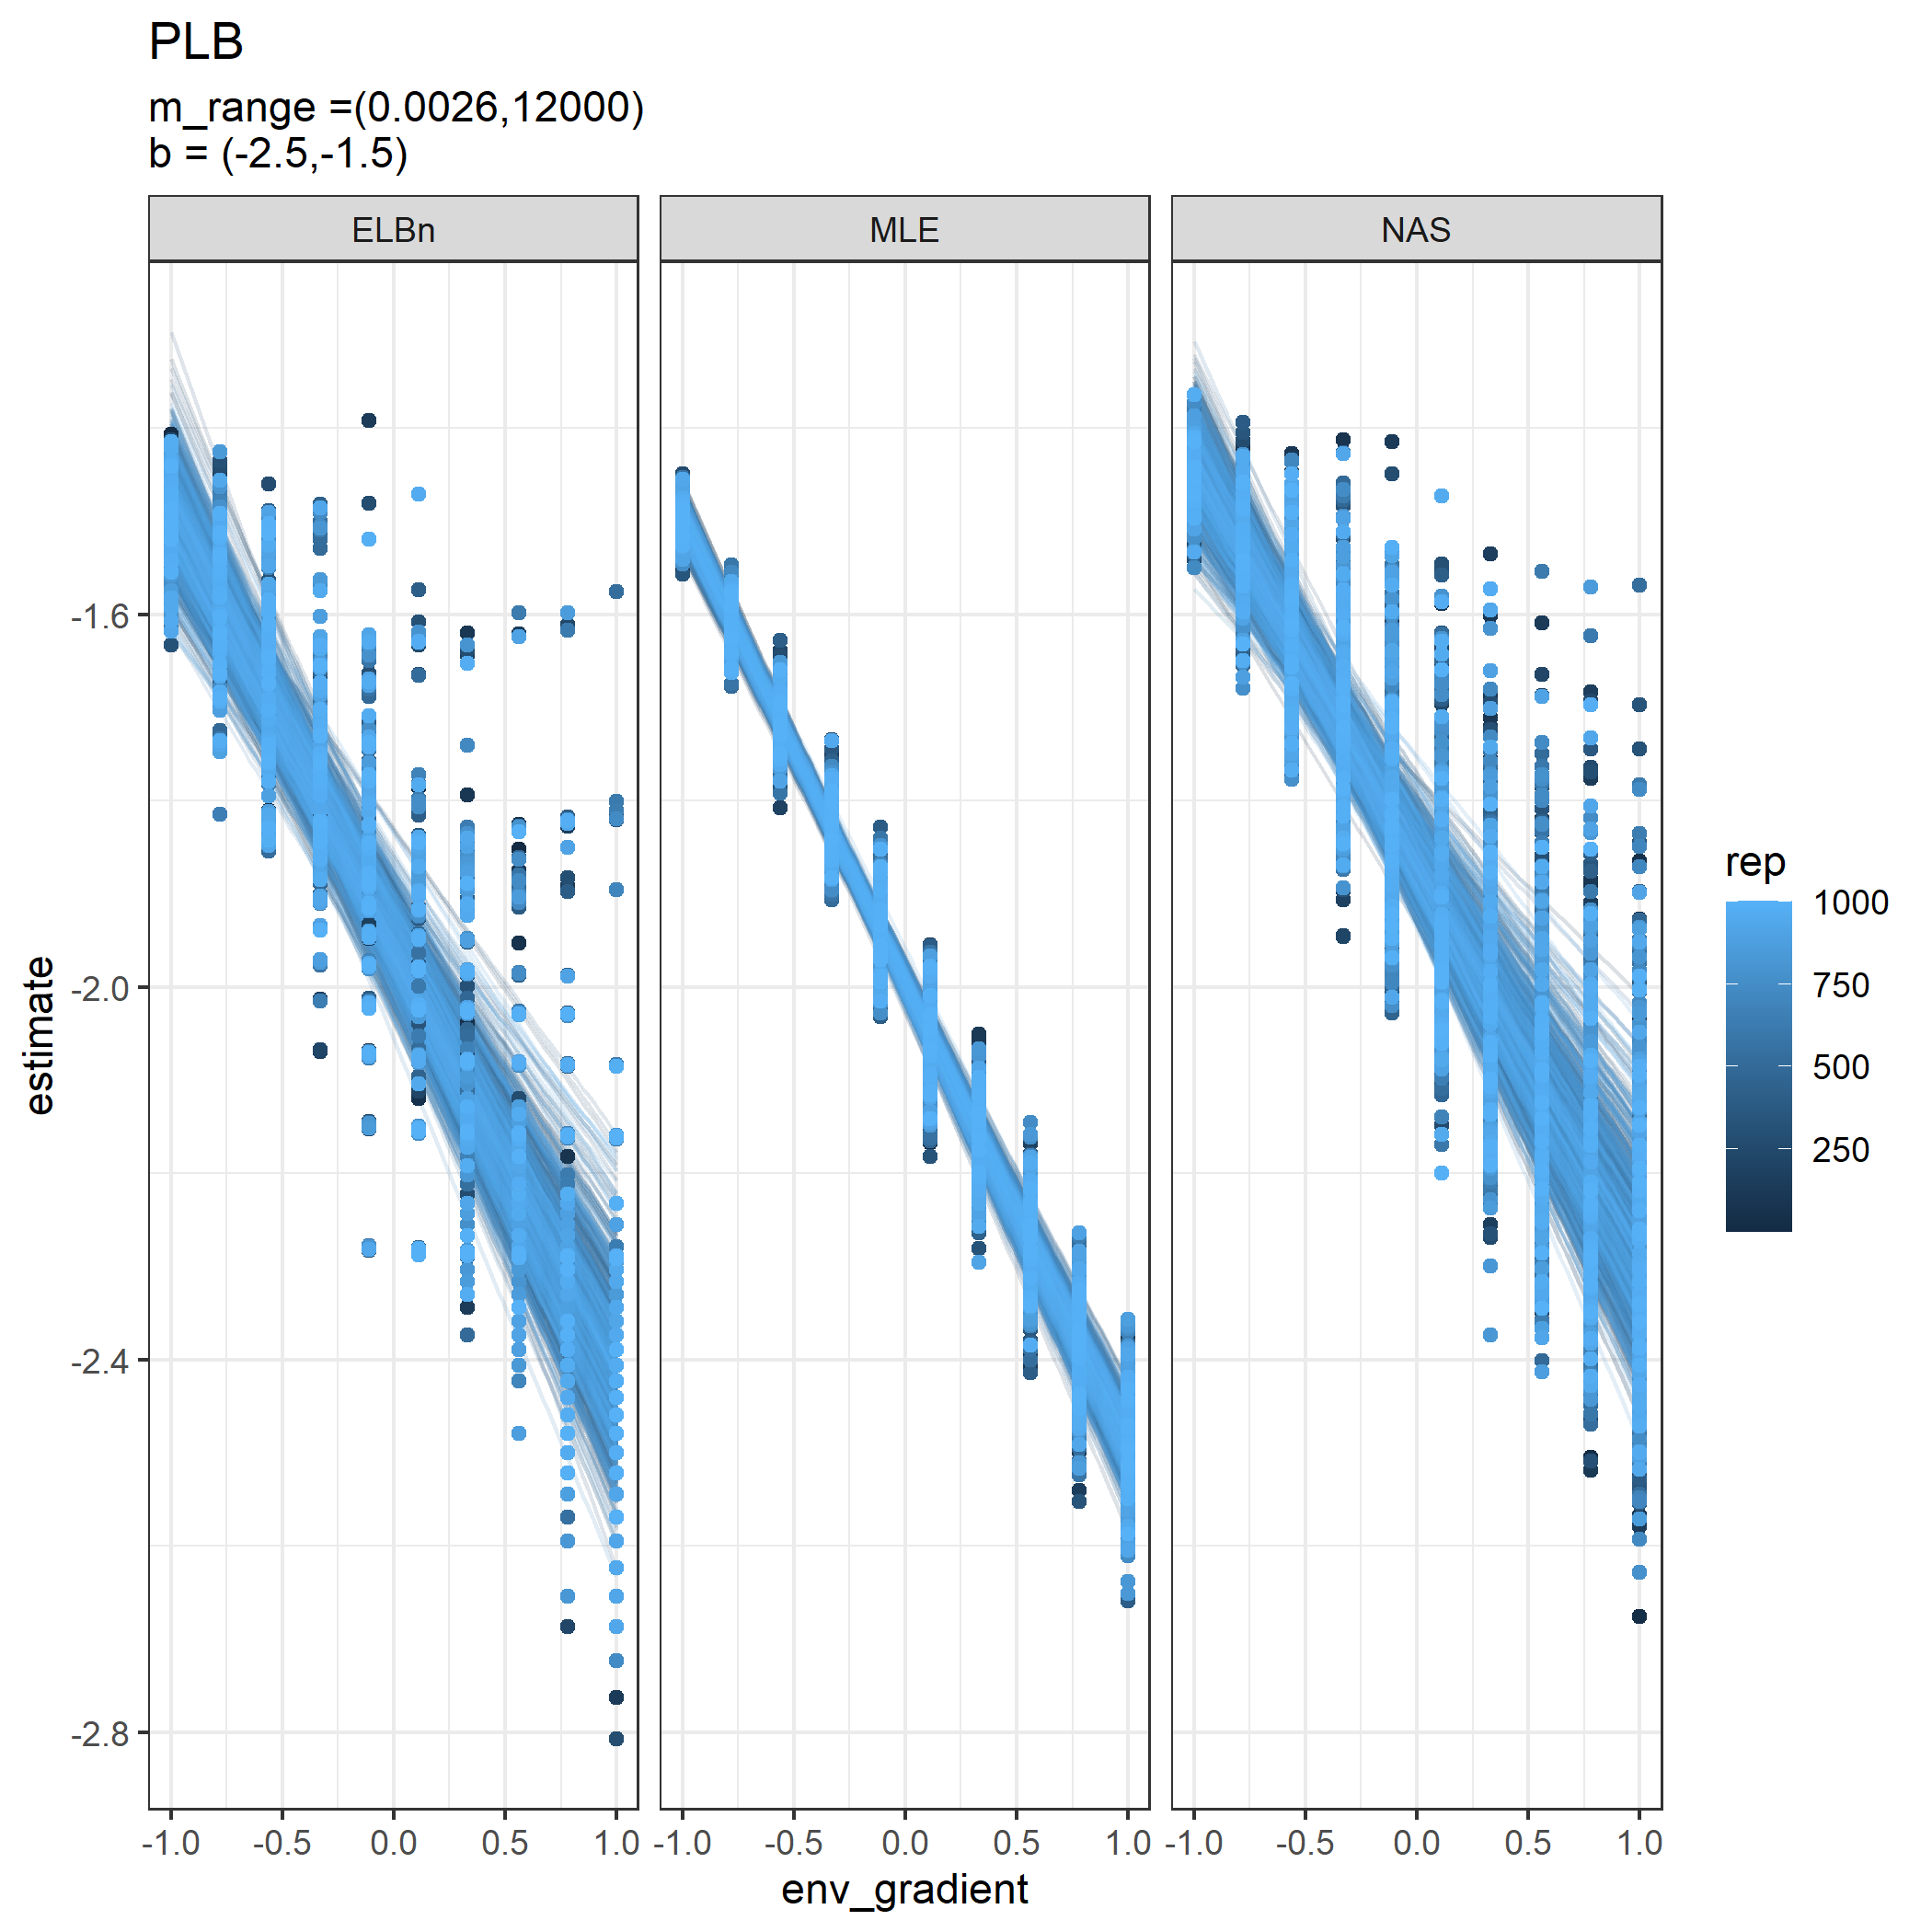
\includegraphics{figures/PLB_10_sites_main.png}
\caption{Individual regressions for ten sites across a hypothetical
gradient with a known relationship of 0.5. All other parameters are the
same as in the main analysis}
\end{figure}

\newpage

\begin{figure}
\centering
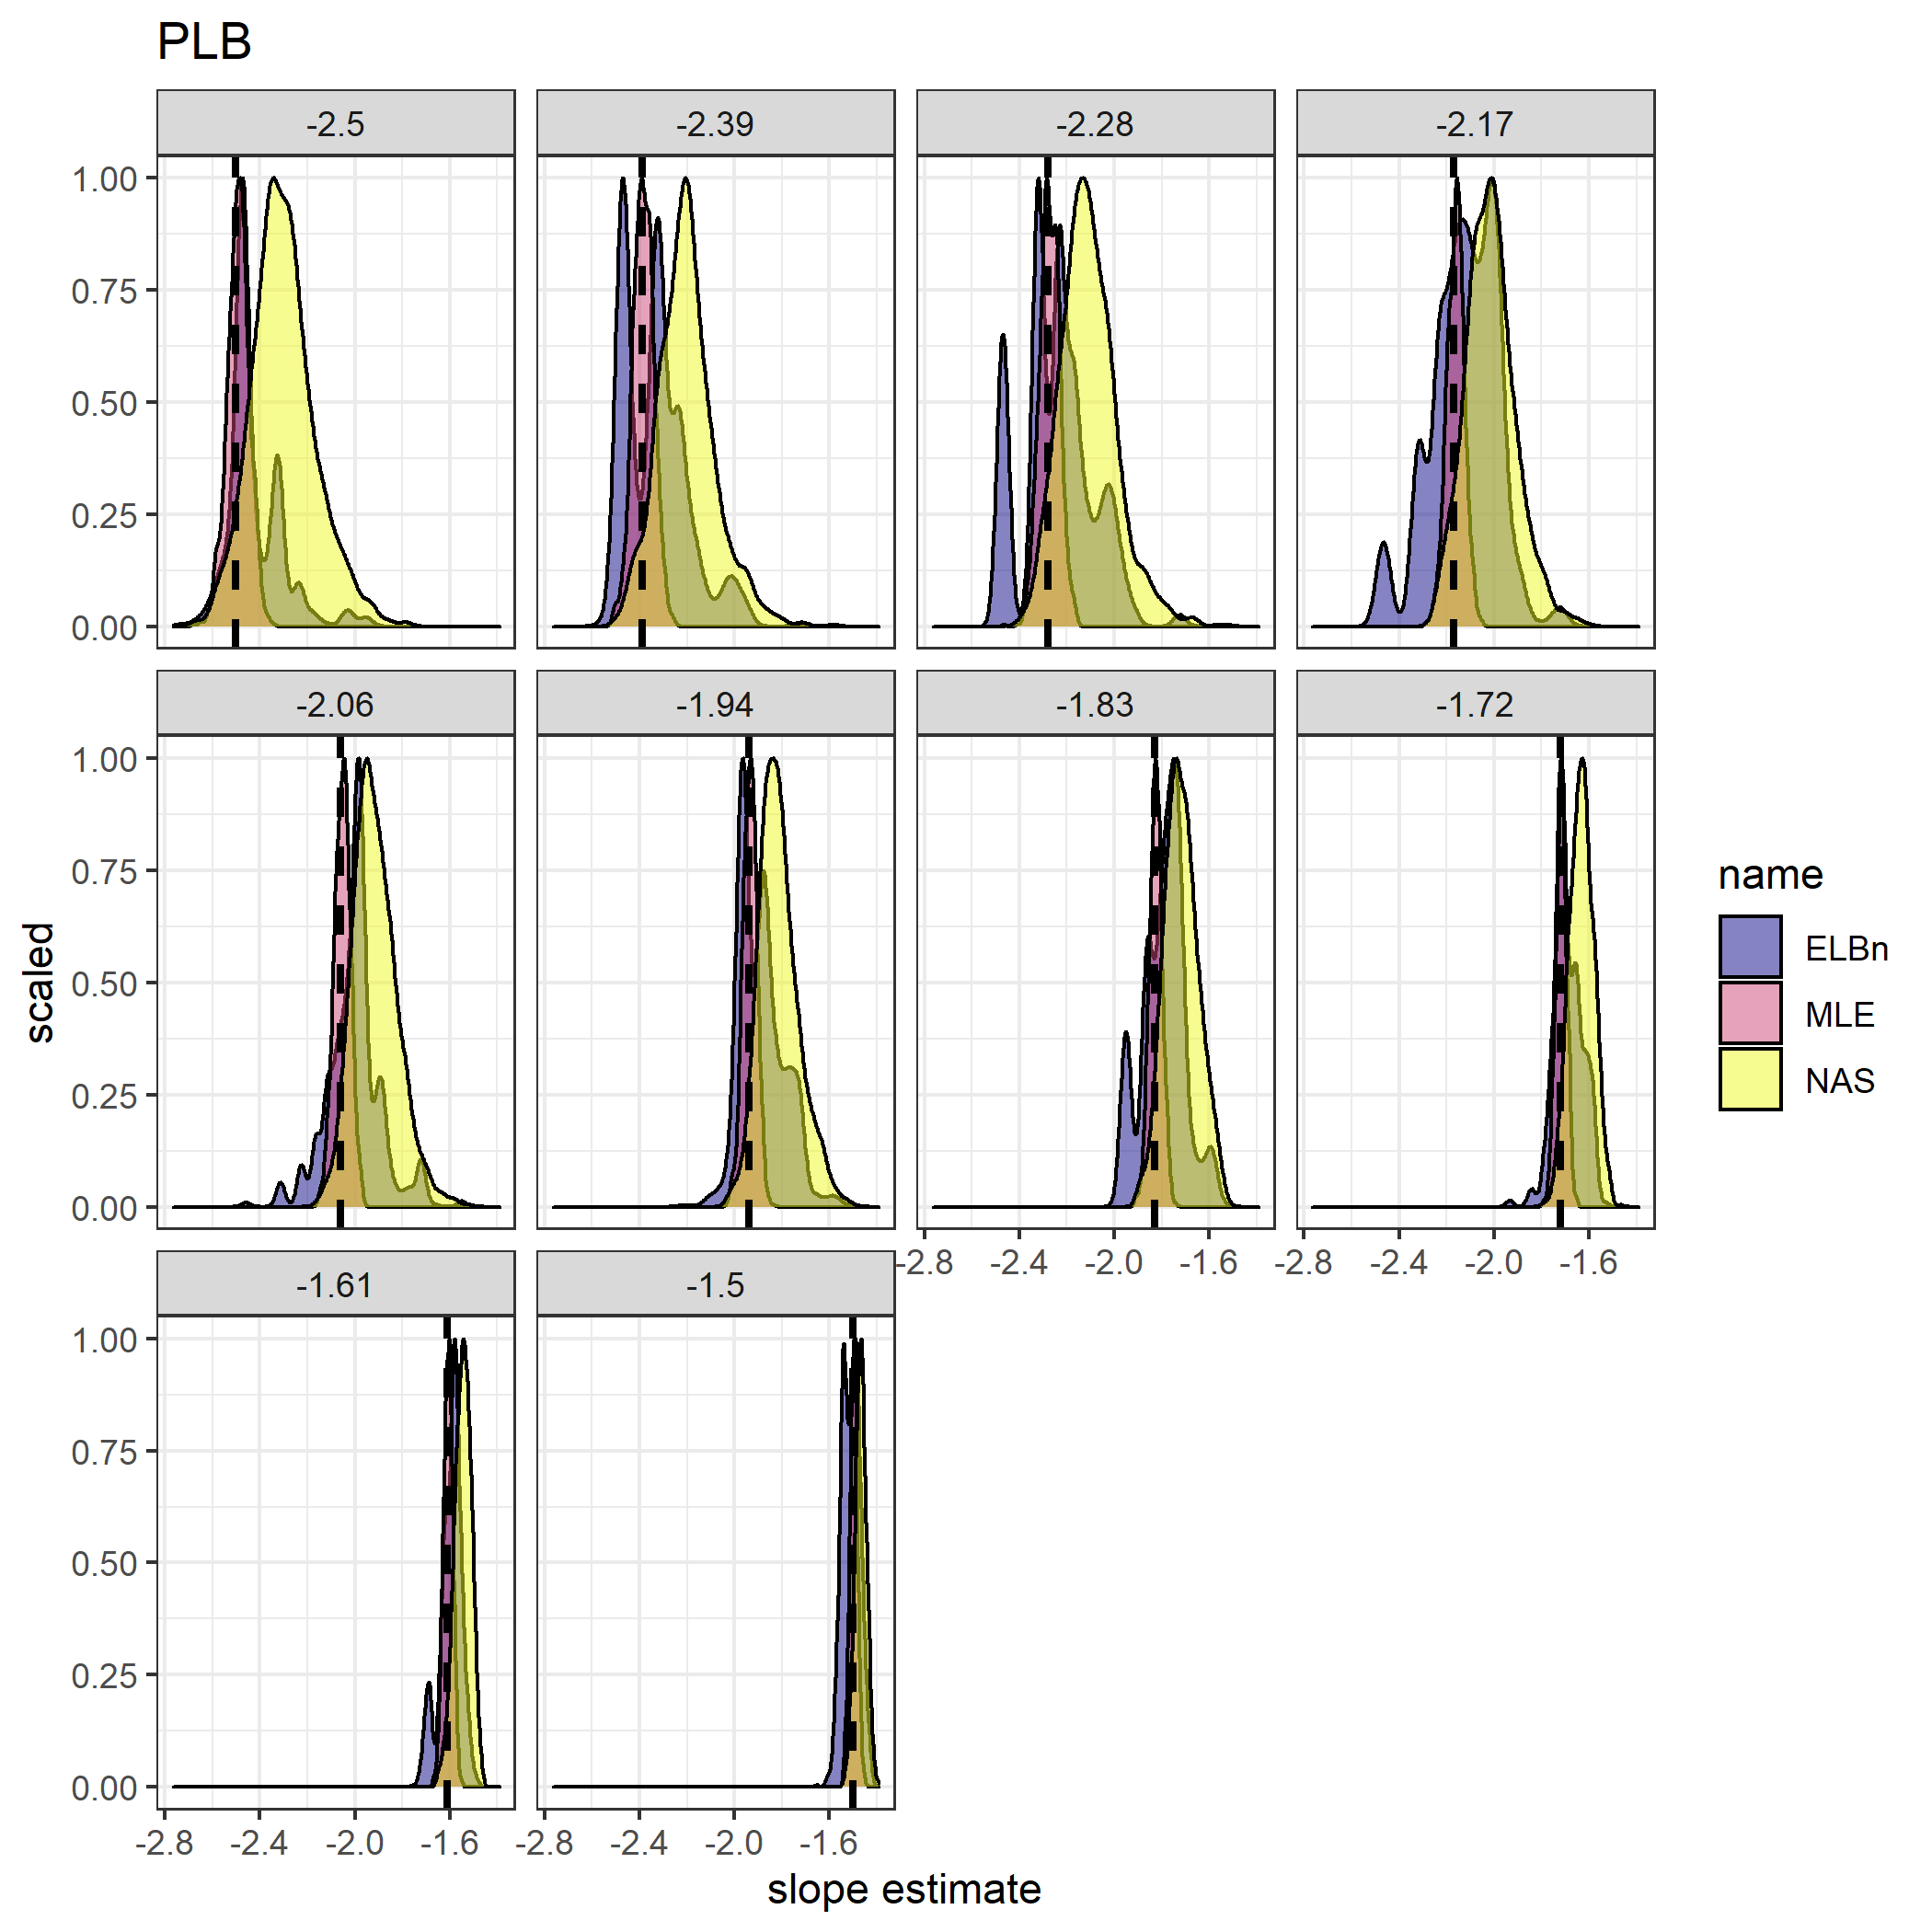
\includegraphics{figures/PLB_10_sites_est_b_density.png}
\caption{Distribution of estimated \(\lambda\) coefficient for ten sites
across a hypothetical gradient with known values. All other parameters
are the same as in the main analysis}
\end{figure}

\newpage

\begin{figure}
\centering
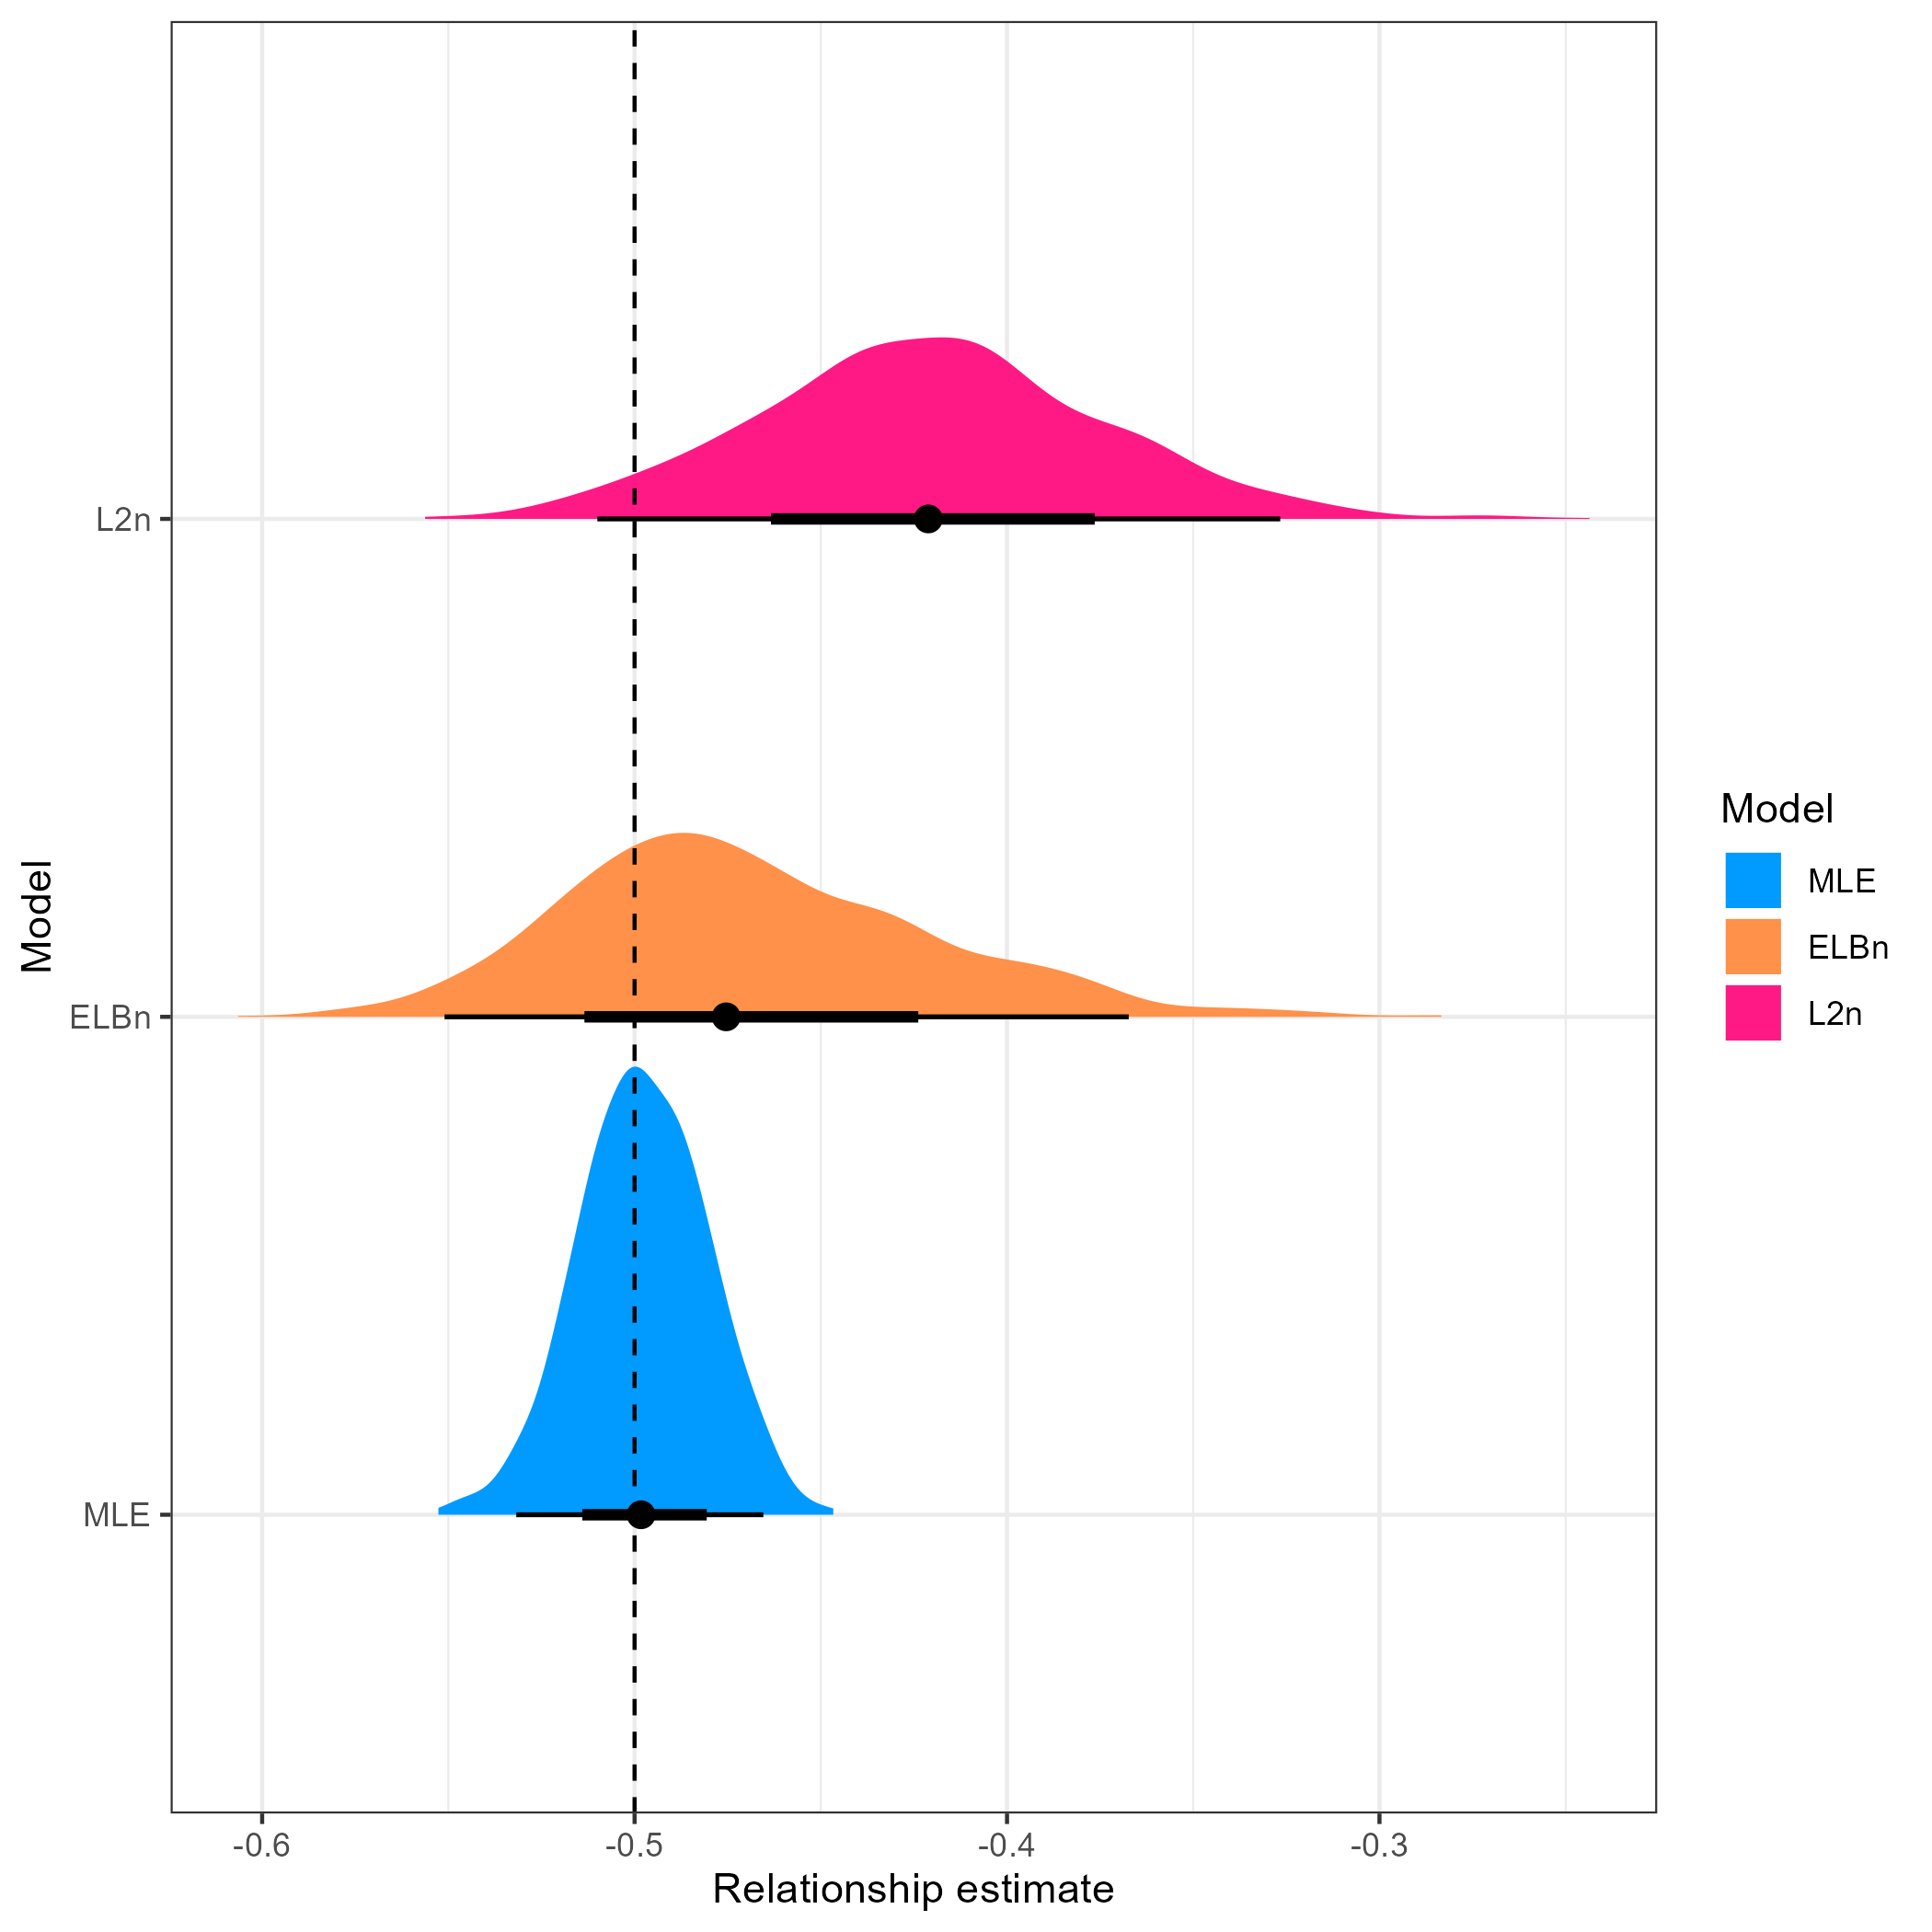
\includegraphics{figures/PLB_10_sites_relationship_density.png}
\caption{Distribution of estimated relationship (\(\beta_1\))
coefficient's for ten sites across a hypothetical gradient with known
value of 0.5. All other parameters are the same as in the main analysis}
\end{figure}

\newpage

\hypertarget{three-sites}{%
\subsubsection{Three sites}\label{three-sites}}

\begin{figure}
\centering
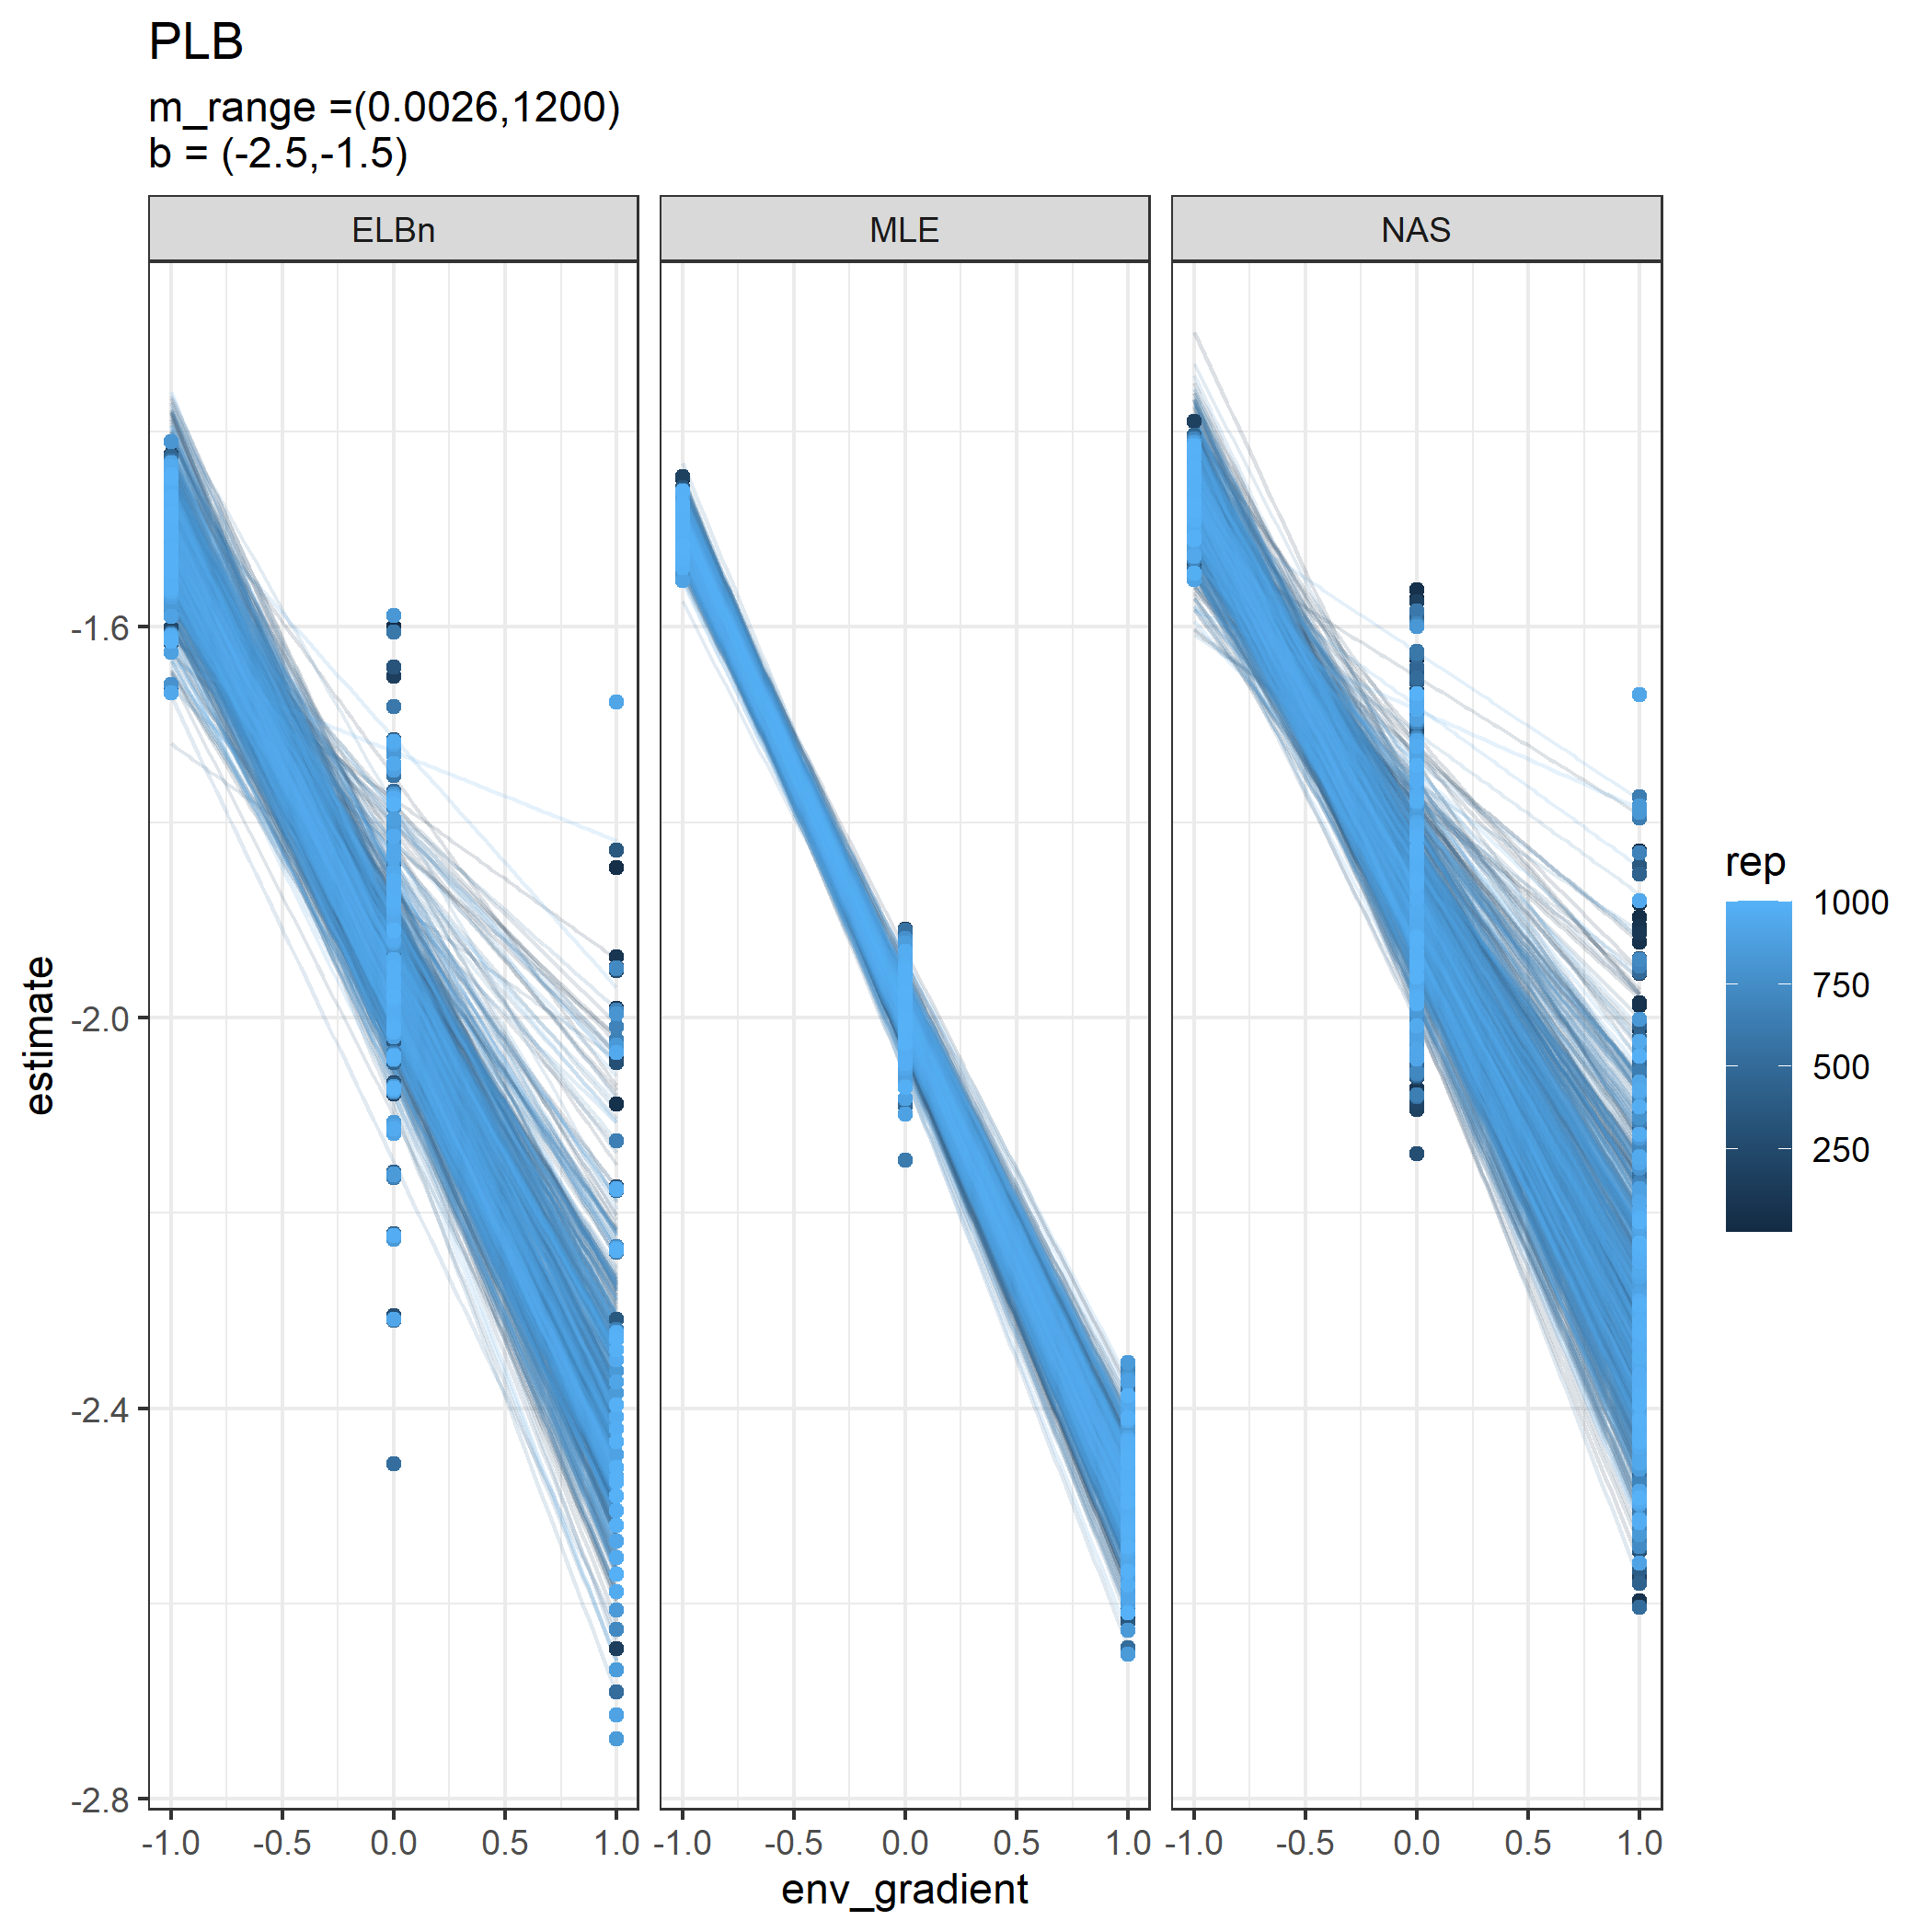
\includegraphics{figures/PLB_3_sites_main.png}
\caption{Individual regressions for three sites across a hypothetical
gradient with a known relationship of 0.5. All other parameters are the
same as in the main analysis.}
\end{figure}

\newpage

\begin{figure}
\centering
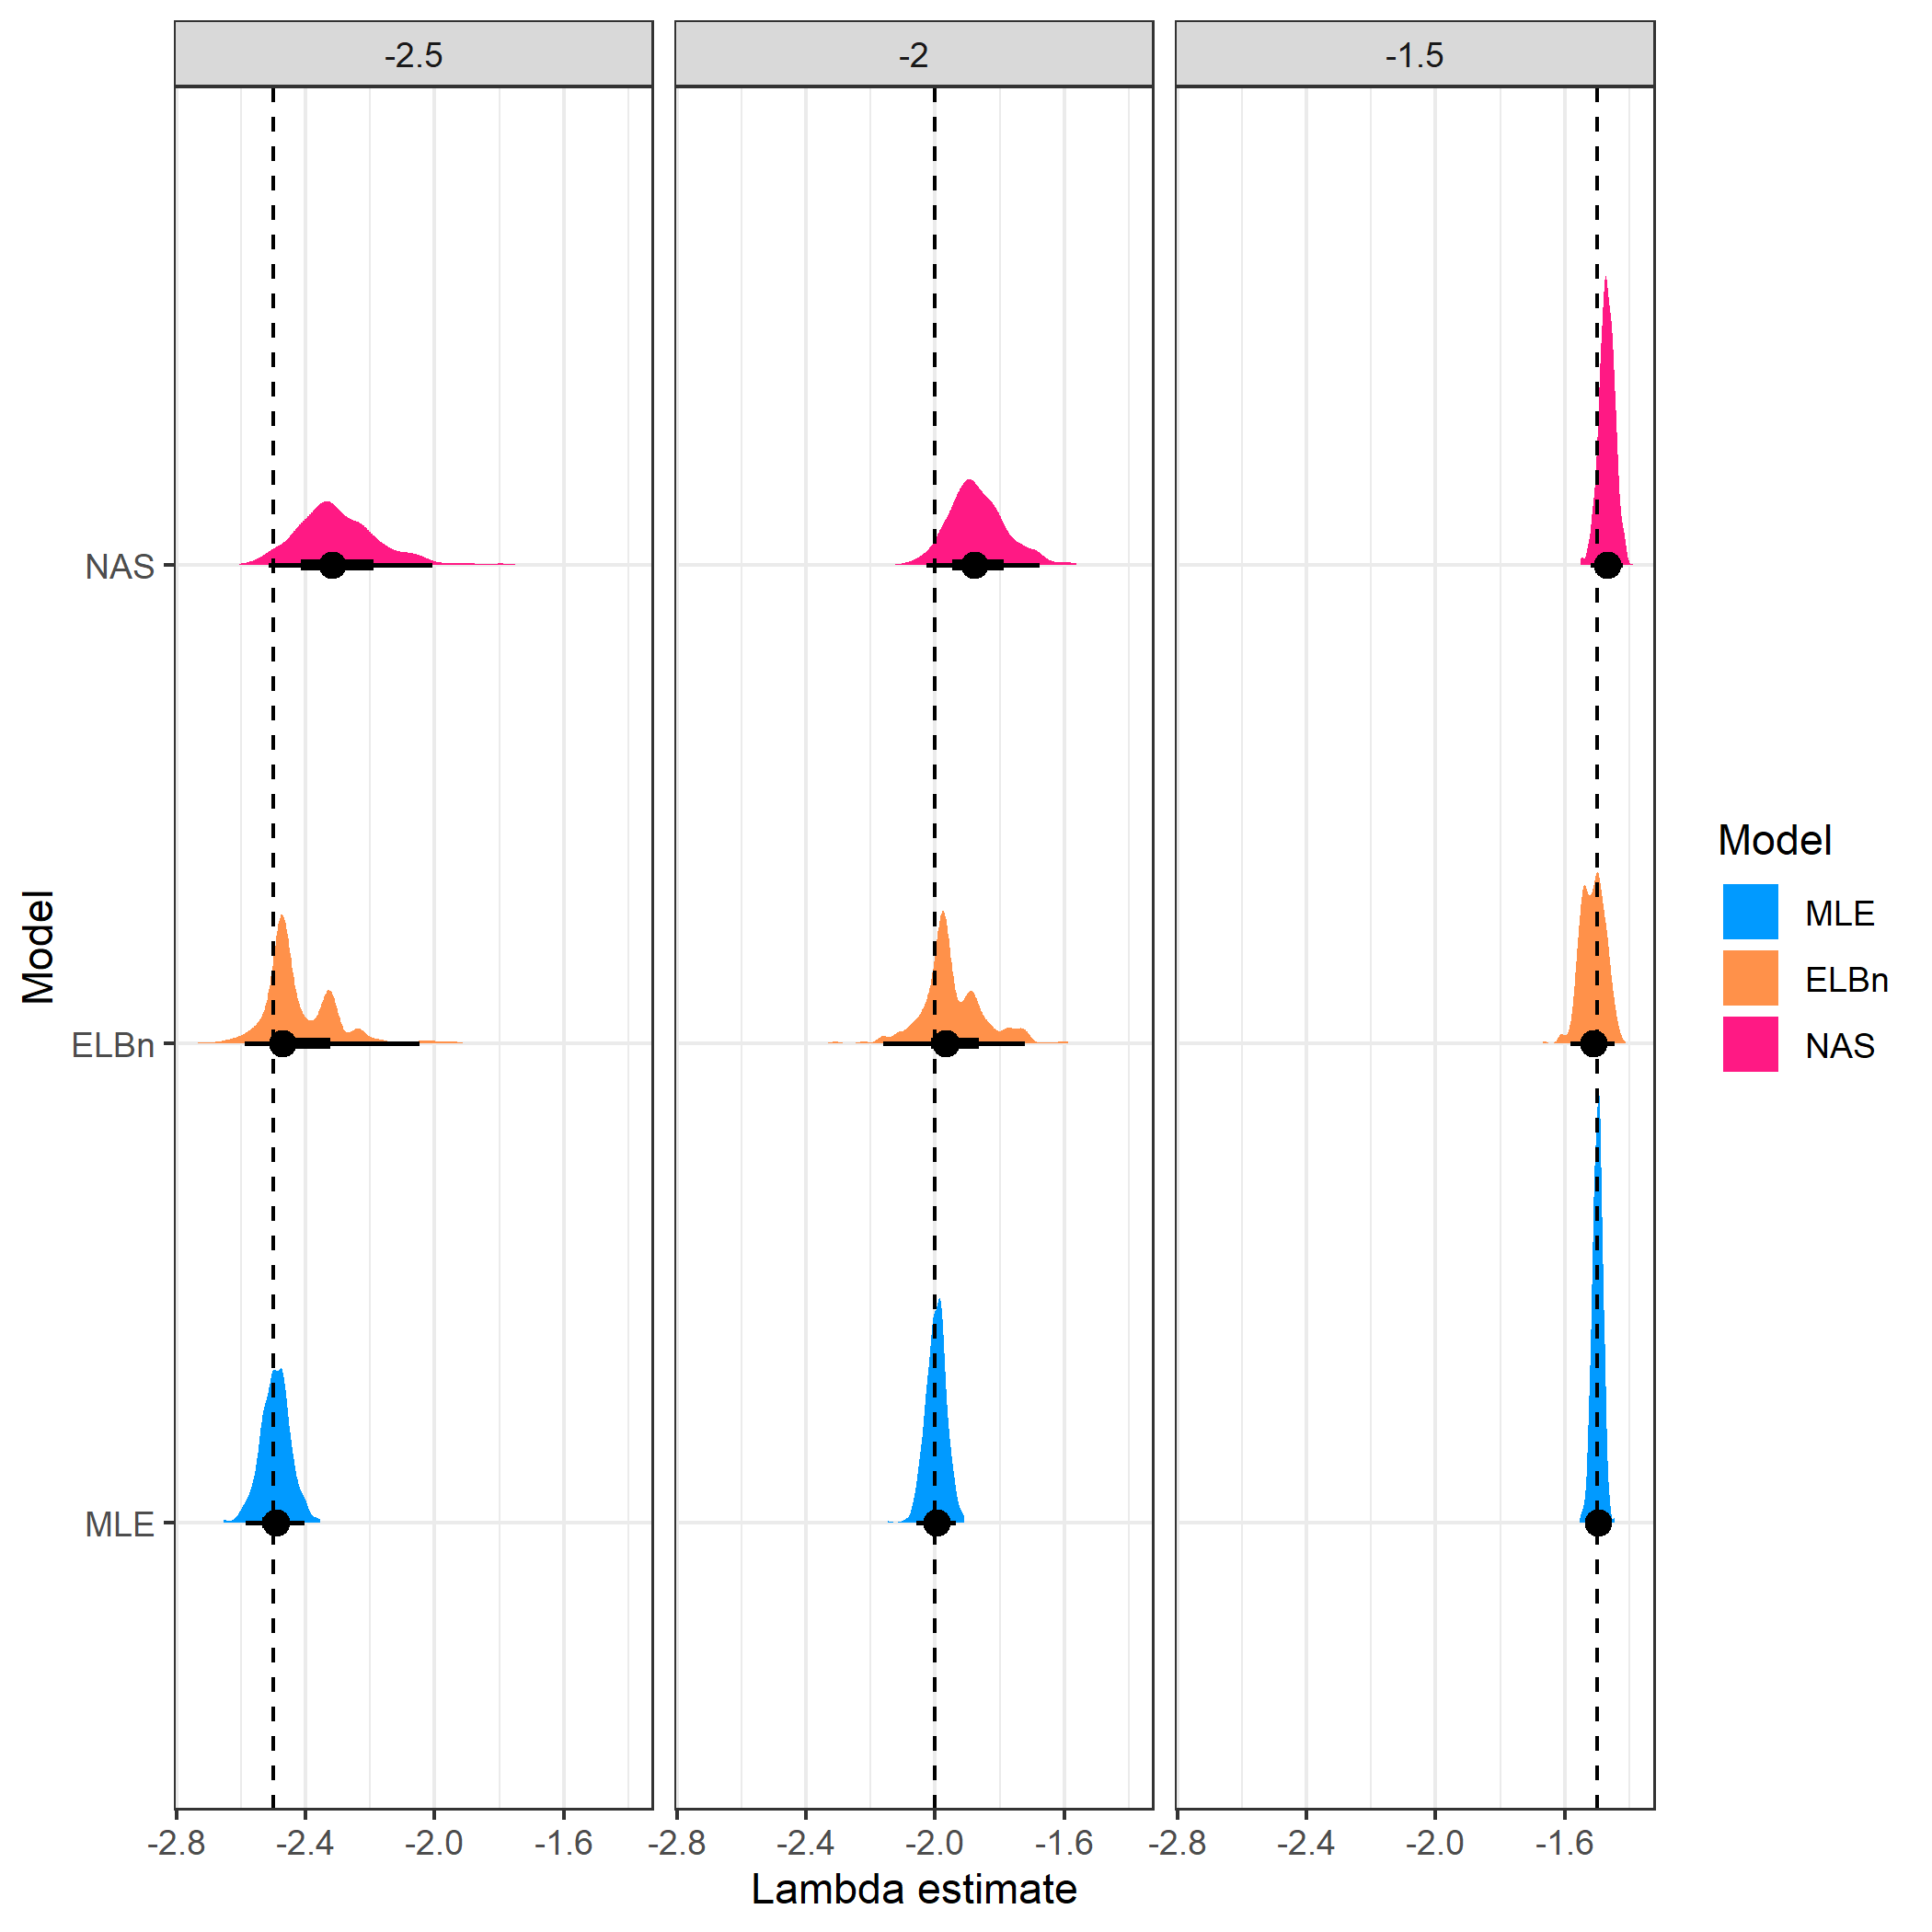
\includegraphics{figures/PLB_3_sites_est_b_density.png}
\caption{Distribution of estimated \(\lambda\) coefficient for three
sites across a hypothetical gradient with known values. All other
parameters are the same as in the main analysis.}
\end{figure}

\newpage

\begin{figure}
\centering
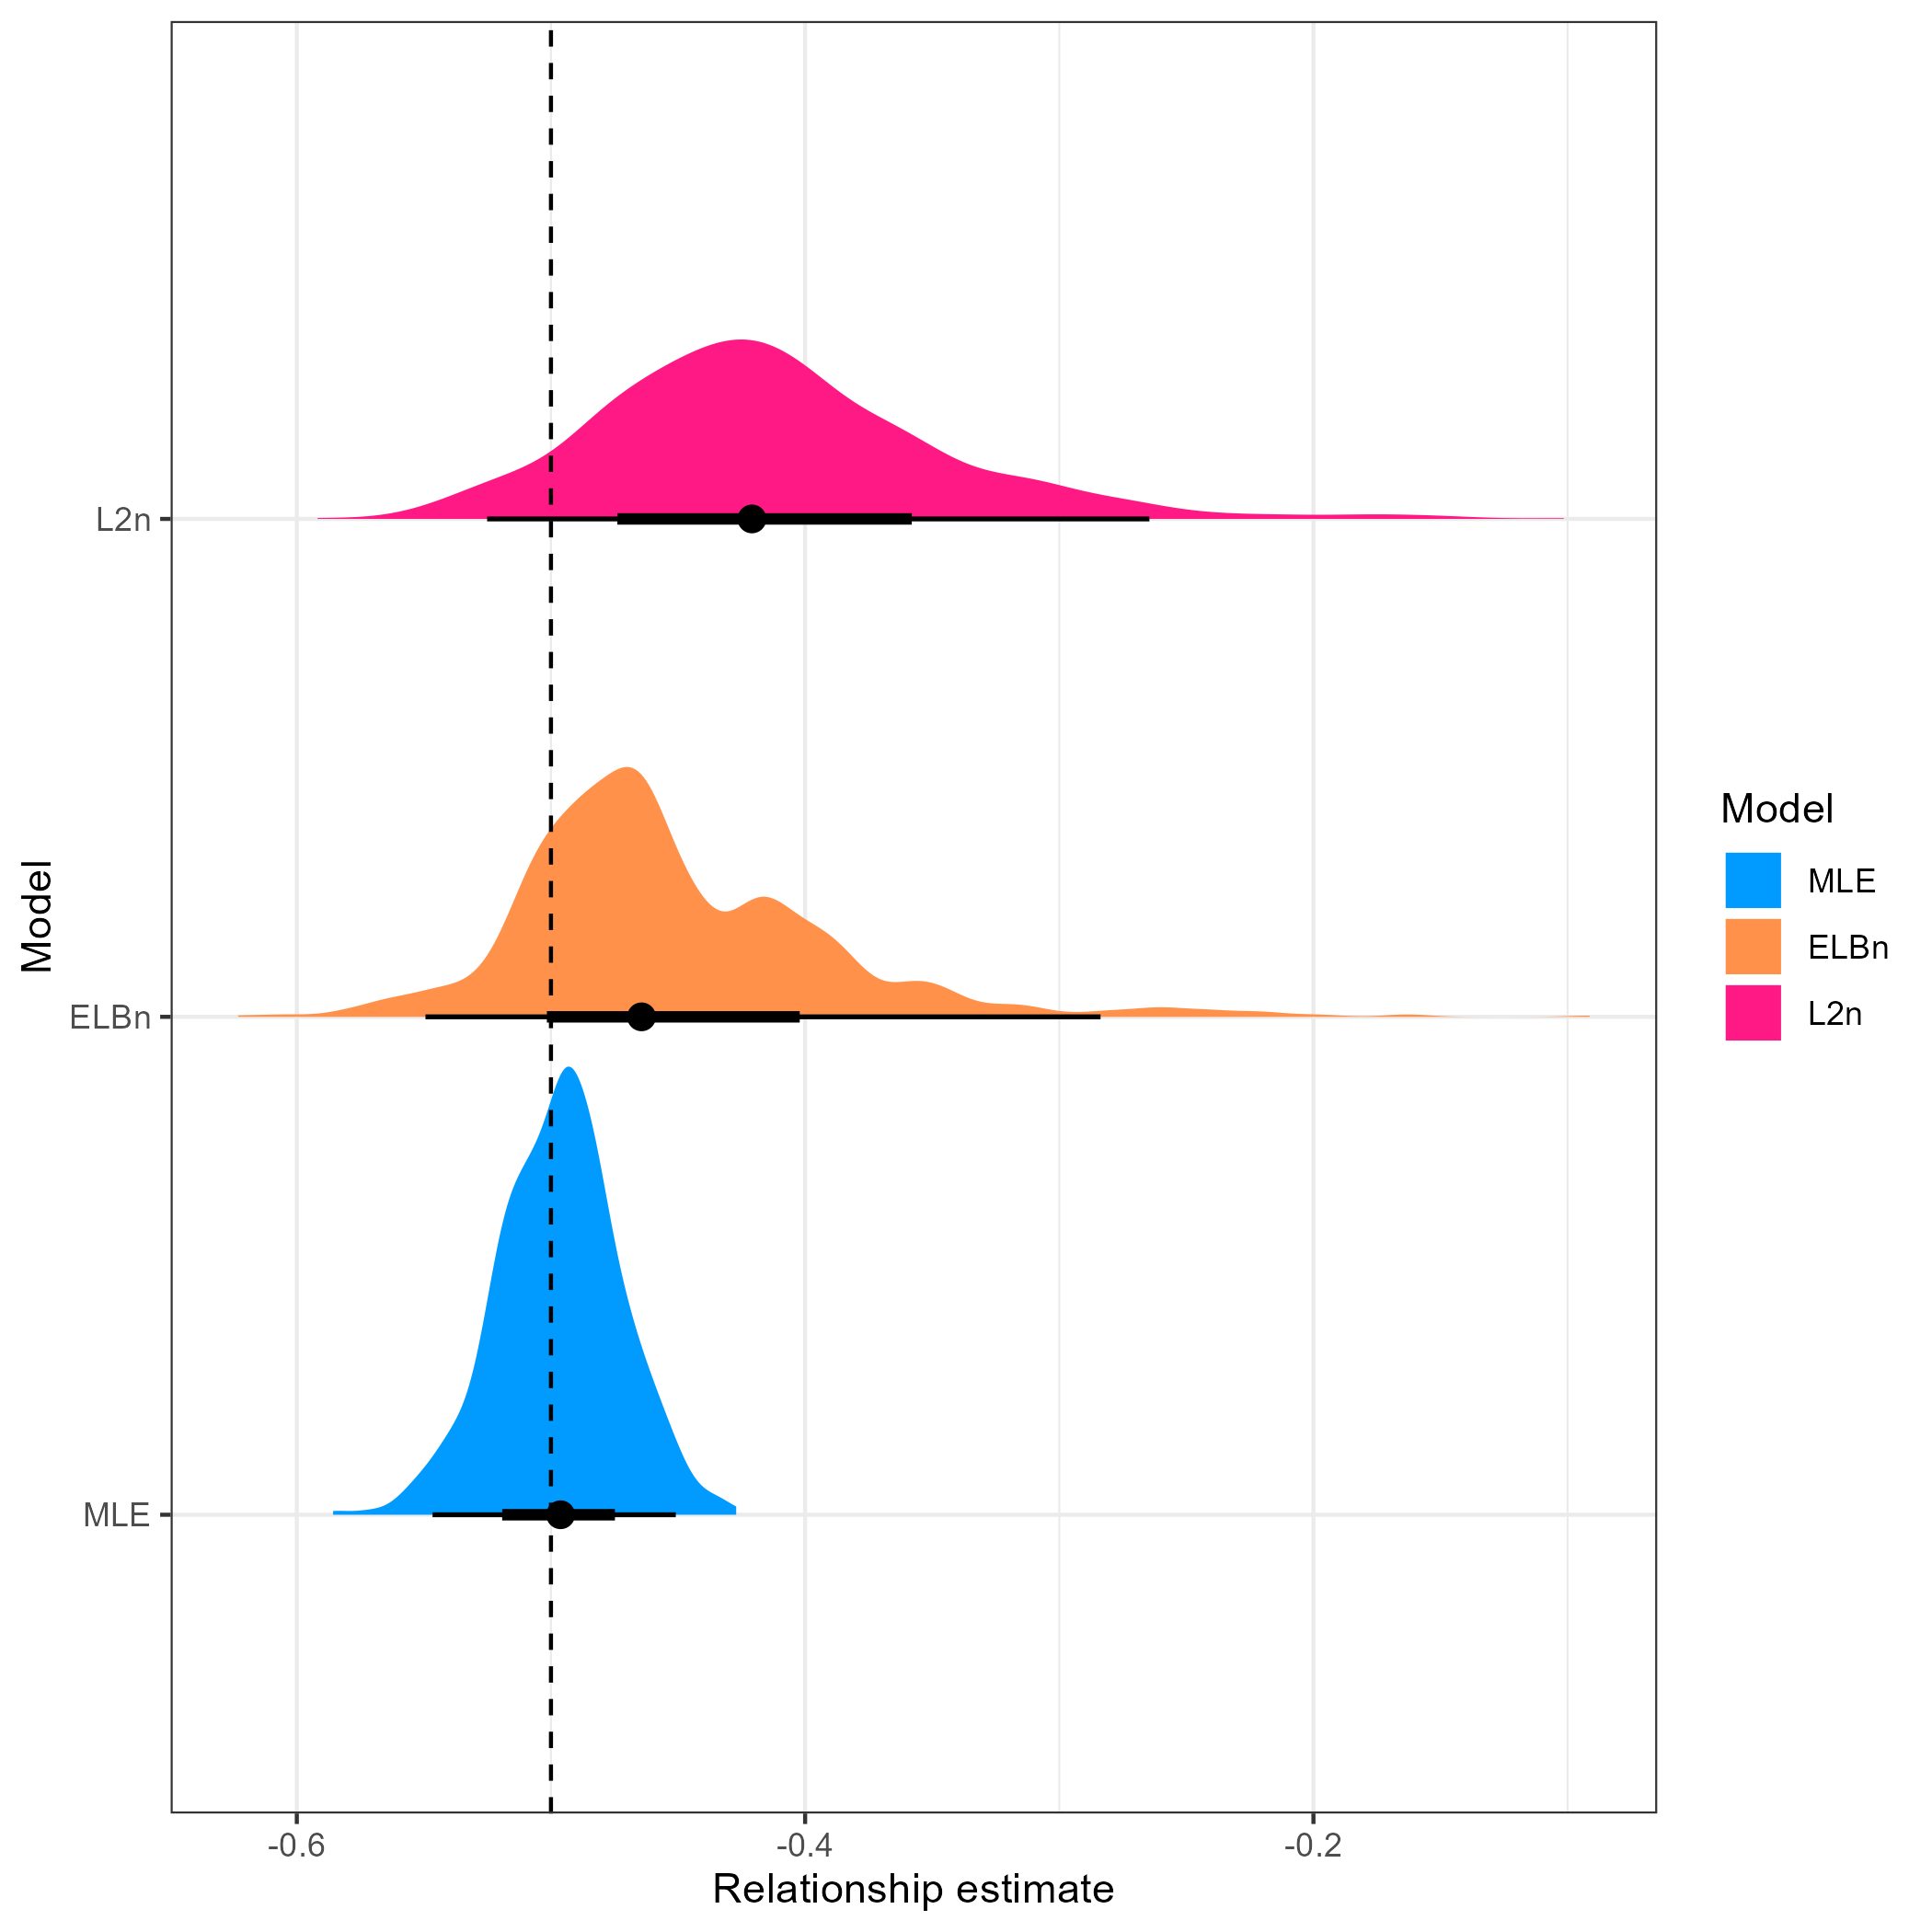
\includegraphics{figures/PLB_3_sites_relationship_density.png}
\caption{Distribution of estimated relationship (\(\beta_1\))
coefficient's for three sites across a hypothetical gradient with known
value of 0.5. All other parameters are the same as in the main analysis}
\end{figure}

\newpage

\hypertarget{large-environmental-gradient}{%
\subsection{Large environmental
gradient}\label{large-environmental-gradient}}

\begin{figure}
\centering
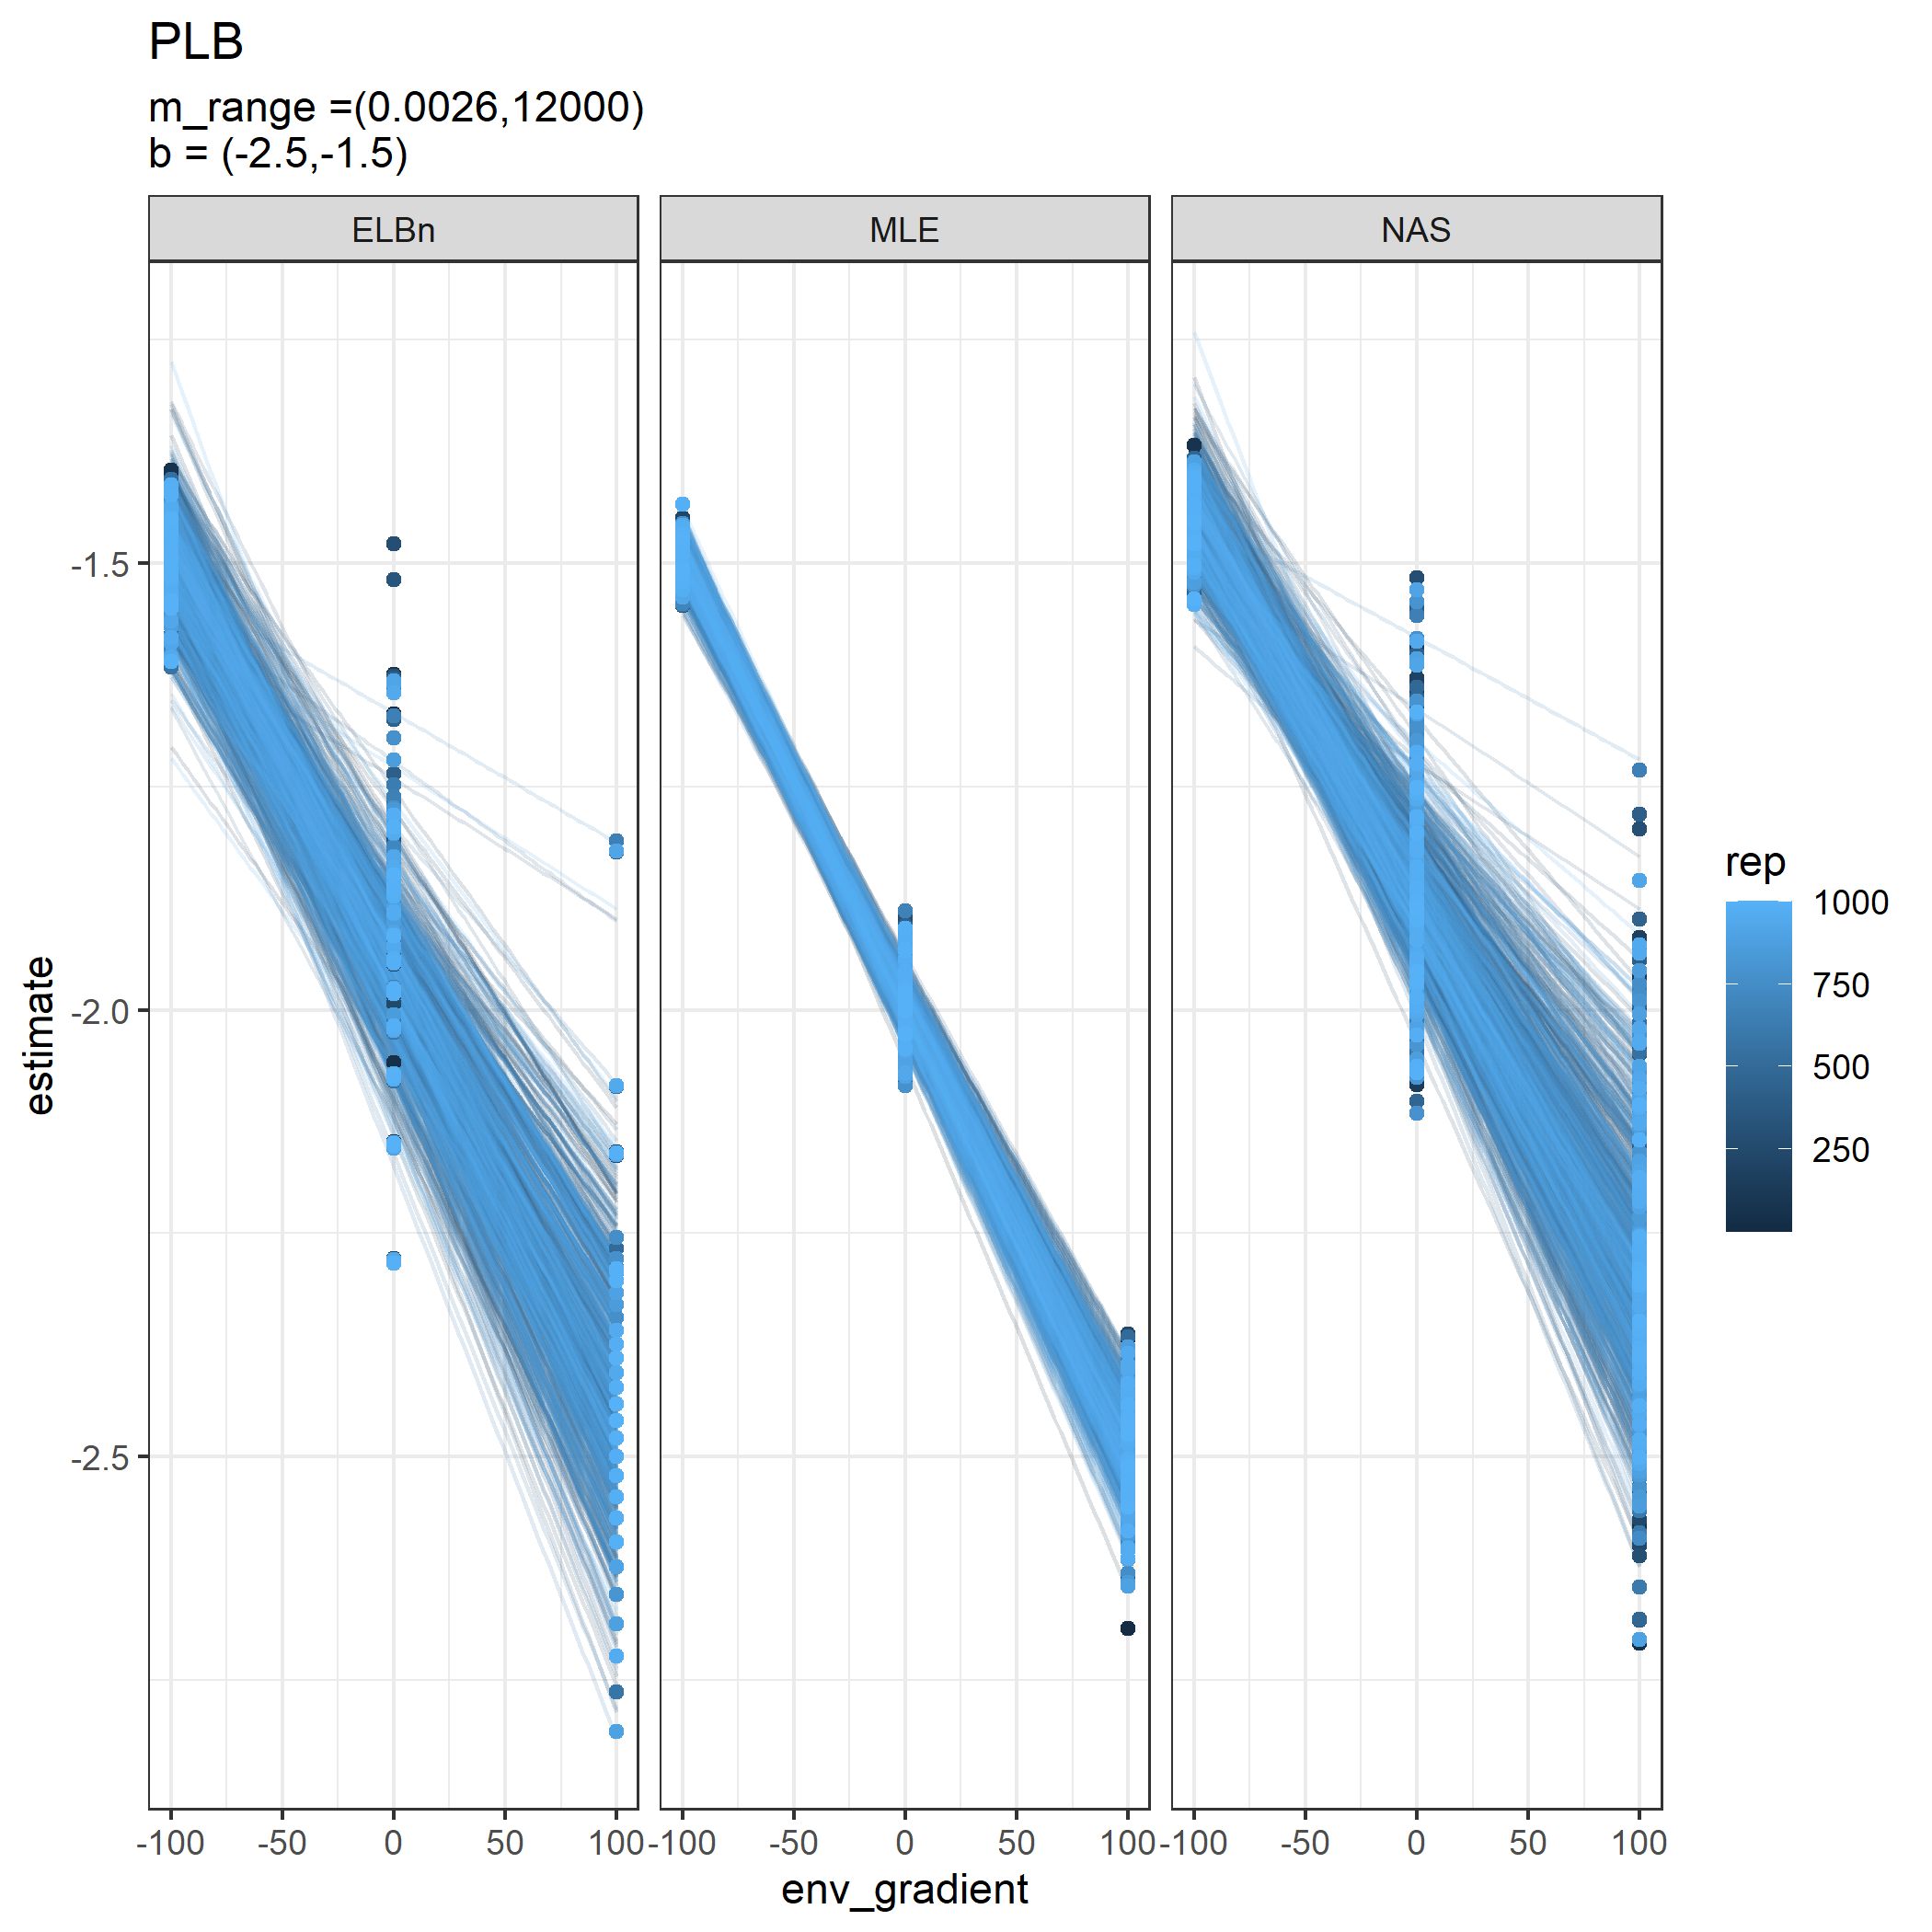
\includegraphics{figures/PLB_large_x_main.png}
\caption{Individual regressions for five sites across a hypothetical
gradient with a known relationship of 0.5. Range of environmental values
(\emph{x}-axis) increased to be -1000, to 1000.}
\end{figure}

\newpage

\begin{figure}
\centering
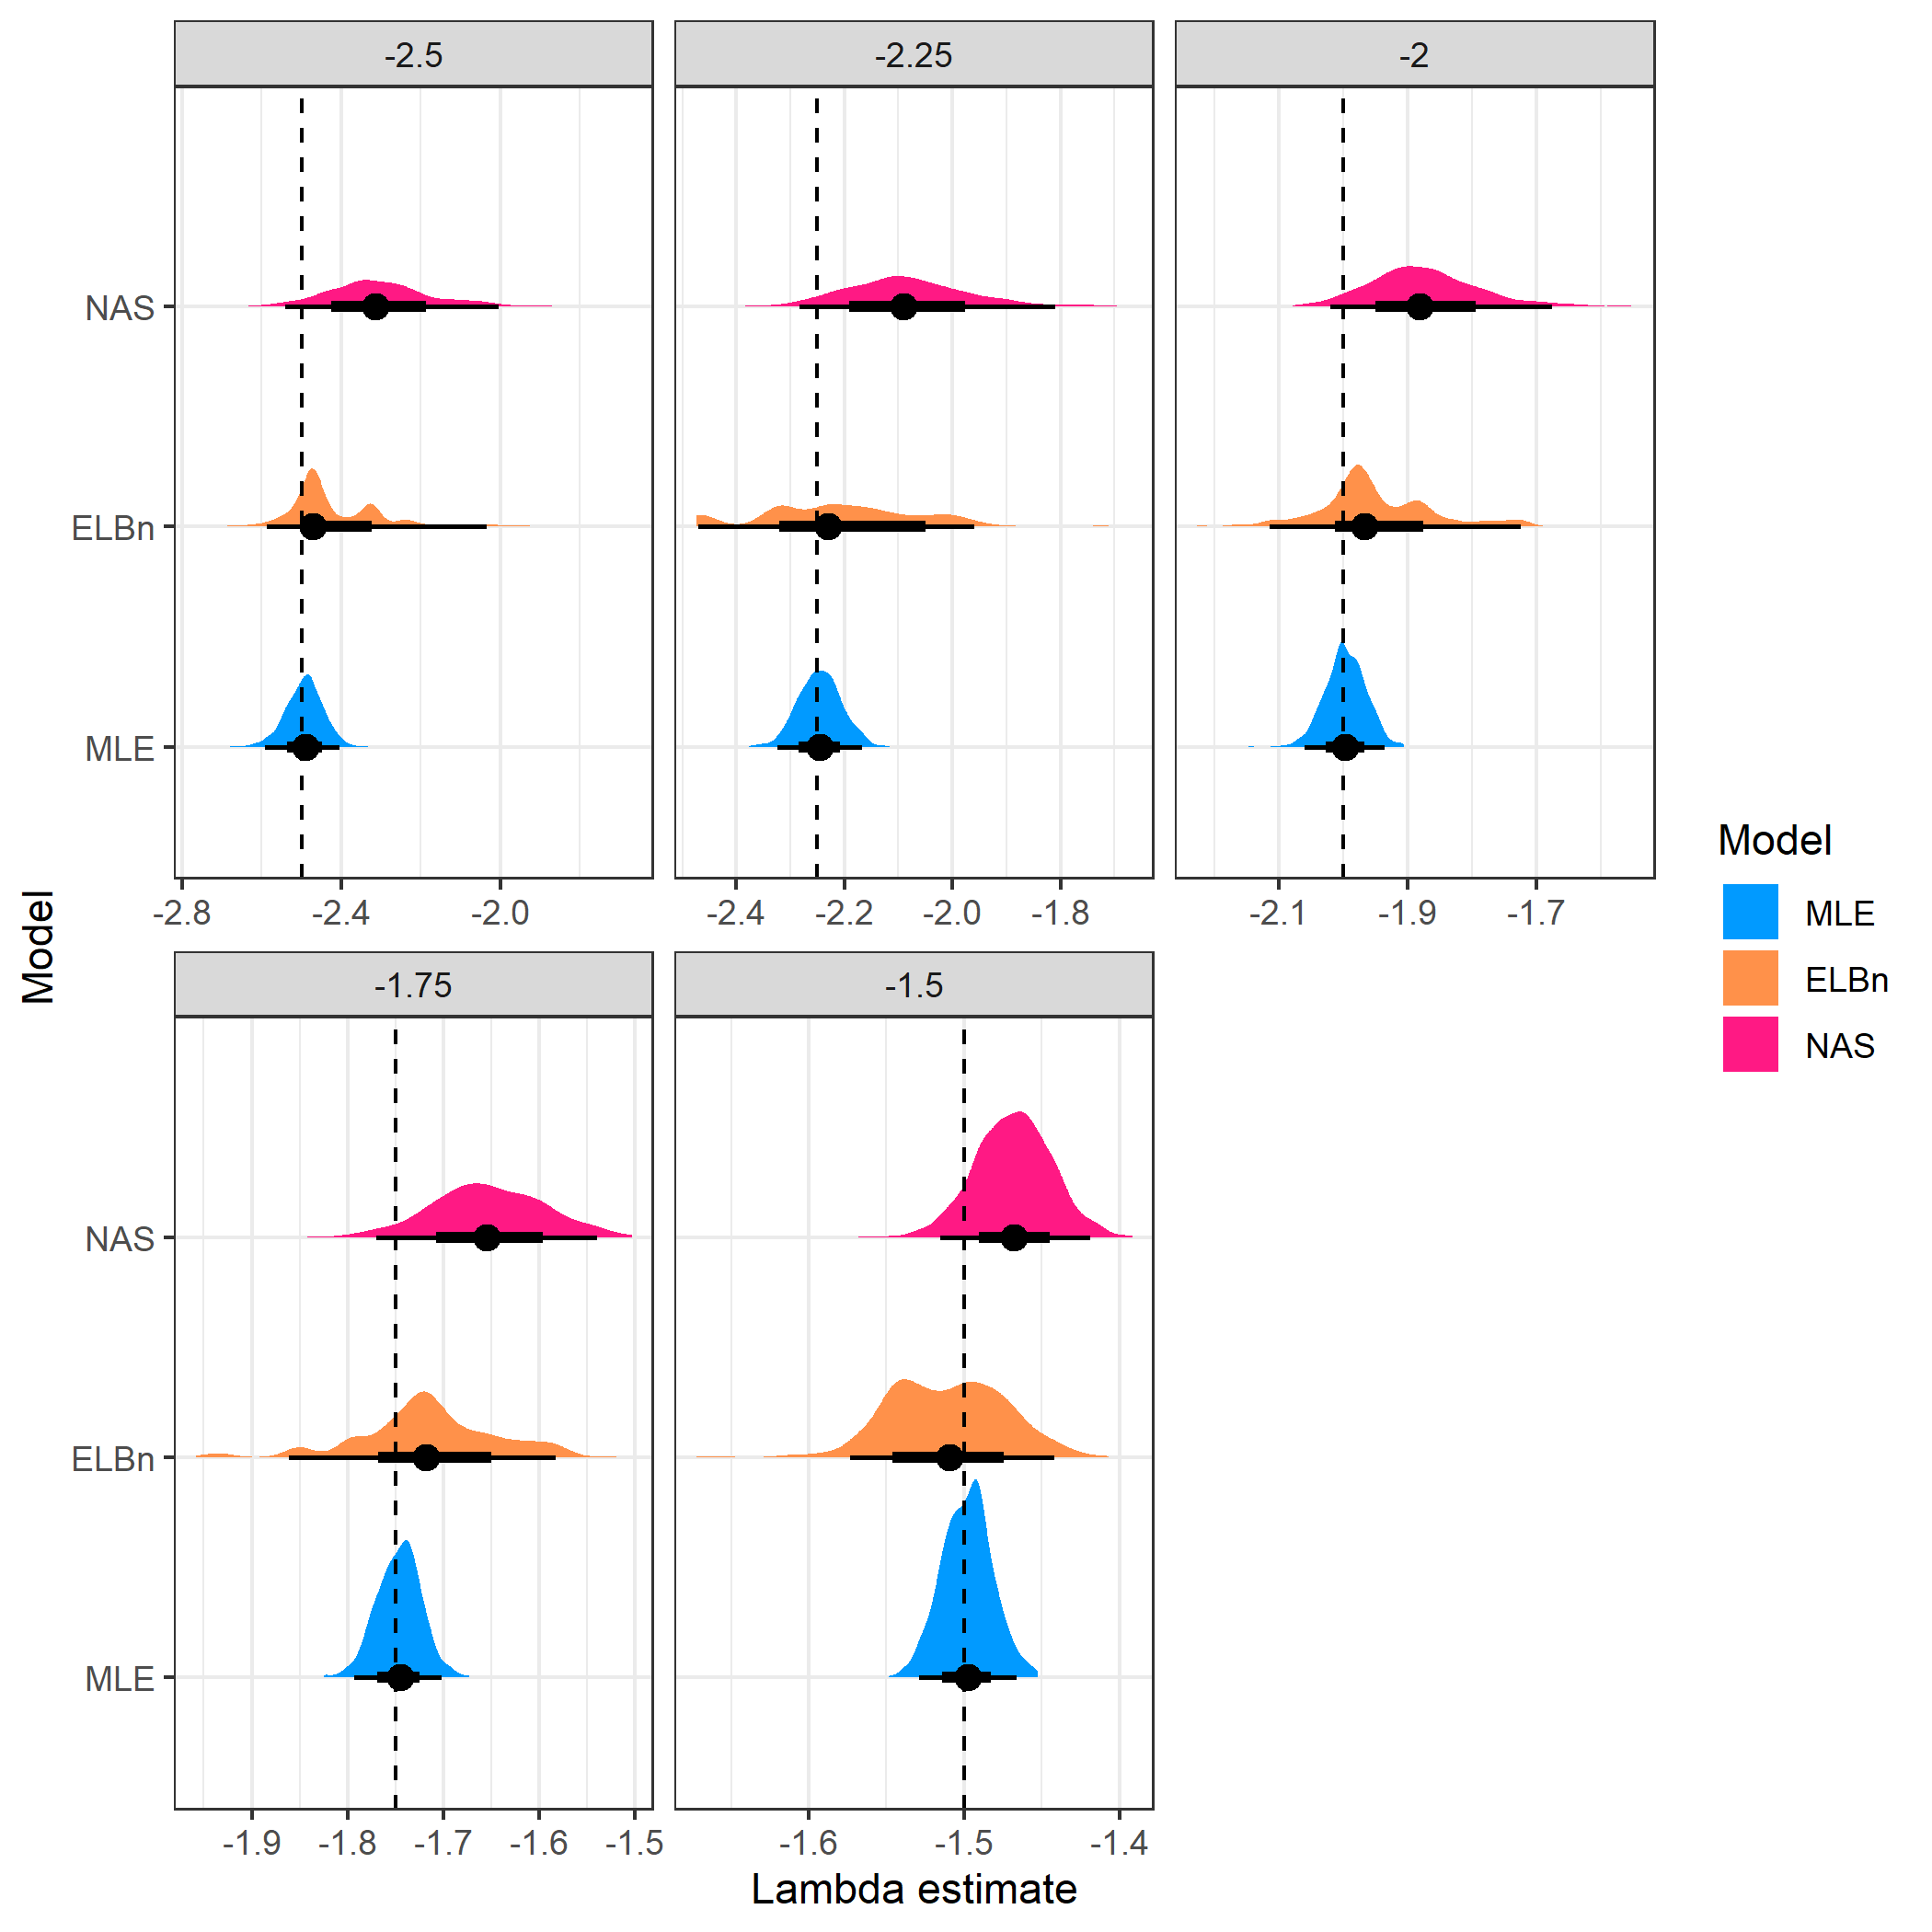
\includegraphics{figures/PLB_large_x_est_b_density.png}
\caption{Distribution of estimated \(\lambda\) coefficient for five
sites across a hypothetical gradient with known values. Range of
environmental values (\emph{x}-axis) increased to be -1000, to 1000.}
\end{figure}

\newpage

\begin{figure}
\centering
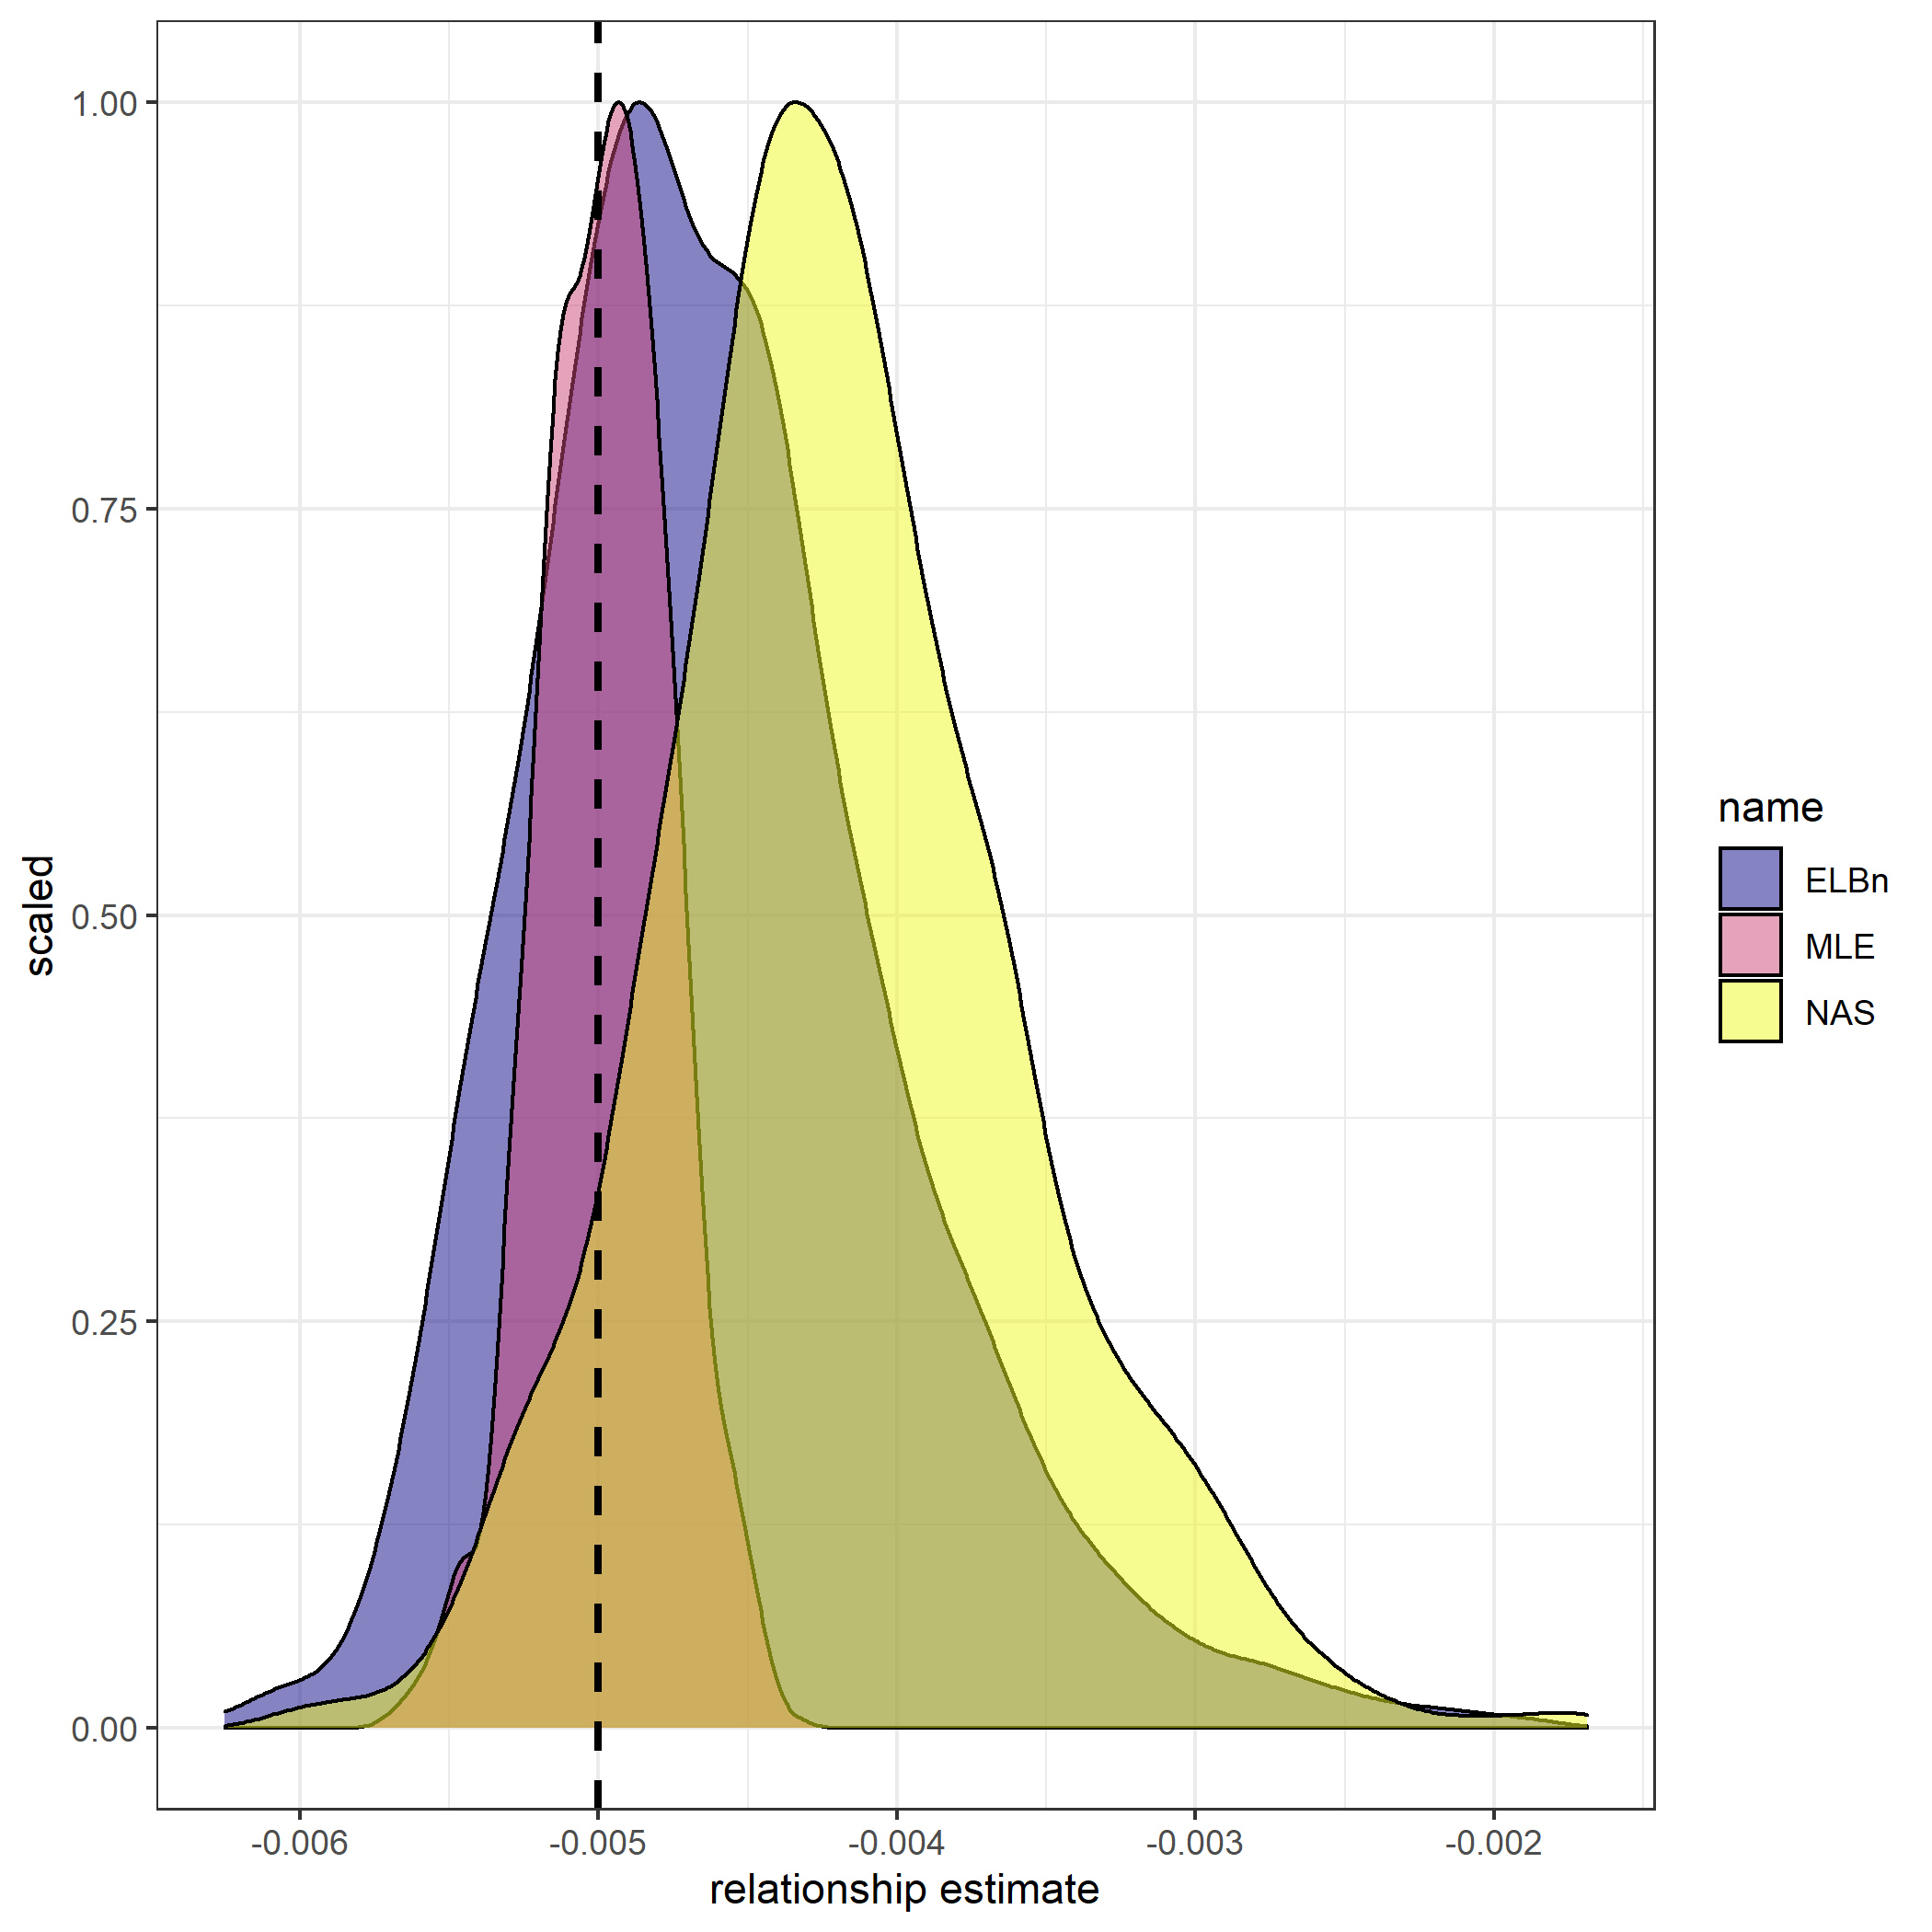
\includegraphics{figures/PLB_large_x_relationship_density.png}
\caption{Distribution of estimated relationship (\(\beta_1\))
coefficient's for five sites across a hypothetical gradient with known
value of 0.5. Range of environmental values (\emph{x}-axis) increased to
be -1000, to 1000.}
\end{figure}

\newpage

\hypertarget{range-of-body-sizes-m}{%
\subsection{\texorpdfstring{Range of body sizes,
\(M\)}{Range of body sizes, M}}\label{range-of-body-sizes-m}}

\begin{figure}
\centering
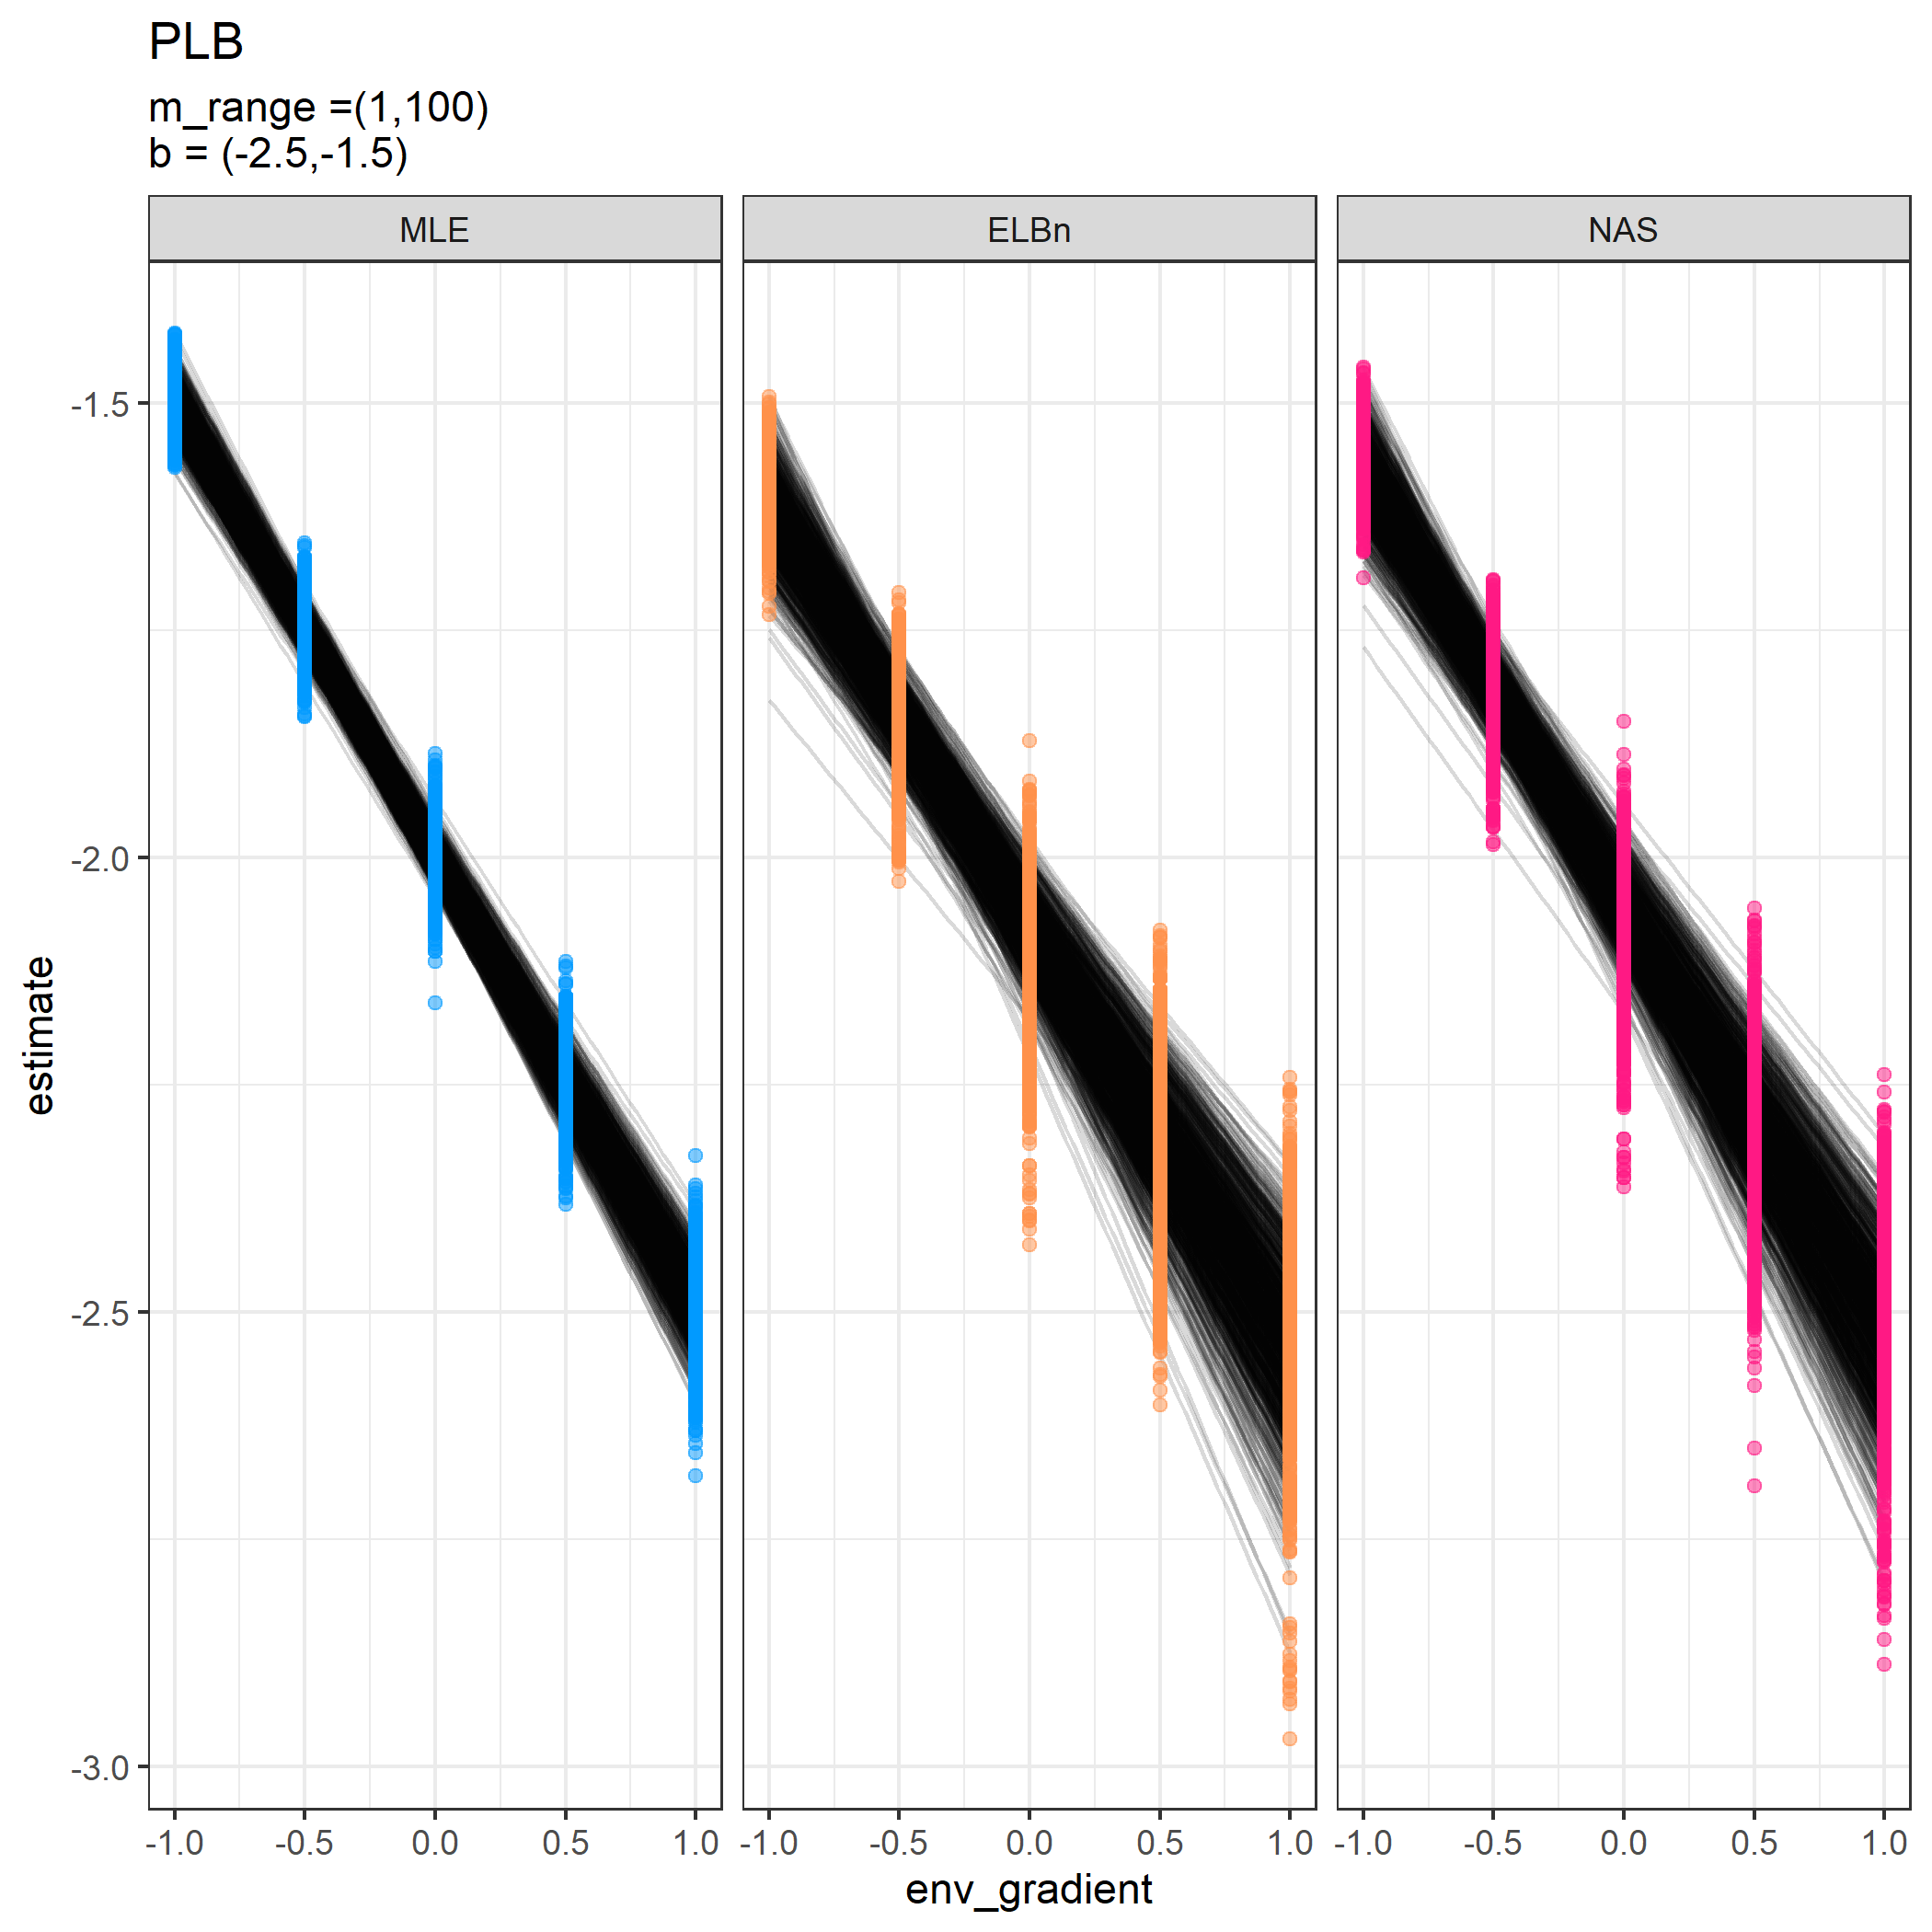
\includegraphics{figures/PLB_small_m_main.png}
\caption{Individual regressions for five sites across a hypothetical
gradient with a known relationship of 0.5. Range of body sizes is
reduced and is from 1, to 100.}
\end{figure}

\newpage

\begin{figure}
\centering
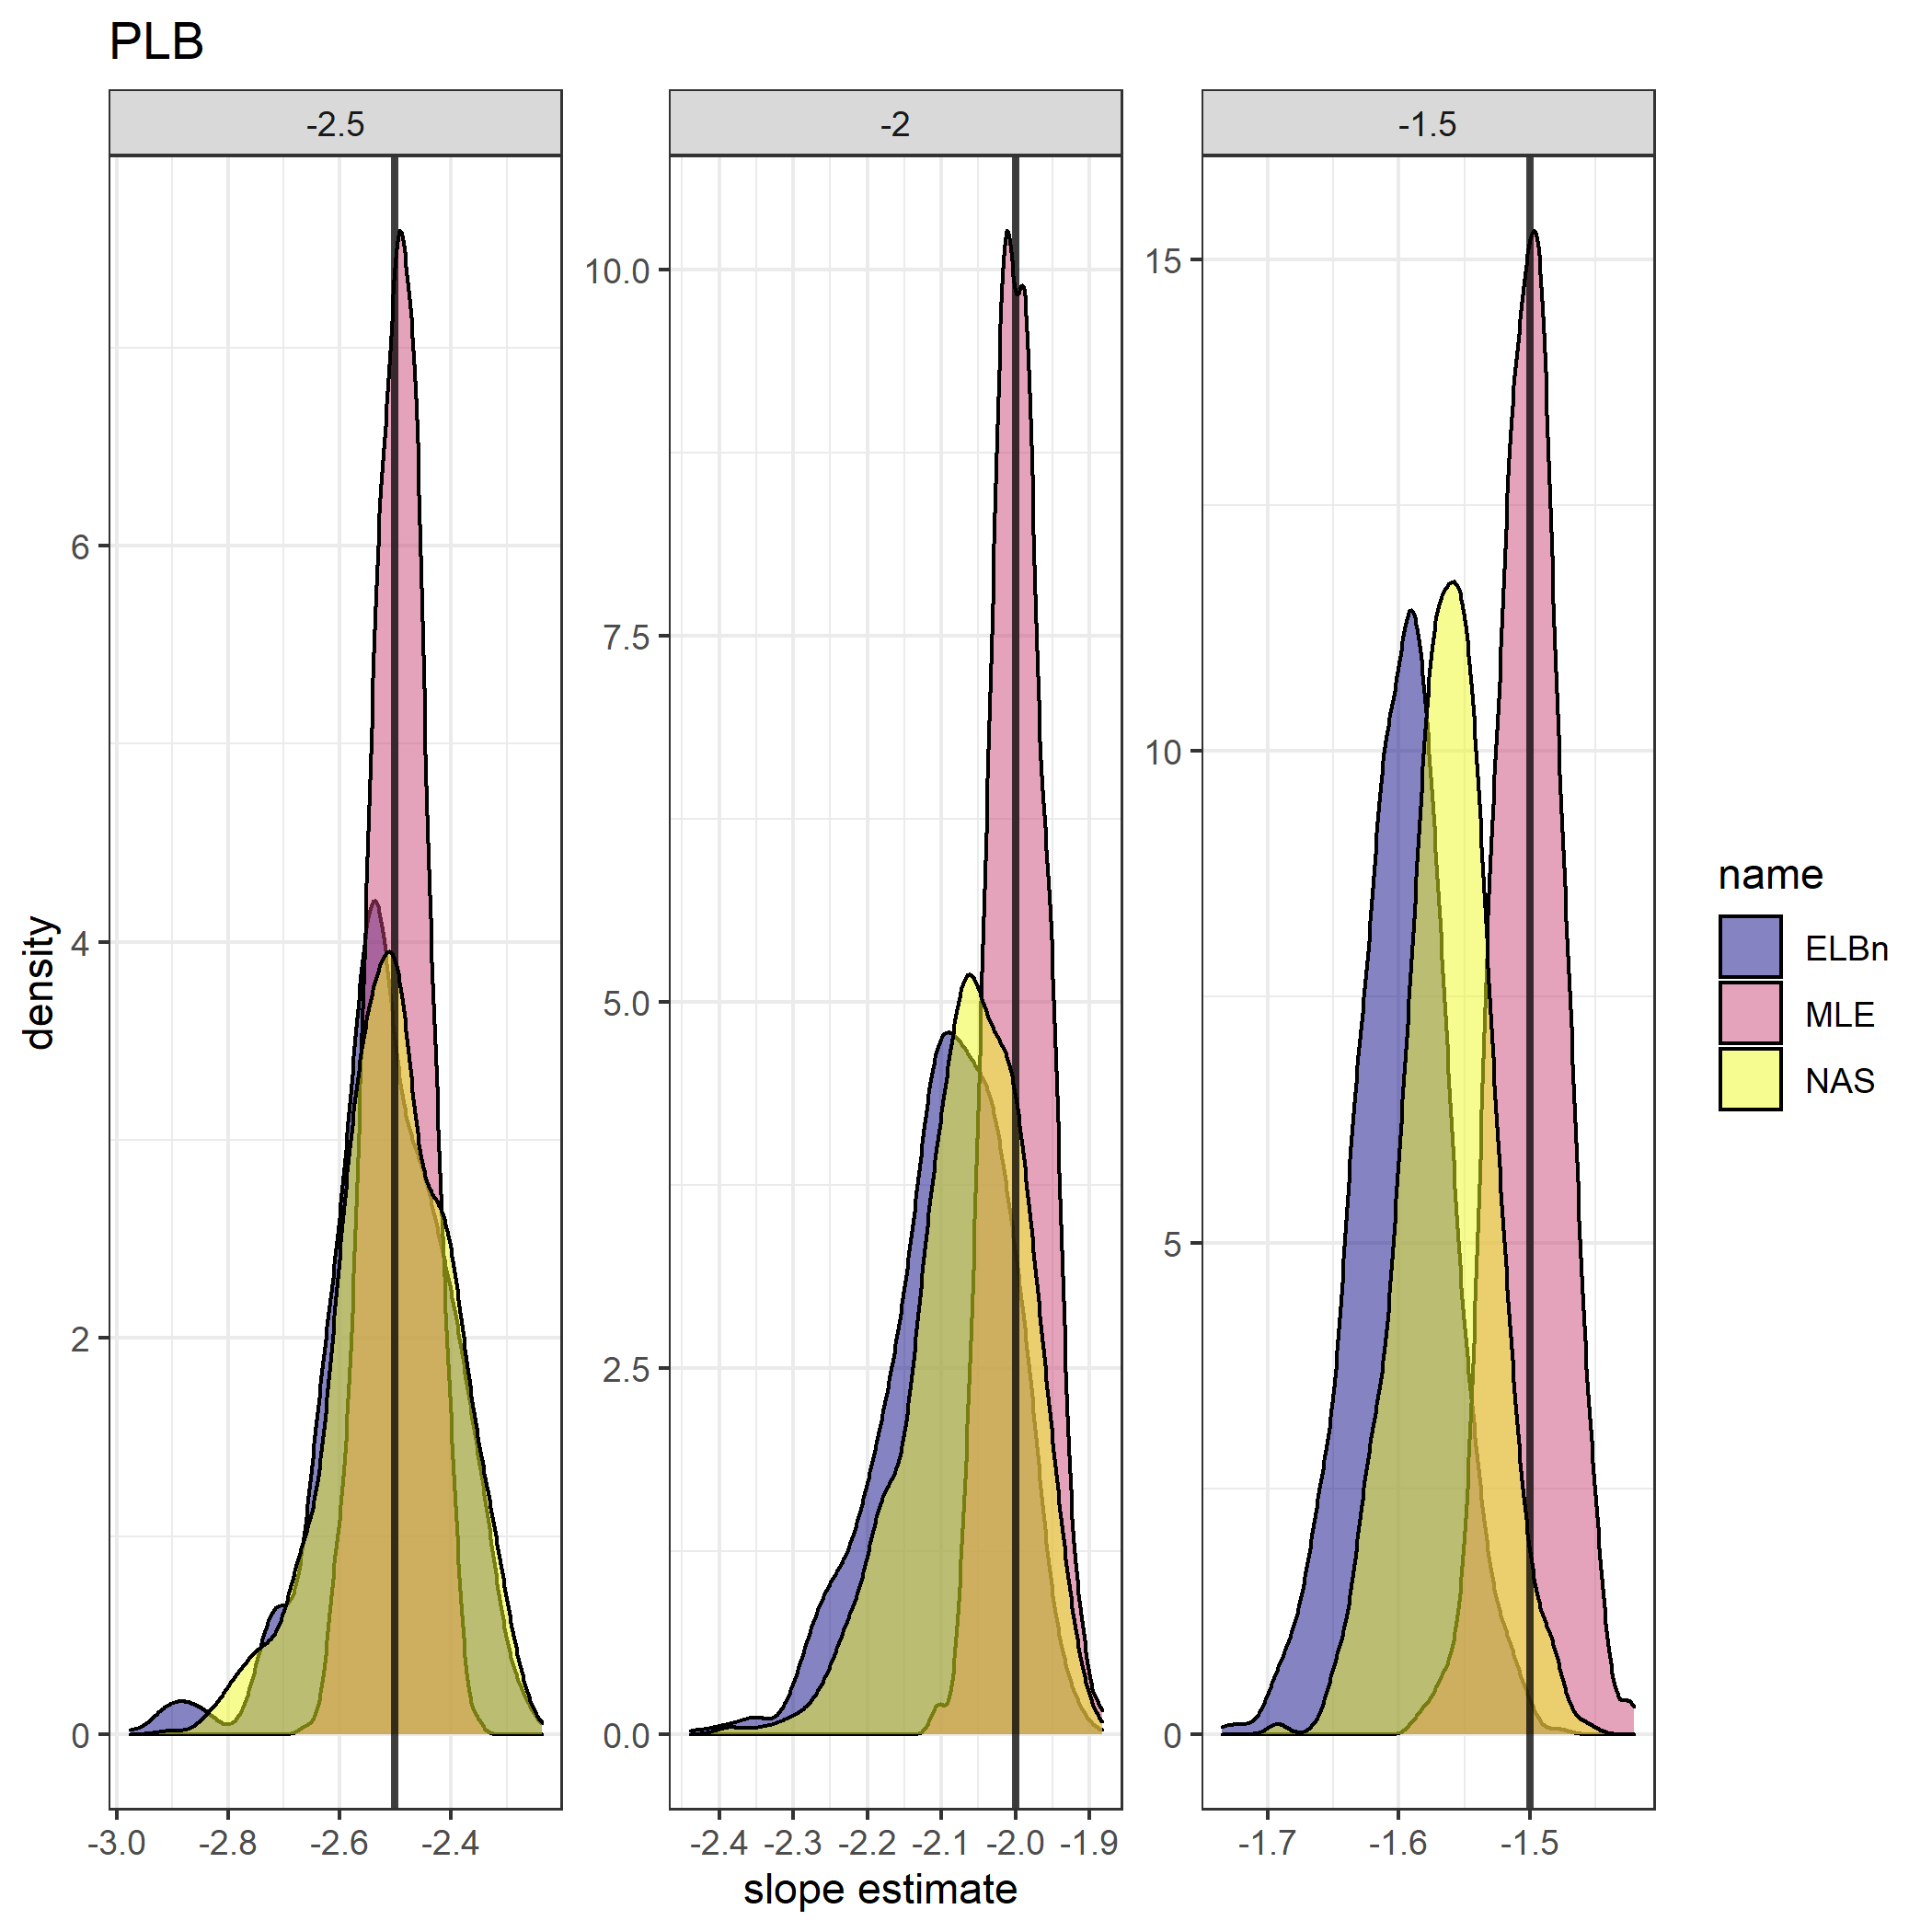
\includegraphics{figures/PLB_small_m_est_b_density.png}
\caption{Distribution of estimated \$\textbackslash lambda\$ coefficient
for five sites across a hypothetical gradient with known values(dashed
line). Range of body sizes is smaller than main anaysis and ranges from
1, to 100.}
\end{figure}

\begin{figure}
\centering
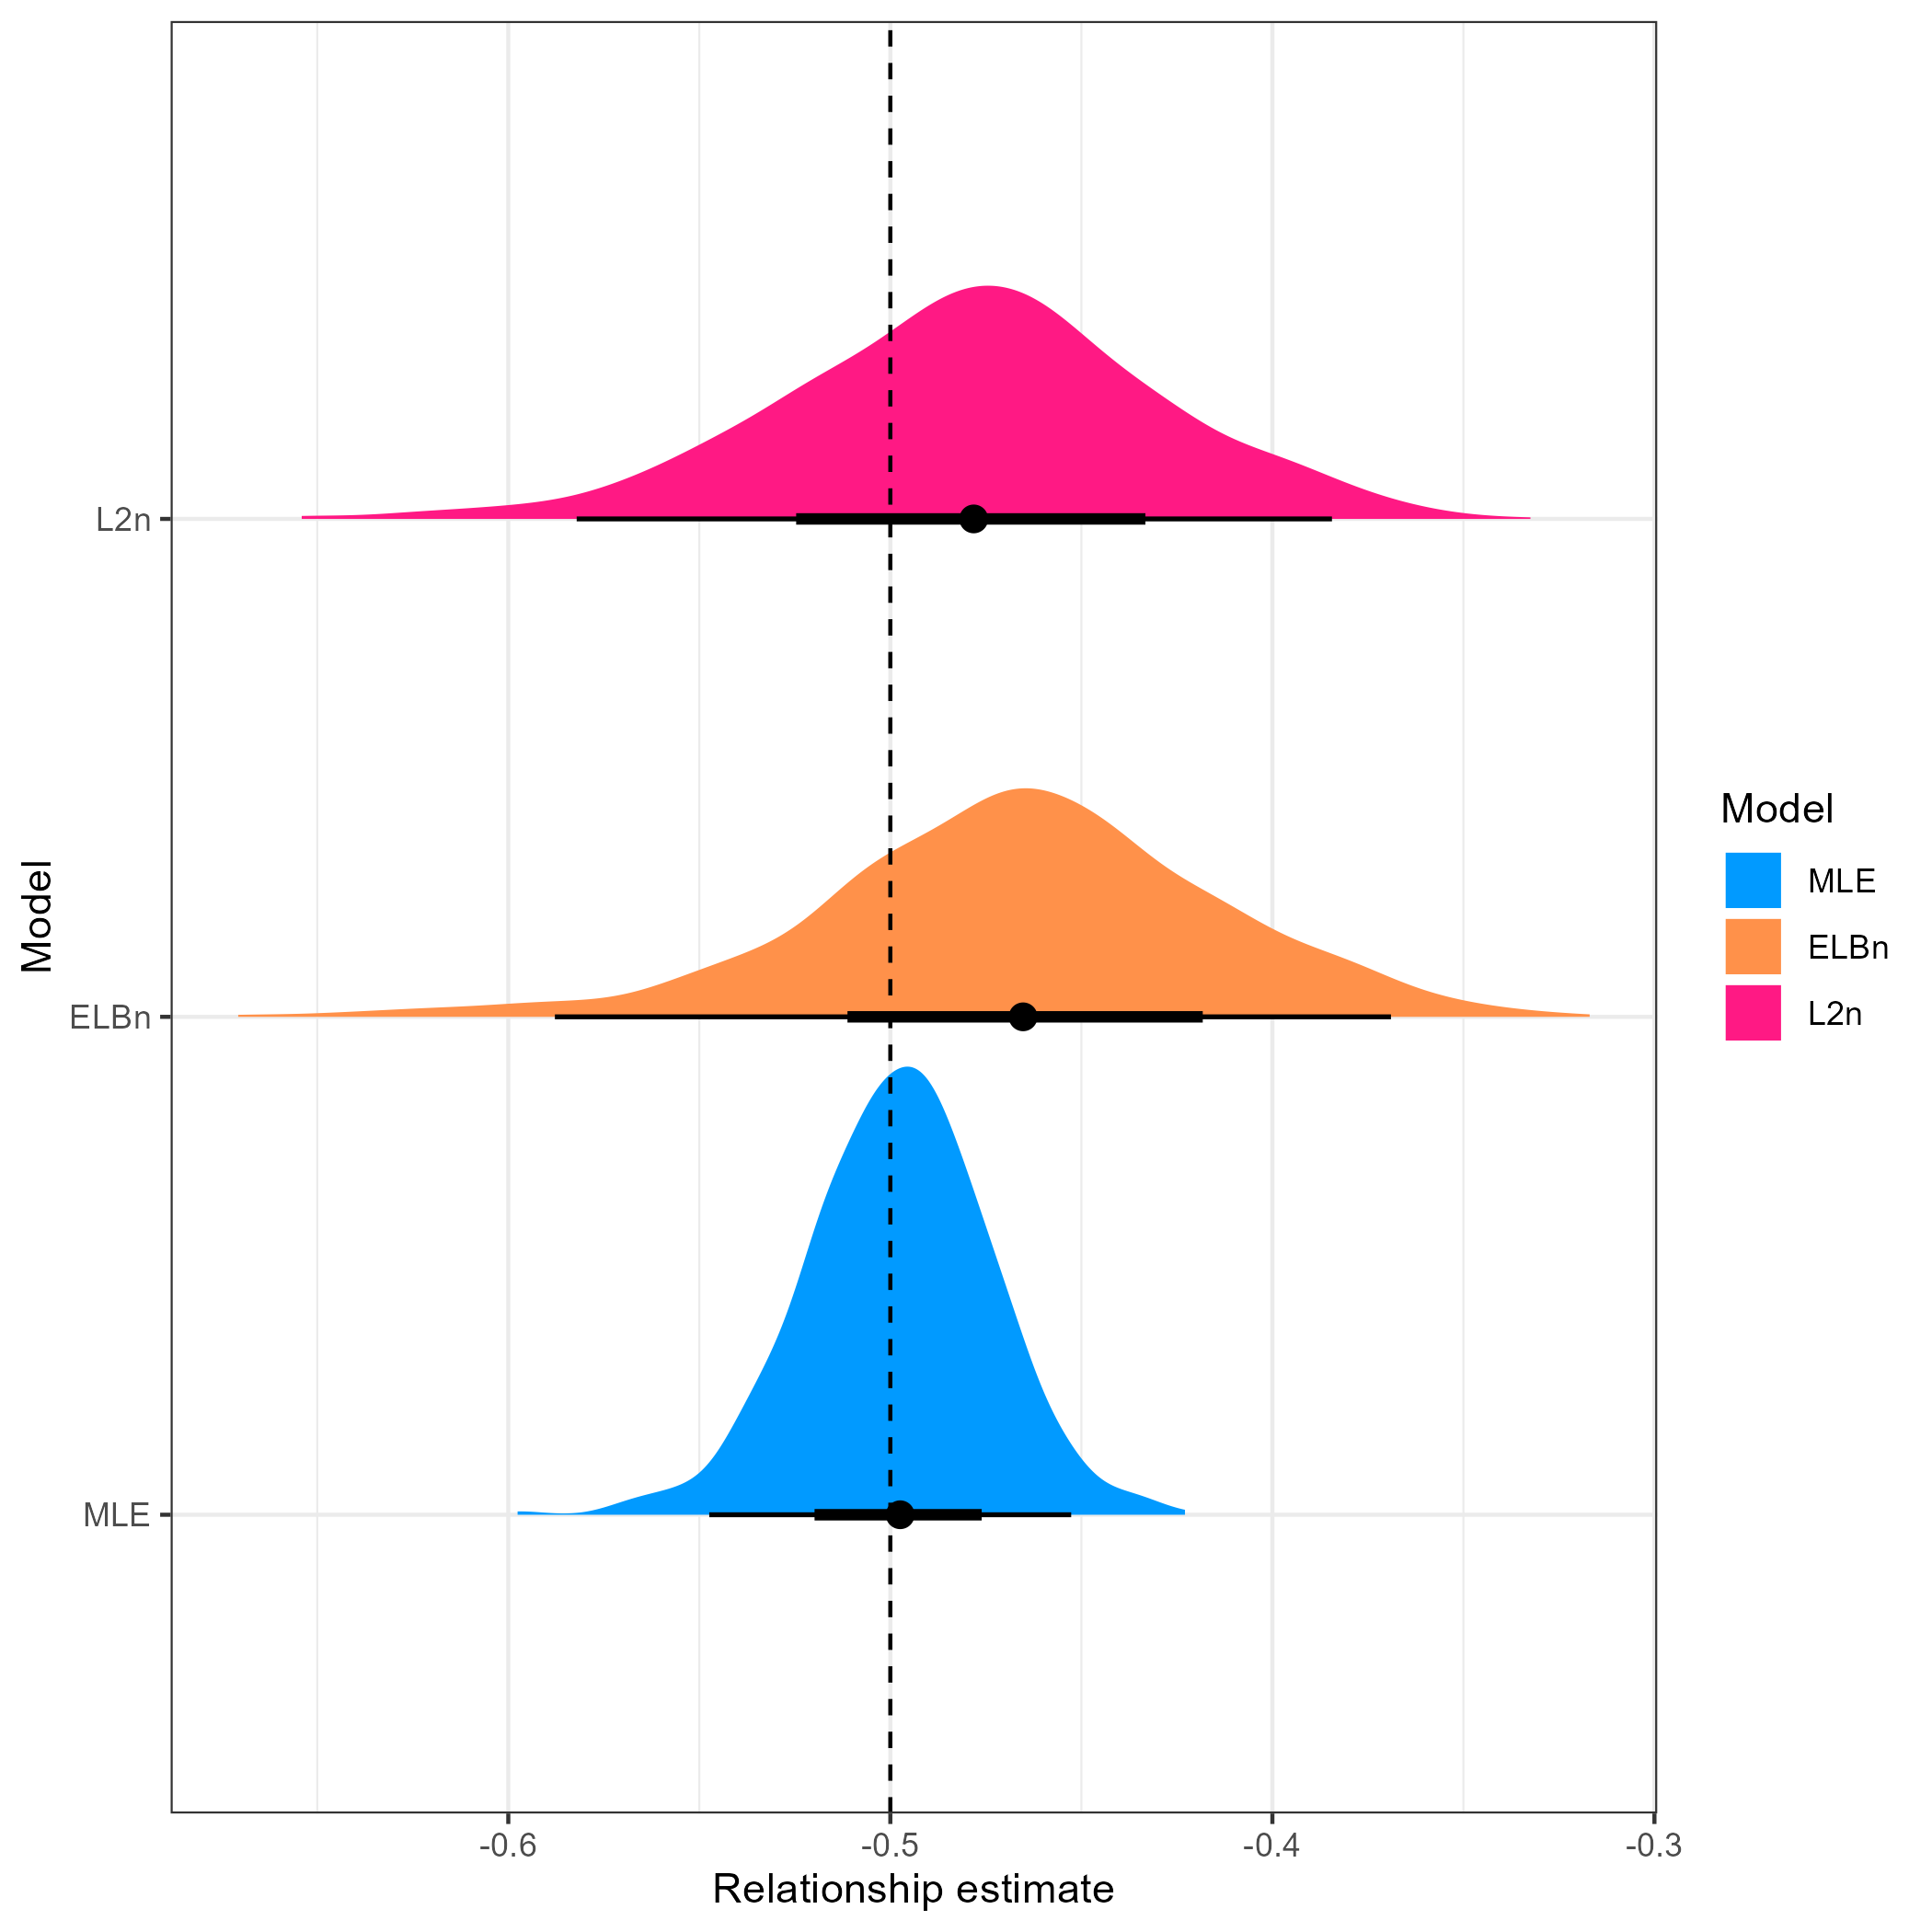
\includegraphics{figures/PLB_small_m_relationship_density.png}
\caption{Distribution of estimated relationship (\(\beta_1\))
coefficient's for five sites across a hypothetical gradient with known
value of 0.5. Range of body sizes is reduced and is from 1, to 100.}
\end{figure}

\newpage

\hypertarget{sample-size-n}{%
\subsection{\texorpdfstring{Sample size,
\(n\)}{Sample size, n}}\label{sample-size-n}}

The number of observations in our simulations may bias the results.
Therefore, we repeated the simulations described above, but varied the
sample size \(n\). We tested values of
\(n = 200, 500, 1000, 5000, 10 000\). Results of this analysis are
presented in the Supplemental Information.

\begin{figure}
\centering
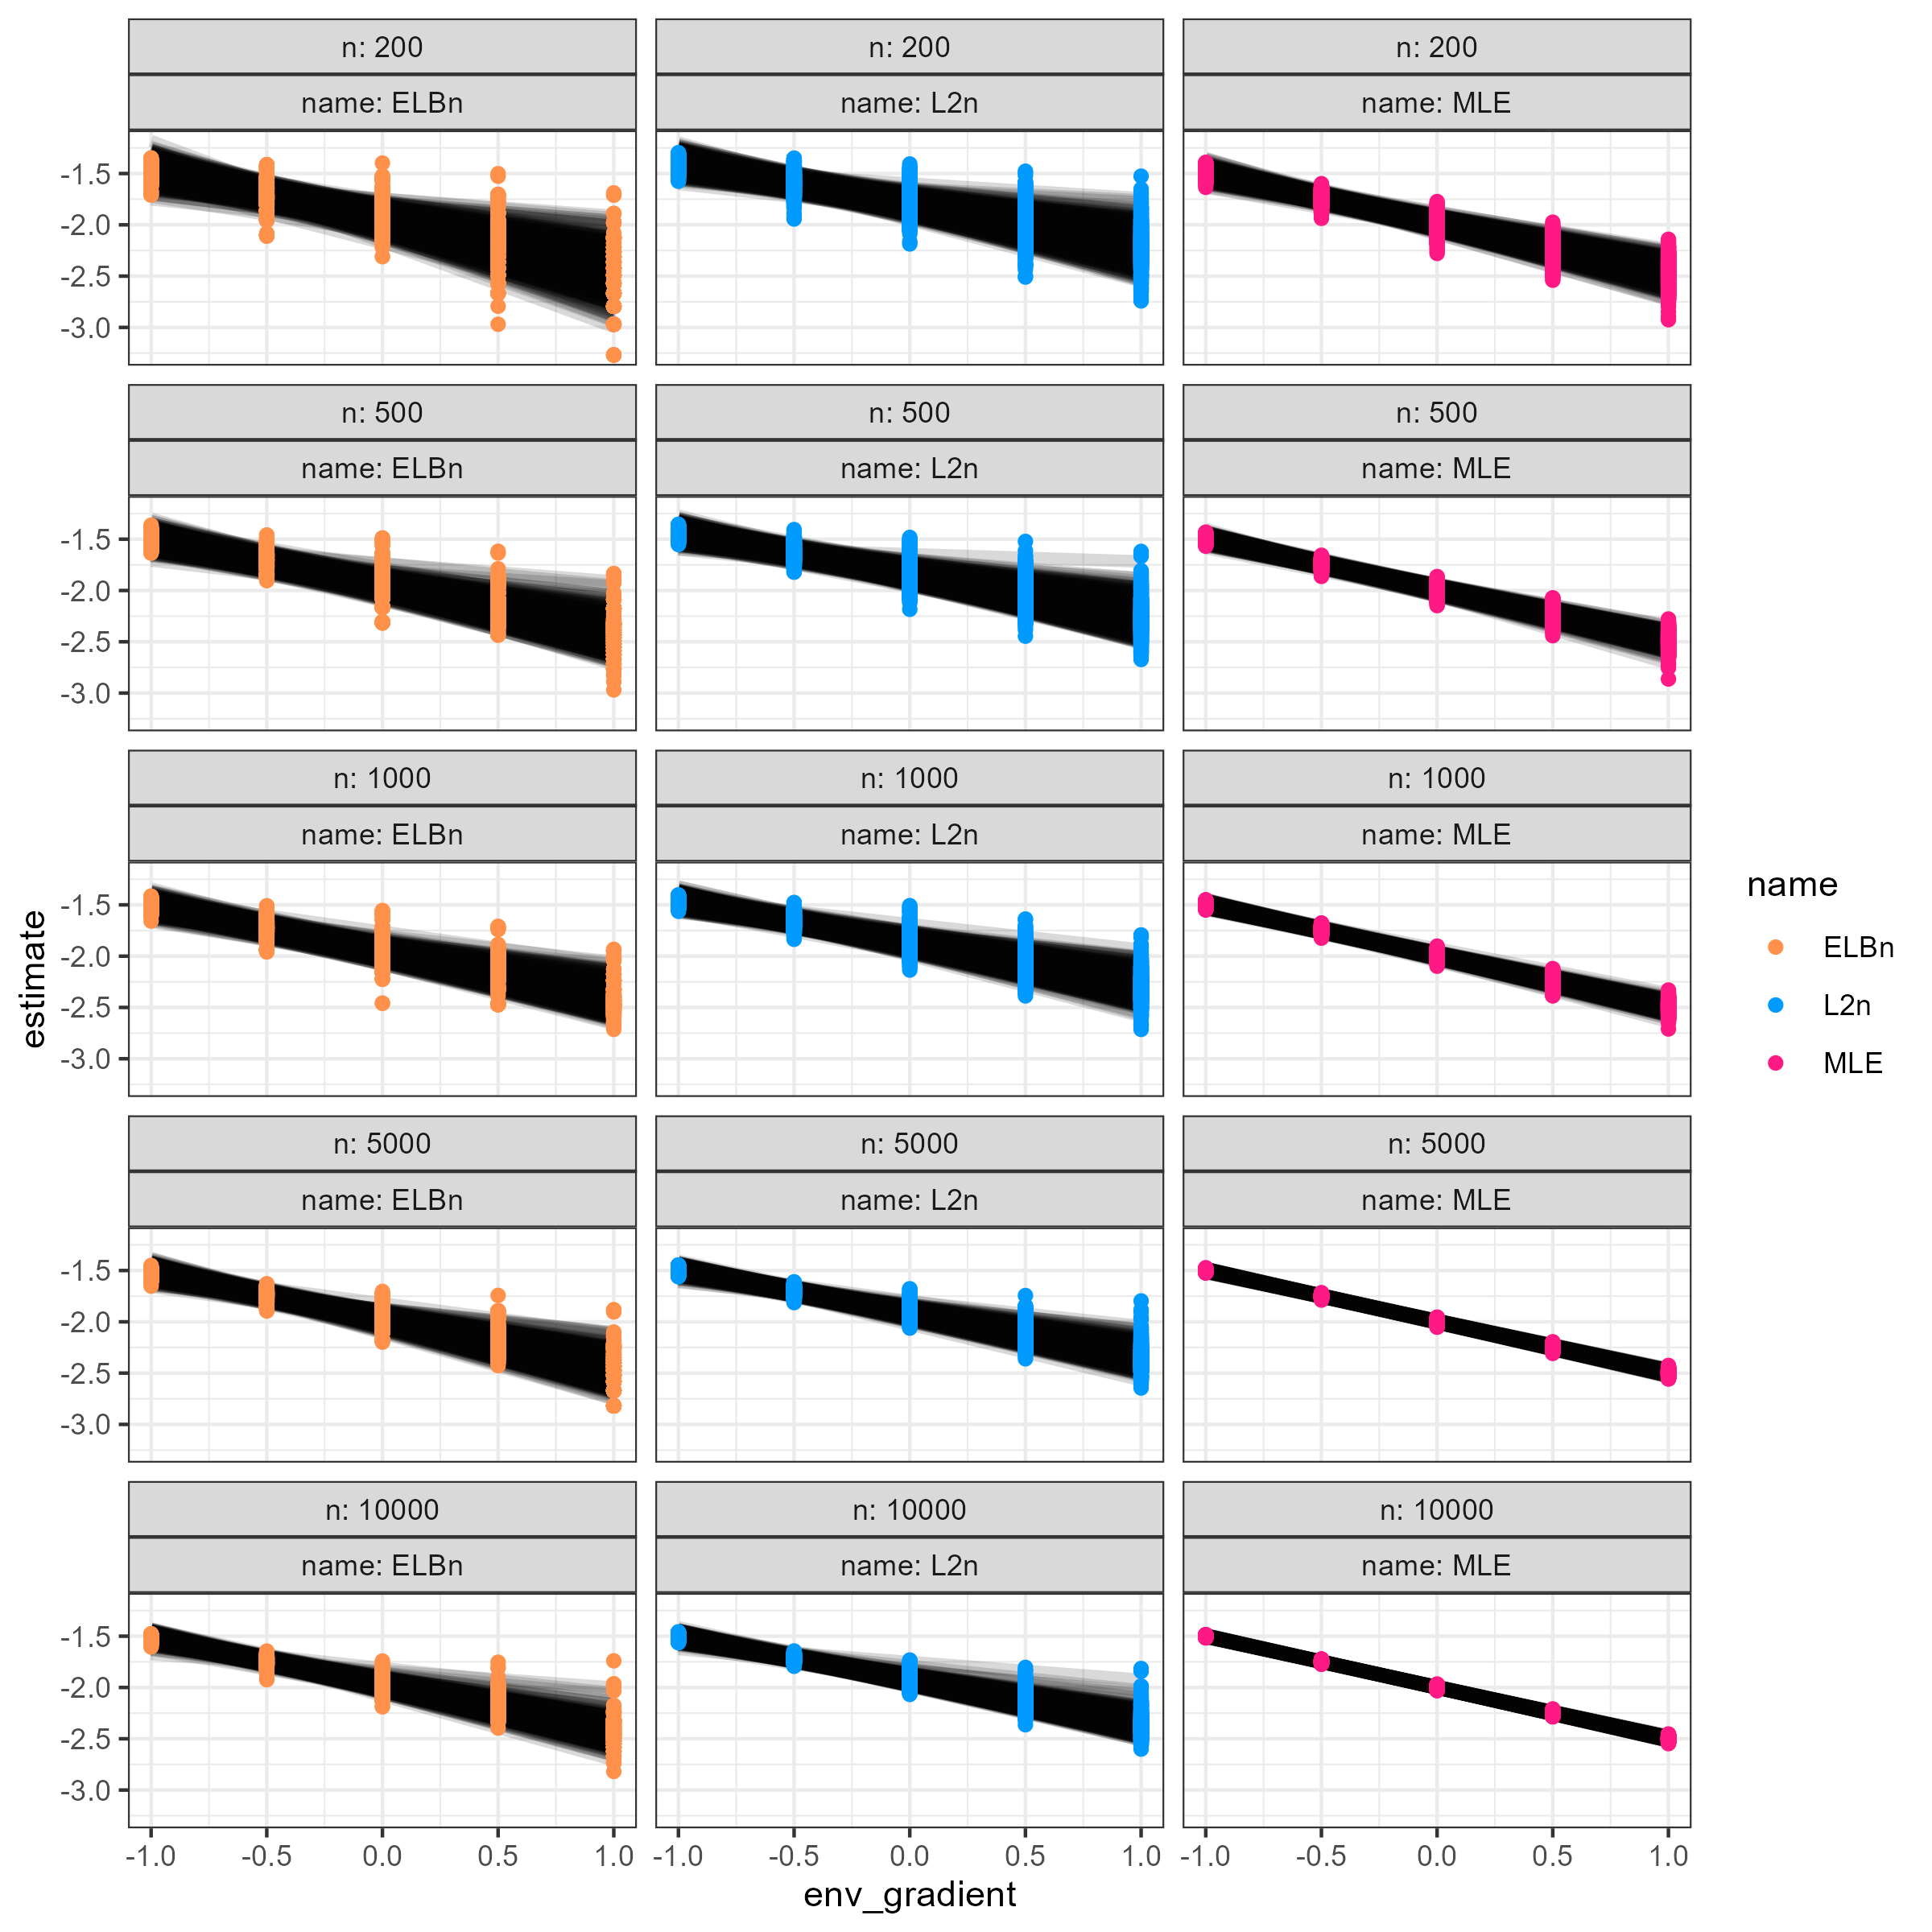
\includegraphics{figures/n_vary_main.png}
\caption{Individual regression estimates across the hypothetical
gradient based on sample size (rows) and methodology used (columns).
(match this figure to ``new'' style if we like that better)}
\end{figure}

\begin{figure}
\centering
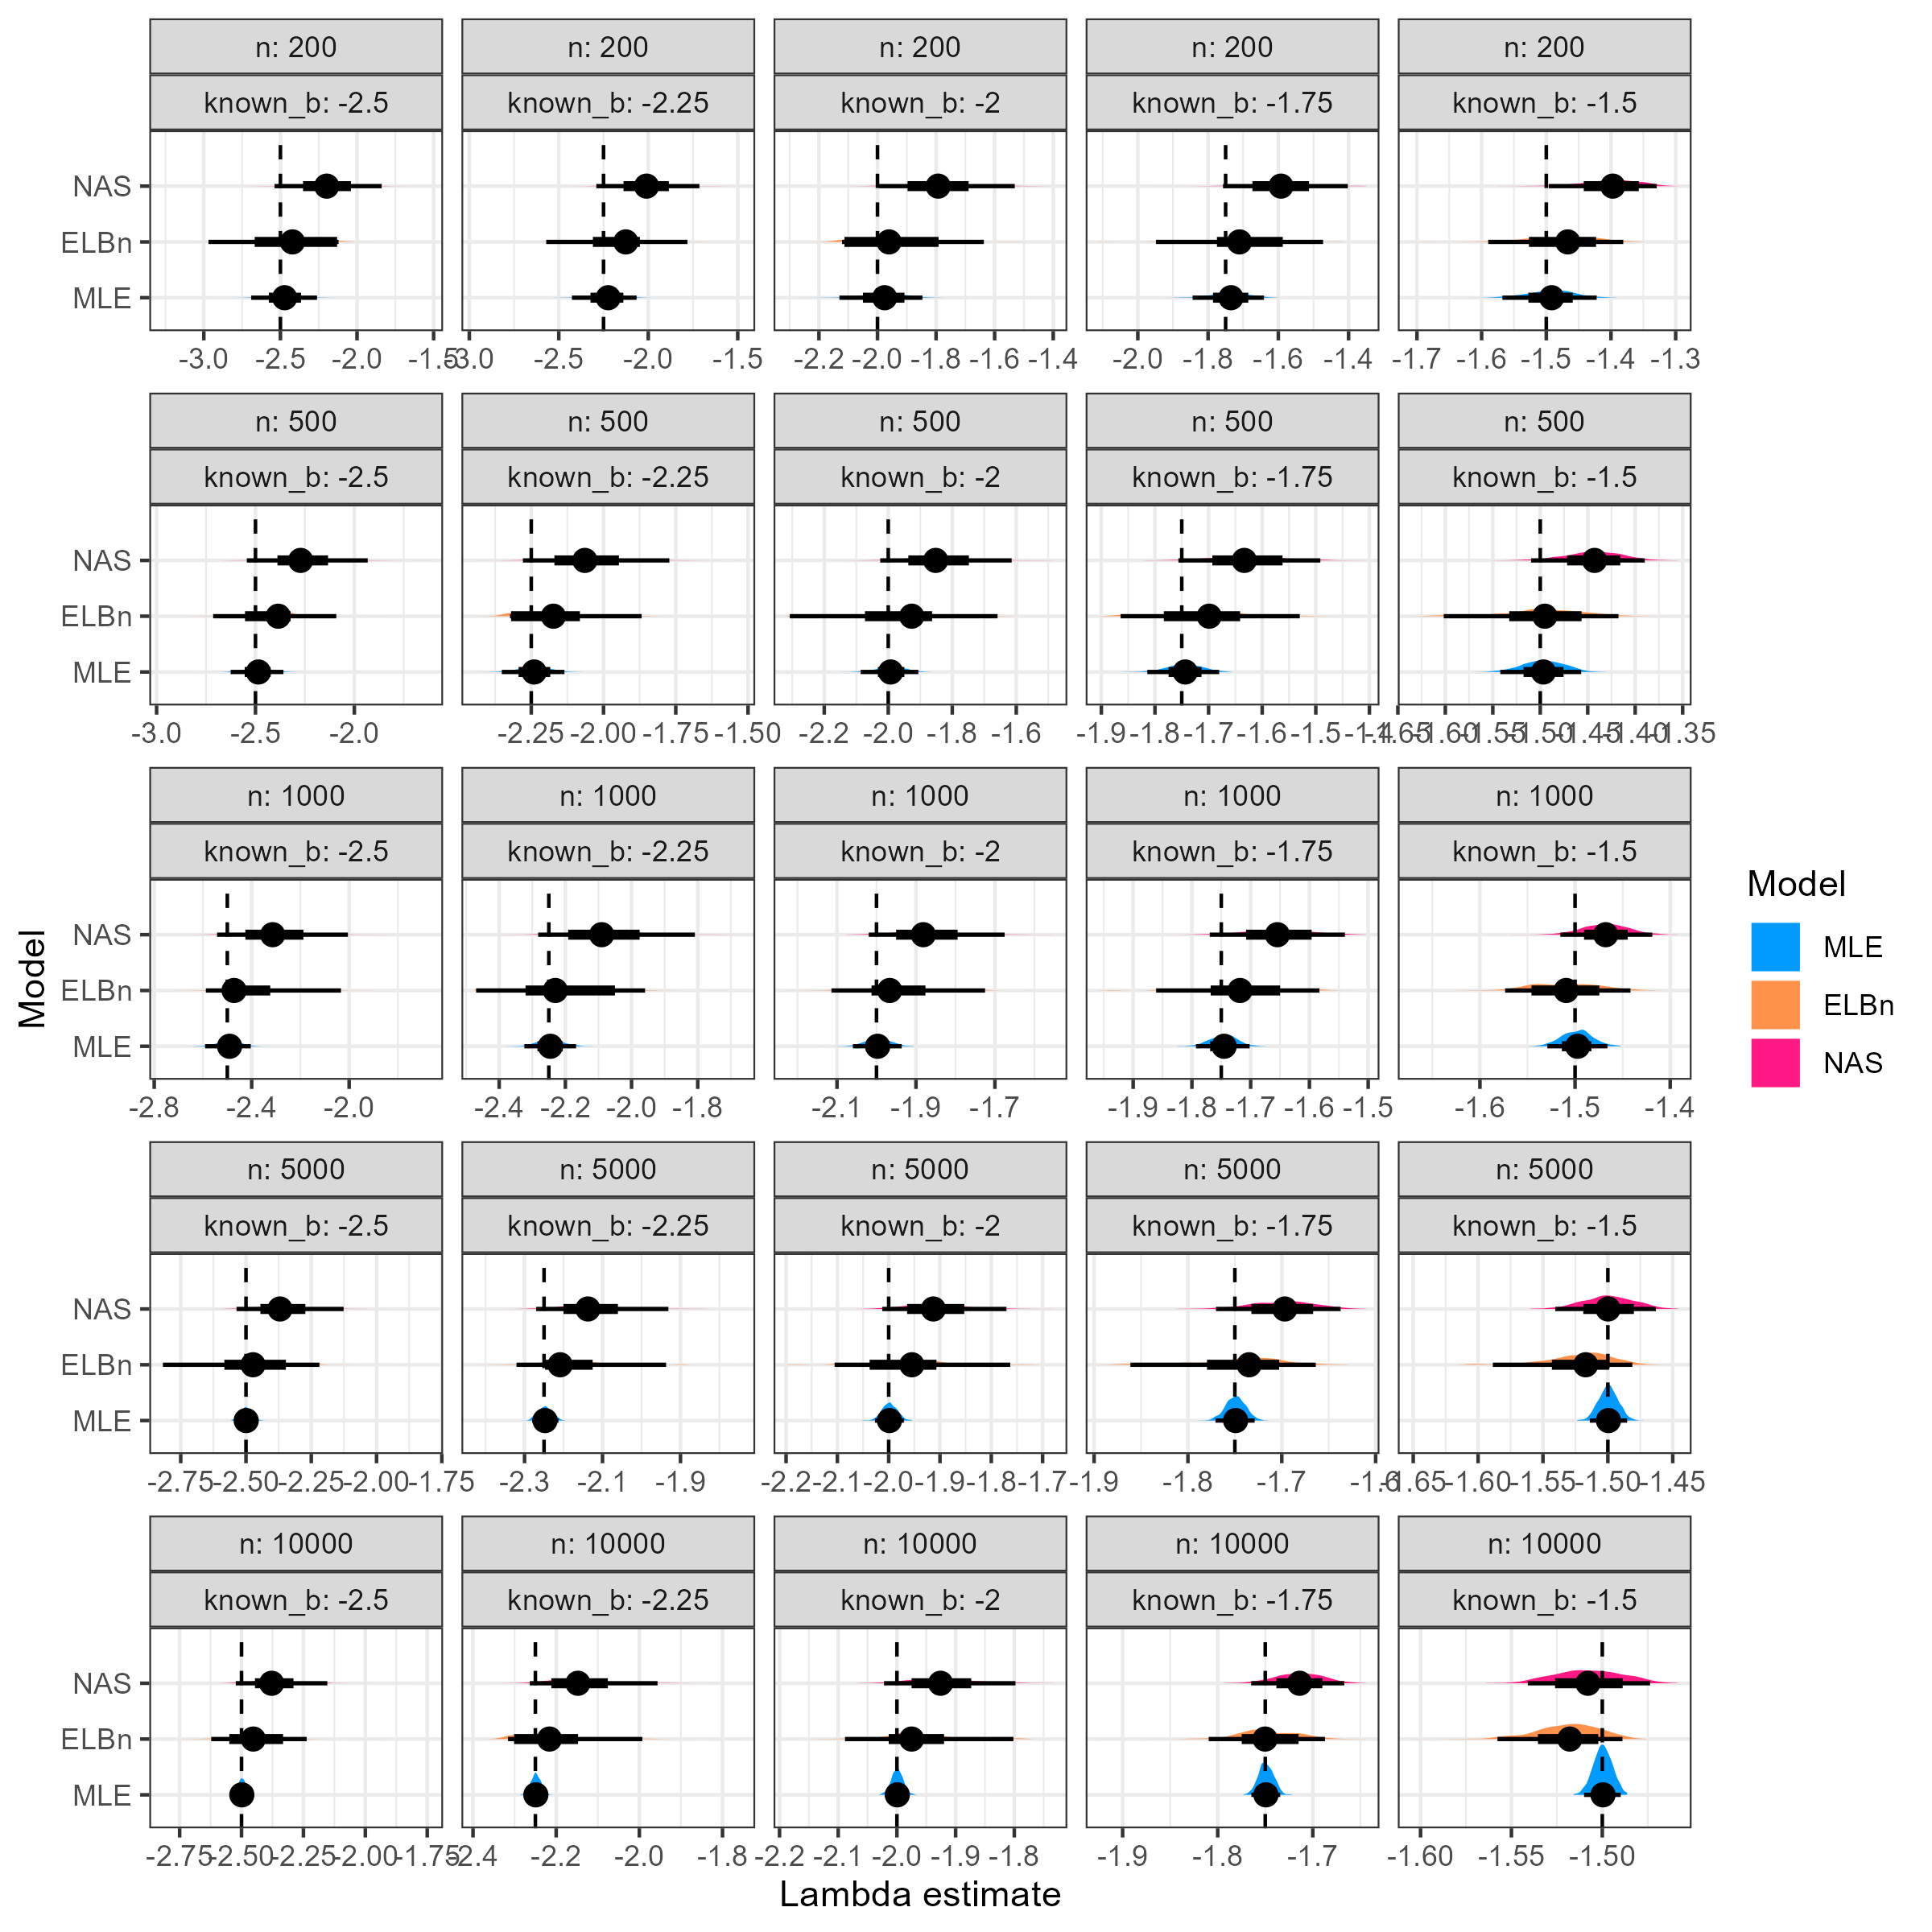
\includegraphics{figures/n_vary_est_b.png}
\caption{Distribution of size spectra parameter estimates. Vertical line
is the known parameter (dashed line) wich describes the bounded power
law distribution from which the body size estimates were sampled. As n
increases (top to bottom) and \(\lambda\) increases (left to right), the
accuracy of the estimate improves across all methods.}
\end{figure}

\newpage

\begin{figure}
\centering
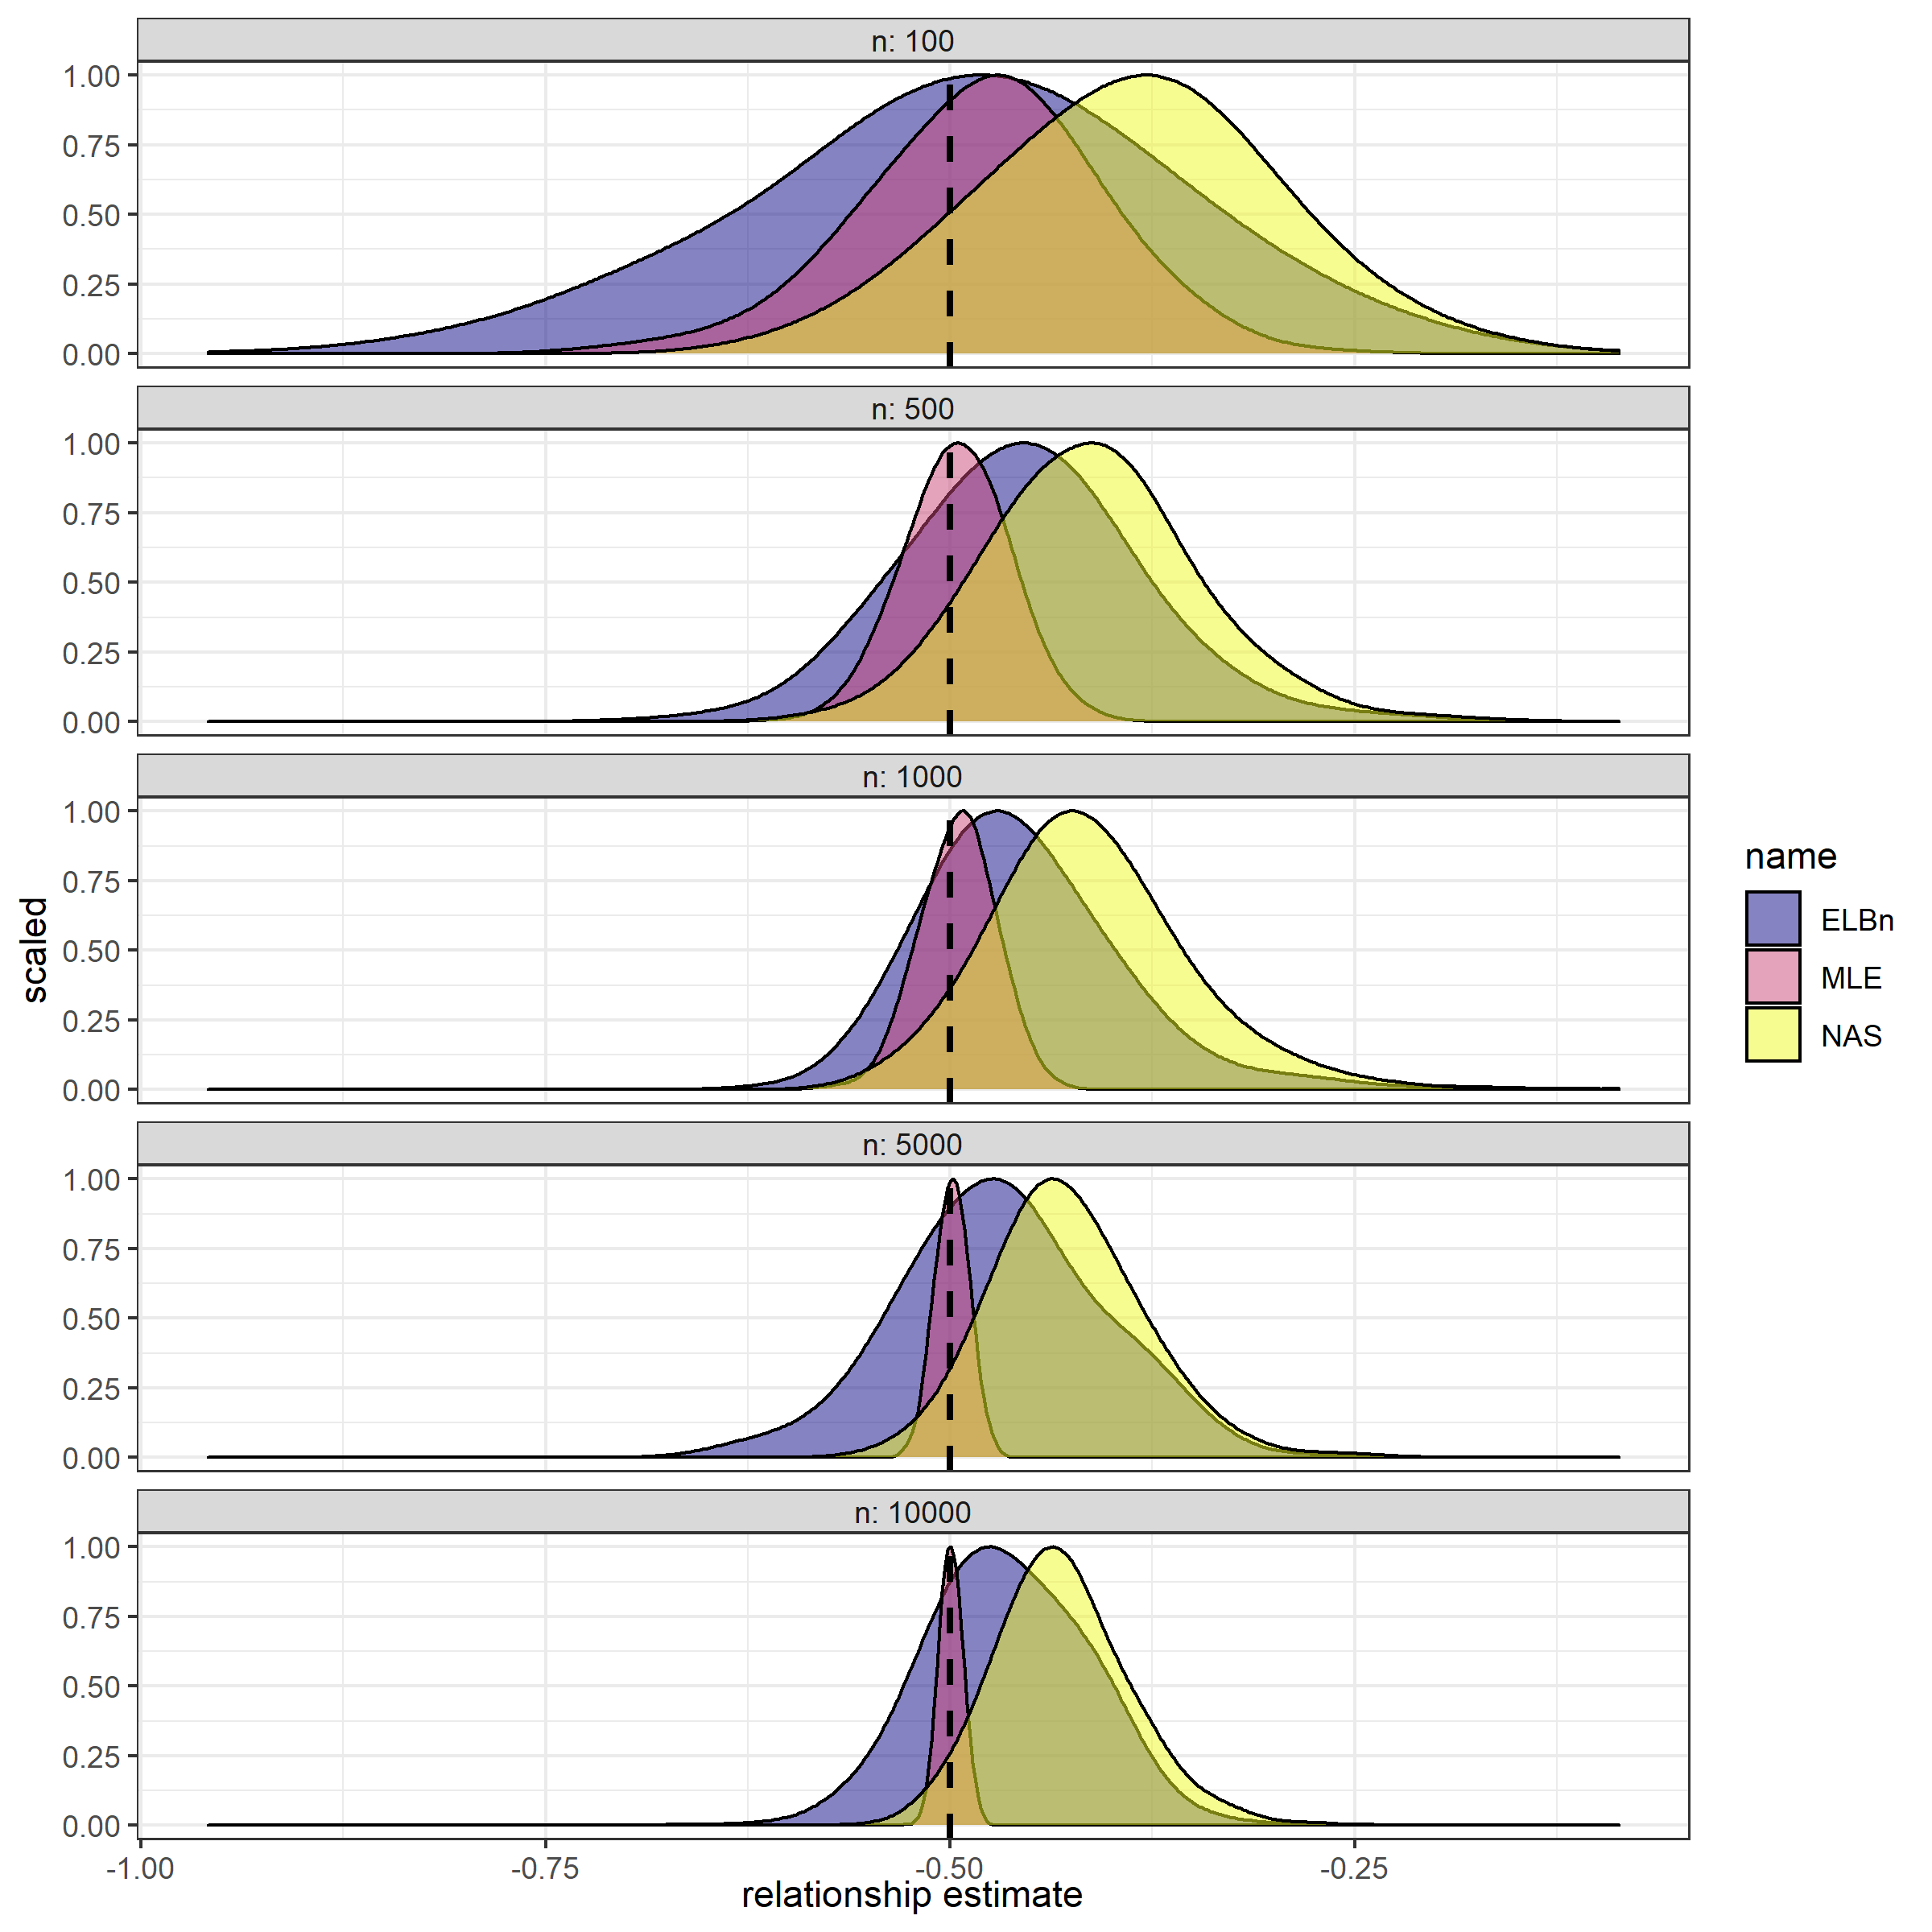
\includegraphics{figures/n_vary_relationship_density.png}
\caption{Distribtuion of the relationship coefficients with varying
sample size}
\end{figure}

\hypertarget{comparison-with-other-published-estimates}{%
\section{Comparison with other published
estimates}\label{comparison-with-other-published-estimates}}

SI Table. This table shows published estimates of the variation in size
spectra slopes (or exponents) in empirical studies. It is unclear how to
directly compare estimates of the slope with different methods. However,
the published estimates here range from \textasciitilde0.1 to 0.2 across
the gradients studied. For comparison, the 2.5-95\% quantiles around the
relationship estimate for the MLE method were \textasciitilde0.1,
whereas for the ELBn and NAS method they were \textasciitilde0.25 and
\textasciitilde0.2, respectively. b\_diff is the change in estimate
(b-low - b-min). System refers to stream communities or mesocosm
experiments. Method: MLE = maximum likelihod estimate, ELB = equal
logarthmic binning, the number before indicates the number of bins used.
The normalization process shifts the estimates by an absolute value of
1.0. Hence, direct comparison the relative change in normalized and
non-normalized studies should not introduce any bias. The O'Gorman et
al.~2017 study used average species size and abundance (Local Size
Density Relationship, \emph{sensu} White et al.~2007) as opposed to
individual size distribution. These methods are related, but it is
unclear how to directly compare estimates from each method.

Supplementary table comparing with other published results will be
submitted as a separate file for formatting.

\end{document}
